%Hauptdokument der Erstsemesterzeitschrift "Erste" der Fachgruppe Informatik
% TO DO:
% - Anpassen der Anrede: entweder du oder ihr
% - Rechtschreibkorrektur
% - Aktualisierung von Beiträgen
% - Recherche nach neuen Bildern
% - Rechteklärung mit den Profs wegen Fotos
% - 
\documentclass[]{papertex}
	\usepackage[utf8]{inputenc}
	\usepackage{graphicx}
	\usepackage{amssymb}
	\usepackage[T1]{fontenc}
	\usepackage{multicol}
	\usepackage[babel,german=quotes]{csquotes}

	\renewcommand{\familydefault}{\sfdefault}

	\clubpenalty = 10000
	\widowpenalty = 10000 
	\displaywidowpenalty = 10000

	% Trennregeln
	\hyphenation{
		AStA
		Mit-be-wohnerIn-nen
		Pro-fessorInnen
		erwischt
		viiieel
		y-Nummer
		Uniaccount
	}

\begin{document}
	\thispagestyle{empty}
	\clearpage
	\setcounter{page}{1}
	\tableofcontents
	\newpage
	% !TEX root = ../1-te.tex

\section{Vorwort}
\label{vorwort}
	\begin{multicols}{2}
	\subsection*{Willkommen in der Informatik!}	

	Das neue Semester an der TU Braunschweig beginnt und du bist dabei. Die Fachgruppe Informatik (s. Seite \pageref{fachgruppe}) begrüßt dich ganz herzlich an der Uni und möchte dir mit der \enquote{1-ten} den Start vereinfachen. Diese Erstsemesterzeitung der Informatiker soll dir dabei helfen, Antworten auf viele Fragen, die sich zu Beginn des Studiums stellen, zu beantworten.

	\subsubsection*{Aufbau dieses Heftes}
		Der Fokus der ersten Seiten liegt auf den vielen Fragen zum Studienbeginn, deinem Studiengang und der Infrastruktur der Uni. Wir erklären, wie Studienplanung funktioniert und was für Bachelor und Master wichtig ist.
Der Fachgruppenrat Informatik stellt sich vor und beantwortet die Fragen, wer er ist und was er macht.


	\columnbreak

	\begin{center}
		
\includegraphics[width=.7\columnwidth]{bilder/fg-logo/fg-logo.pdf}
	\end{center}

	\subsubsection*{Der Blog}
		Der Fachgruppenrat Informatik betreibt den Blog FGInfo (\fginfoUrl). Dort werden unsere Termine und Veranstaltungen, z.B. Spieleabende, angekündigt und über die hochschulpolitische Arbeit berichtet.
Zusätzlich pflegt die Fachgruppe ein Wiki mit vielen Infos, Tipps und Wissenswertes rund um die Informatik-Studiengänge.
Dieses Heft, die 1-te, gibt es dort auch noch einmal zu finden. Mitunter
ergeben sich noch nach dem Druck Änderungen, gerade bei Terminen, also schau auf jeden Fall dort rein!

	\vspace*{0.5cm}

	Viel Spaß und Erfolg im  Studium wünscht  die\\
	\hspace*{2cm}Fachgruppe Informatik

	\end{multicols}
 %Import ohne Seitenumbruch
	\newpage
	\section{Die ersten Tage}
		\subsection{Termine}
\label{termine}
Gerade in der Anfangszeit des Studiums gibt es eine Menge zu tun. Damit ihr
nicht das Wichtigste verpasst, haben wir die ersten Termine kompakt für
euch zusammengefasst. Die meisten davon bieten die Gelegenheit Fragen zu
stellen und nebenbei gleich ein paar nette Kommilitonen kennen zu lernen.

Falls ihr es euch nicht schon gedacht habt: Die Spalten B und M geben an,
ob der Termin für Bachelor- oder Masterstudenten gedacht ist. Falls jemand
von euch den eigentlichen Termin verpasst, kann er meist ersatzweise auch
zum anderen erscheinen. Es besteht die Chance, dass sich einige Orte
und Zeiten
nach Drucklegung noch Ändern.  Bei den mit ,,*'' markierten Zeiten und
Orten ist das besonders wahrscheinlich. Schaut deshalb bitte vorher
nochmal im Blog \url{http://fginfo.cs.tu-bs.de/} nach, ob die Angaben
noch aktuell sind. Dort könnt ihr übrigens auch den Kalender digital abonnieren.
\end{multicols}
\begin{tabular}{|l|l|p{6.7cm}|c|c|c|}
\hline \textbf{Datum} 		& \textbf{Uhrzeit} 	& \textbf{Veranstaltung}						& \textbf{Ort} 	& \textbf{B}	& \textbf{M} 	\\
\hline 26.09. – 30.09.		& 1. Tag: 10:00	 	& Vorkurs Informatik							& PK 2.1		& B				& 				\\
	   17.10. – 21.10.		& 					& 												& 				& 				&    			\\
\hline Mo, 24.10. 			& 09:00 – 10:00		& Begrüßung	durch den Präsidenten				& Stadion		& B				& M				\\ 
\hline 						& 10:00 – 12:00	 	& Infobörse										& Altgebäude	& B				& M				\\
\hline   					& 10:00 – 11:00	 	& Begrüßung (M) \newline durch den Studiendekan	& IZ 160		& 				& M				\\
\hline 						& 14:00 – 15:00	 	& Begrüßung (B) \newline durch den Studiendekan	& PK 11.3		& B				& 				\\
\hline 						& 15:00 – 16:30		& Erste Vorlesung ,,Programmieren 1''			& SN 19.1		& B 			&				\\
\hline Di, 25.10.			& 10:00 – 11:45 	& Erstsemester-Frühstück 						& IZ Plaza 		& B 			& M 			\\ 
\hline 						& 12:00 – 13:30 * 	& FG-Einführung und \newline Stundenplan-Bauen 	& ??? * 		& B 			&  				\\%& ??? * & B &\\
\hline 						& 12:00 – 13:30 * 	& FG-Einführung und \newline Stundenplan-Bauen 	& IZ 160 * 		& 				& M				\\
\hline 						& 13:30 – 15:00 	& Rundgang mit den  Tutorengruppen 				& IZ 160 		& B 			& M				\\
\hline Mi, 26.10.			& 10:00 – 17:00		& Studium Generale								& Altgebäude	& B				& M 			\\
\hline Do, 03.11. 			& 19:00 			& Kneipentour der Fachgruppe 					& IZ 150 		& B 			& M				\\
\hline Mi, 09.11.	 		& 19:00 			& Spieleabend der Fachgruppe 					& vor  150 		& B 			& M				\\
\hline
\end{tabular} 
\begin{multicols}{2}

%Zum besseren Verständnis der Spalte \textit{Ort} schau in den Abschnitt \textit{Campuskarte} auf Seite \pageref{campuskarte}.

%TODO folgendes muss dann aber auch wirklich umgesetzt werden:
Ihr findet die Termine auch online unter \url{http://tinyurl.com/3ltuzbb}.
Falls ihr einen Dienst, ein Handy oder eine Software nutzt, die das iCalender-Format unterstützt
könnt ihr die Termine auch von dort aus einbinden und habt sie somit im Blick. 
Dazu gehören z.\,B. iPhone, Android, Google Calendar, Outlook\,\dots. Eine Liste 
von ca. 60 Programmen findet ihr unter 
\url{http://tinyurl.com/yns84t}


% TODO es wäre schön, hier zu jedem Termin noch ein oder zwei Sätze zu schreiben, damit man sich darunter etwas vorstellen kann, ähnlich wie bei der TODO-Liste, wo ja auch diverse Textabschnitte folgen.

%In der \textit{Ort}-Spalte stehen meist Raumnummern. F"ur alle R"aume die nicht
%im IZ (steht f"ur Informatikzentrum) liegen, schaut am besten auf den
%Campusplan im Einband. Bei den R"aumen im IZ ist die erste Zahl das Stockwerk, f"ur
%den Rest m"usst ihr dann auf den Plan im Stockwerk schauen (Kleine Falle:
%zwischen EG und 1. OG liegt das Galeriegescho"s - Raum IZ 150 liegt also
%effektiv in der zweiten Etage).
% - Gl"uhweinabend im Informatikzentrum (IZ)

% Dieser Trick hilft uns, eine neue Seite zu erzwingen
% (auf diese passt eh nix sinnvolles mehr) und dennoch die 
% Spaltenlängen auszubalancieren.
\end{multicols}
%    \begin{center}
%          \includegraphics[width=\linewidth]
%	  {bilder/comics/phd092706s.png}    \end{center}
\newpage
\begin{multicols}{2}


%%% Local Variables: 
%%% mode: latex
%%% TeX-master: "../../1-te"
%%% End: 

		% !TEX root = ../../1-te.tex

\subsection{Checkliste}
\label{checkliste}
	Hier wird zusammengefasst, was du in den ersten Tagen des Studiums unbedingt erledigen solltest. Wenn du die ToDos auf der Checkliste nach Erledigung abhakst, verlierst du nicht den Überblick und vergisst nichts.
	
\vspace*{0.5cm}
% !TEX root = ../../1-te.tex

\begin{tabular}{|p{3mm}|l|l|c|c|}
\hline \checkmark 
       & \textbf{Todo}             & \textbf{Zu erledigen bis}                                  & \textbf{Seite}               & \textbf{Muss?} \\ 
\hline & BAföG beantragen          & Spätestens Ende \iftoggle{winter}{Oktober}{April}          & \pageref{todobafoeg}         & optional \\ 
\hline & Wohnsitz Ummelden         & 1 Woche nach Umzug                                         & \pageref{todoummelden}       & ja \\ 
\hline & Mailinglisten             & So früh wie möglich                                        & \pageref{mailinglisten}      & ja \\ 
\hline & Studiengrobplanung        & Vor dem Stundenplanbauen                                   & \pageref{grob}               & ja \\ 
\hline & Auflagen klären           & So früh wie möglich, final: Ende 2. Semester               & \pageref{auflagen}           & nur Master \\ 
\hline & Persönlicher Stundenplan  & Siehe Terminzettel der Fachgruppe                          & \pageref{masterstundenplan}  & ja \\ 
\hline & Prüfungsbogen             & Apätestens \iftoggle{winter}{Dezember}{Mai}                & \pageref{todoanmeldung}      & ja \\ 
\hline & Prüfungsanmeldung         & Anmeldewoche (30.05 - 03.06) oder Online (09.05 - 20.06)   & \pageref{todoanmeldung}      & ja \\ 
\hline & Blog abonnieren           & So früh wie möglich                                        & \pageref{fachgruppe}         & ja \\ 
\hline & Prüfungsordnung lesen     & Zu den ersten Klausuren                                    & \pageref{po}                 & ja \\ 
\hline & TUcard validieren         & Zu Beginn und zu jedem neuen Semester                      & \pageref{tucard}             & ja \\
\hline & Bibliotheksausweis        & Vor der ersten Buchausleihe                                & \pageref{todobib}            & optional \\
\hline & Kopierkarte               & Wenn man was kopieren muss                                 & \pageref{todobib}            & optional \\ 
\hline
\end{tabular} 
\tocheck{2}{Exakte Daten Anmeldewoche einfügen, s.\url{https://www.tu-braunschweig.de/fk1/service/informatik/pa/}}

\begin{multicols}{2}

\subsubsection{BAföG}
	\label{todobafoeg}

	Wer BAföG beantragen möchte, sollte sich am besten gründlich informieren. Sehr zu empfehlen ist da: \\
	\verUrl{2}{http://www.bafoeg.bmbf.de/}
 
	Förderungsanträge gibt es zum Download oder in Papierform im EG des BAföG-Amtes, Wilhelmstraße 1. Wenn du BAföG beantragen möchtest, stelle den Antrag so früh wie möglich, denn es wird nicht rückwirkend gezahlt.

	Zum Anfang des Semester ist mit längeren Wartezeiten zu rechnen, im Notfall kannst du beim AStA-Sozialreferat ein kurzfristiges, zinsloses Darlehen beantragen, um den ersten Monat zu überbrücken. Das Darlehen ist auf 350 Euro begrenzt und muss innerhalb von vier Monaten zurückgezahlt werden. Mehr Informationen findest du auf der Seite des Sozialreferats: \verUrl{2}{https://www.asta.tu-braunschweig.de/de/referate/sozialreferat/}


\subsubsection{Ummelden}
	\label{todoummelden}

	Wer neu nach Braunschweig gezogen ist, muss sich innerhalb einer Woche beim Einwohnermeldeamt anmelden. Wenn ihr die Frist verpasst, drohen theoretisch Strafen, aber praktisch sieht es da nicht so streng aus. Wenn man Braunschweig als Erstwohnsitz wählt, bekommt man (ein Jahr später) eine einmalige Zuzugsprämie von 200 Euro (Immatrikulationsbescheinigung nicht vergessen). Alternativ kann man Braunschweig auch als Zweitwohnsitz wählen.

\subsubsection{Prüfungsanmeldung}
	\label{todoanmeldung}

	Du musst dich für alle Prüfungen, an denen du teilnehmen willst, vorher beim Prüfungsamt anmelden. Die Fristen sind relativ früh im Semester. Die Termine werden im Laufe des Semesters veröffentlicht (Seiten des P-Amtes (\verUrl{2}{https://www.tu-braunschweig.de/fk1/service/informatik/pa}), Mailingliste). Prüfungen können während der Prüfungsanmeldungswoche schriftlich im Prüfungsamt angemeldet werden oder online über das QIS-Portal. Die Onlineanmeldung ist meist länger als eine Woche freigeschaltet.
	Vor deiner ersten Prüfungsanmeldung musst du außerdem ein Datenblatt ausfüllen. Es empfiehlt sich, das bereits vor der Anmeldewoche zu machen, weil die Schlangen dann nicht so lang sind.

	Für die Online-Anmeldung benötigst du eine TAN-Liste, die du dir vorher im Prüfungsamt organisieren musst.

	Unter folgendem Link findet ihr außerdem alle Prüfungstermine für die Informatik: 
	\verUrl{2}{https://www.tu-braunschweig.de/fk1/service/informatik/pa/}

\subsubsection{TUcard}
	\label{tucard}
	
	Der neue elektronische Studierendenausweis TUcard ersetzt das Leporello, das bislang den Studentenausweis, die Immatrikulationsbescheinigung, Wahlabschnitte und vieles mehr enthielt. Darüber hinaus kannst du deine TUcard als Bibliotheksausweis und Mensakarte nutzen.

	Damit die Karte gültig ist, muss sie zu Beginn und zu jedem neuen Semester validiert werden. Das bedeutet, dass der Thermostreifen auf der Karte in einem Validierungsdrucker mit den aktuellen Daten beschrieben wird.

	Das Börsenguthaben der Karte, beispielsweise zum Bezahlen in der Mensa, kann an Börsenaufwertern (auch denen, die sich bereits in den Mensen befinden) aufgeladen werden.

	Zum Drucken kann Guthaben der Karte auf ein Druckkonto umgebucht werden. Dies geschieht an den Druckkontenumbuchern.

	Weitere Informationen zur TUcard findet ihr unter: \verUrl{1}{https://www.tu-braunschweig.de/studium/imstudium/tucard}

\subsubsection{Uni-Bibliothek}
	\label{todobib}

	Um Bücher in der Uni-Bibliothek ausleihen zu können, brauchst du einen Ausweis. Dieser ist in deiner TUcard integriert. Diesen kannst du an einem der Terminals in der Bibliothek, oder online beantragen und am Schalter freischalten. Je nachdem, ob du zu Beginn schon Bücher brauchst, kannst du die Karte auch später aktivieren.

	In der Bibliothek stehen außerdem Kopierer bereit, die ihr nutzen könnt. Einen davon könnt ihr mit Kleingeld befüllen, kompfortabler geht es aber mit einer Kopierkarte. Die bekommt ihr für ein paar Euro direkt in der Bibliothek. Zu Semesterbeginn gibt es oft noch Einführungskurse in die Bibliotheksbenutzung. Ob ihr euren Bibliotheksausweis vor oder nach diesem Kurs aktiviert, ist egal.
	
\end{multicols}

	\newpage
	\section{Studienplan(ung) für jeden}
		\label{studienplan}
		\begin{multicols}{2}
\subsection{Verantwortung}
	\textit{Große Macht bringt große Verantwortung mit sich!}, sagte schon Ben Parker, der Onkel von Spiderman. Das heißt für dich: Du hast die Macht und die Verantwortung über deinen Studienfortgang. Das beginnt bei der Entscheidung, überhaupt zu studieren, die Wahl des Faches und der Universität und erstreckt sich über die Wahl, welche Fächer du hörst und wann du das tust, bis hin zur Einflussnahme auf den gesamten Studiengang.

	Es besteht aber auch die Möglichkeit diese Verantwortung abzugeben. Es gibt einen Studienplan der dir vorschlägt, wie du deine Fächer wählen und anordnen kannst, um in Regelstudienzeit fertig zu werden. Für den Bachelor sieht dieser Plan sehr konkret aus, für den Master ist er abstrakter gehalten aber deckt immernoch nur partiell die Wahlmöglichkeiten ab. Das kann und soll er auch nicht - es handelt sich um zwei von unendlich vielen Möglichkeiten, zum Studienabschluss zu kommen.
\end{multicols} % Verantwortung
		\subsection{Zwei Studiengänge unter einem Hut}
Es ist schon nicht ganz einfach: Dank Bologna-Reform haben wir nun zwei Studiengänge - \textit{Bachelor und Master} - die aufeinander aufbauen und doch parallel zueinander laufen. Diese Zeitung wendet sich an Erstsemester beiderlei Sorte, denn viele Infos sind einfach allgemeingültig. Im folgenden Kapitel gibt es aber vereinzelte Ausnahmen und viele Abschnitte mit kleinen Einschüben extra für Bachelor und Master. Nachdem ein grundlegendes Fundament gelegt wurde, folgen dann auch nochmal ein ganzes Kapitel nur für Bachelor-Erstis (ab S. \pageref{bachelor}) und eines für angehende Master (ab Seite \pageref{master}).

Als Bachelor-Ersti ist man meist noch nicht sicher, ob man sich später auch noch den Master antun\ldots ertragen\ldots genießen möchte, und daher könnte es auch jetzt schon interessant sein, sich anzuschauen, was später auf einen zukommen könnte. Umgekehrt ist es für Master-Studenten, die von woanders zu uns stoßen, ganz praktisch zu wissen wie der TU-BS-Bachelor aufgebaut ist. Wir ermutigen euch also, bei Zeiten gerne auch in das Kapitel der anderen zu schnuppern. Nun aber zu dem, was für euch alle relevant ist.

\subsubsection{Herden, Rudel und Einzelgänger}
Bevor es in die Untiefen der Prüfungsordnungen und formalen Anforderungen geht, ein paar Worte zu einem sozialen Phänomen. Der recht feste Stundenplan im Bachelor-Studium sorgt dafür, dass man dort in der Regel mit vielen Kommilitonen zusammensitzt, die in der gleichen Situation sind wie man selbst: Neu hier und mit den gleichen Fragen und Sorgen. Und ist ein Block zu Ende, so zieht man gemeinsam zum nächsten Raum, wo man mit praktisch der gleichen Gruppe das nächste Fach abgrast. Eine typische Herde also.

Im Master ist das Grundlegend anders. Jeder hört andere Vorlesungen,
und in den oft so genannten "`Mastervorlesungen"' tummeln sich
Bachelor-, Master- und Diplomstudenten aus diversen Jahrgängen, oft
auch aus anderen artverwandten Studiengängen wie
z.B. Wirtschaftsinformatik. Da kann es eine ganze Weile dauern, bis
man gecheckt hat, wer nun auch im Masterstudium ist und gegebenfalls auch noch im gleichen Jahrgang. Selbst dann haben diese Leute ihren Bachelor hier oder dort, in diesem oder jenem Fach an einer Uni oder FH gemacht. Vielleicht haben die neben dir zuvor ganz andere Dinge gelernt, vielleicht sind sie hier um sich auf etwas komplett anderes zu spezialisieren als du.

Keine Frage: Diese Mischung macht es spannender, bunter und vielseitiger. Aber auf jeden Fall auch schwieriger. Wir können hier kaum Tipps geben, wie man als Neuling und eventuell unfreiwilliger Einzelgänger ein kleines Rudel findet oder bildet (denn wenn man dem Informatiker-Clichee glaubt, wissen wir das nämlich selbst nicht\ldots). Weder wir noch dieses Heft könnten all das ersetzen, was eine Gruppe von Gleichgesinnten mit gleichen Problemen und Interessen könnte. Aber wir wissen, dass man in den ersten Tagen und Wochen viele Fragen hat, und gerade als Master oft nur wenige an der Seite, der die gleichen Fragen und/oder passende Antworten haben. Deshalb wollen wir euch alle wichtigen Infos mitgeben, die man nicht unbedingt rechtzeitg per Hörensagen mitbekommen würde.

Und nicht dass du jetzt denkst, du würdest als Einzelgänger bis ans
Ende deiner Studenlaufbaun verlassen und allein dahin vegitieren. Das
wird schon noch, die Sache mit dem Rudel. Erwarte nur nicht zu viel
von den ersten paar Tagen. Als Bachelor und gerade auch als
Master-Student solltest du die vielfältigen Angebote der Fachgruppe
(Spieleabende, Kneipentouren, Grillen, etc.) nutzen um die anderen
kennen zu lernen - siehe \url{http://fginfo.cs.tu-bs.de/}
%%% Local Variables: 
%%% mode: latex
%%% TeX-master: "../../1-te"
%%% End: 
  % Bachelor und Master (Herden und Rudel)
		\subsection{Die Prüfungsordnung}
\label{po}
	An einer Universität gibt es tausende Regeln und Ordnungen. Die wichtigste ist die Prüfungsordnung: Sie enthält Antworten auf 95\% aller Fragen, die im Studium auftreten - nicht nur, wenn es um die eigentlichen Prüfungen geht. Die genaue Bezeichnung lautet \emph{Besonderer Teil der Prüfungsordnung für den (Bachelor-/Master-)studiengang Informatik der Technischen Universität Braunschweig}. Und da sie weder besonders lang, noch kompliziert geschrieben ist, sollte sie jeder Student mindestens einmal lesen.

	Dann gibt es noch die APO, die Allgemeine Prüfungsordnung. Sie gilt uniweit für alle Studiengänge, doch die beiden BPOs überschreiben die meisten APO-Regelungen.

	Wenn du es noch nicht getan hast, lade dir deine aktuelle Prüfungsordnung am besten von \url{http://www.tu-braunschweig.de/fk1/service/informatik/dokumente} herunter. 


   % Prüfungsordnung
		\subsection{Module und Co.}
	Um euren Abschluss zu bekommen müsst ihr eine vordefinierte Menge von Modulen abdecken. Ein Modul besteht aus verschiedenen Bestandteilen.

\subsubsection{Vorlesung, Übung, etc.}
	\paragraph*{Vorlesung}
	Vorlesungen werden vom Professor oder manchmal einem Assistenten vor allen Studis abgehalten und befassen sich in erster Linie mit der theoretischen Herleitung des Stoffes. Solltest du in der Vorlesung einmal etwas nicht verstehen, so ist das nicht so tragisch. Du darfst nicht damit rechnen, wie in der Schule, das meiste sofort zu verstehen, sondern du solltest für jede Vorlesung eine gewisse Nacharbeitungszeit einplanen. In einer Vorlesung ist wegen der großen Teilnehmerzahl normalerweise kein Dialog mit dem Vortragenden möglich. Aufgetretene Fragen können und sollten am besten direkt nach der Vorlesung oder sonst in einer Sprechstunde mit dem Professor geklärt werden.
	
	\paragraph*{Große Übung}
	Ergänzend gibt es die großen Übungen, auch Saalübungen genannt. Diese finden, wie die Vorlesung, vor dem gesamten Auditorium statt und sollen das erworbene theoretische Wissen vertiefen und vor allem auch praktische, klausurbezogene Anwendungen aufzeigen. Die große Übung wird normalerweise von einem Assistenten gehalten, selten vom Professor selbst. Die Assistenten sind bei fachlichen Fragen kompetente Ansprechpartner und meist auch sehr hilfsbereit. Da Assistenten üblicherweise die Klausuren entwerfen, kann man bei genauem Hinhören in den großen Übungen oder im privaten Gespräch mit dem Assi einiges über die Prüfung erfahren.

	\paragraph*{Kleine Übung, Seminargruppe}
	Als erstes eine Warnung: Kleine Übungen tauchen im Stundenplan nicht immer auf und werden leider nur in einigen Fächern angeboten. Der Begriff Seminargruppe ist synonym zu verstehen.
	In kleinen Übungen soll man selbst Aufgaben lösen. Dies geschieht unter Anleitung der HiWis (Hilfswissenschaftler), welche meist Studierende höheren Semesters sind. Für die kleinen Übungen werden die Studis in etwa 20- bis 30-köpfige Gruppen aufgeteilt. Hierbei ist darauf zu achten, rechtzeitig zum Termin der Gruppeneinteilung zu erscheinen, um diese Veranstaltungen möglichst günstig im Stundenplan positionieren zu können. Aufgrund der geringen Teilnehmerzahlen ist in kleinen Übungen der Dialog mit dem Vortragenden möglich und sinnvoll. Wenn man einen guten HiWi erwischt hat, kann man in den kleinen Übungen all die Wissenslücken auffüllen, die nach Vorlesung und großer Übung noch offen sind.
	
	\paragraph*{Klausur}
	Klausuren sind schriftliche Prüfungen und finden in nahezu allen Pflichtfächern im Bachelor statt. Man kann sich noch am Vortag einer schriftlichen Prüfung bis 12 Uhr abmelden. Nach Bekanntgabe des Ergebnisses (im Regelfall nach 2-4 Wochen) gibt es meistens eine Einsicht. Die sollte auf jeden Fall besucht werden. Zum Einen, weil ab und am Punkte übersehen werden und sich so seine Note verbessern kann, aber auch der Lerneffekt ist nicht zu unterschätzen: Ist man durchgefallen, oder unerwartet schlecht abgeschnitten, so kann man dort dann erfahren, woran es gehapert hat und dies als Erkenntnisgewinn fürs nächste Mal mitnehmen.

	\paragraph*{Mündliche Prüfungen}
	Mündliche Prüfungen gibt es in zwei Fällen: Als Prüfung anstelle einer Klausur, meistens in Fächern mit recht wenig Teilnehmern, wie vielen Wahlpflicht- und Masterfächern. 
	Im Bachelor sind hingegen nahezu alle Prüfungen schriftlich, laut Prüfungsordnung sind aber drei mündliche Prüfungen abzulegen. \\
	Der andere Fall ist die mündliche Nachprüfung: Sollte man dreimal durch eine Prüfung durchgefallen sein, kann man erst exmatrikuliert werden, wenn man zuvor eine sogenannte Ergänzungsprüfung abgelegt hat. Ein reines Bestehen reicht aus um weiterstudieren zu dürfen.
	Bei regulären mündlichen Prüfungen (also KEINE Nachprüfung) kann man sich bis eine Woche vor dem Prüfungstermin noch abmelden.

	\subsubsection{Seminar}
	Außerdem musst du auch sowohl im Bachelor als auch im Master ein so genanntes Seminar einbringen, das ist eine Ausarbeitung zu einem Thema, die meist aus einem Vortrag und einer mehrseitigen schriftlichen Ausarbeitung besteht. Anders als für alle anderen Modularten muss man sich für das Seminar inklusive Themenwahl schon im Vorraus anmelden. Halte einfach kurz vor Vorlesungsende Ausschau nach der Ankündigung der Seminar-Info-Veranstaltung, z.B. auf der cs-studs Mailingliste.

	Prinzipiell kannst du dir, wie bei den meisten Modulen, aussuchen, in welchem Semester du das Seminar einbringst. Viele orientieren sich aber an den Musterstundenplänen und deshalb sind die Seminare im Wintersemester oft überbucht, und im Sommersemester frei. Wenn du also ein Thema abbekommen möchtest, dass dir auch wirklich gefällt, solltest du darüber nachdenken, das Seminar ins Sommersemester zu verlegen.

	\subsubsection{Schlüsselqualifikationen / Mathe-Wahl\-pflicht}
	In beiden Fällen können überfachliche Veranstaltungen aus dem Schlüsselqualifikations-Pool eingebracht werden. Da das ca. 100 angebotenen Verstanstaltungen pro Semester sind, findest du sie nicht im Modulhandbuch oder im Informatik-Studenplan, sondern auf \url{http://www.tu-braunschweig.de/studium/lehrveranstaltungen/fb-uebergreifend}. Zu beachten ist dabei, dass man dabei nur Fächer belegen darf, die nicht aus seinem Nebenfach stammen. Man kann also z.B mit den Nebenfach Mathe nicht Schlüsselqualifikationen der Mathematik belegen. Soweit die Regelungen für beide Studiengänge, nun die spezifischen:

	\paragraph*{Schlüsselqualifikationen im Bachelor}
	Im Bachelor musst du zehn Credits in Schlüsselqualifikationen belegen, die du dir nahezu beliebig aus den Pool-Modell aussuchen darfst. Das Modul besteht aus mehreren unbenoteten Studienleistungen. Dies gilt auch dann, wenn du einen benoteten Schein bekommst.\\
	Außerdem musst du zehn Credits im Wahlpflichtbereich Mathematik erbringen. Die Auswahl besteht zur Zeit aus vier Fächern, je zwei pro Semester. Die beiden Wahlpflichtfächer Mathe gehen benotet ein.

	\paragraph*{Schlüsselqualifikationen im Master}
	Im Master kannst du acht bis zehn Credits als Schlüsselqualifikation belegen. Es gibt ansonsten nur einen Unterschied zur Bachelorregelung: Sofern du nicht gerade Mathe als Nebenfach belegst, kannst du dort auch Mathewahlpflichtfächer einbringen. Der Master hat sonst keinen Mathewahlbereich. Auch im Master besteht der Schlüsselqualifikationenblock aus unbenoteten Studienleistungen.

	\subsubsection*{Sprachenzentrum}
	Am Sprachenzentrum der Uni kannst du verschiedene Sprachkurse belegen, die auch als Schlüsselqualifikationen zählen (maximal 8 Credits). Auf den Seiten des Sprachenzentrums (\url{www.sz.tu-bs.de}) findest du alle angebotenen Kurse. Um sich für Kurse anzumelden, brauchst du ein Konto, das du persönlich in der Mediothek (im Altgebäude \url{http://www.sz.tu-bs.de/mediothek/}) registrieren musst.

	\textbf{Wichtig!} Die Anmeldung für Sprachkurse beginnt bereits in den Semesterferien. Um Plätze zu bekommen, solltest du dich also so früh wie möglich anmelden. Bevor du an einem Englischkurs teilnehmen kannst, musst du zunächst einen Einstufungstest machen. Die Termine findest du hier: \url{http://www.sz.tu-bs.de/fremdsprachen/englisch/einstufungstest/}\\ 
	Da gerade bei diesen Kursen die Nachfrage sehr hoch ist, solltest du den Test möglichst bereits vor dem Anmeldungszeitraum (beginnt etwa 2 Wochen vor Vorlesungsbeginn) ablegen.

	\subsubsection*{Praktikum}
	Teilweise werden auf Vorlesungen aufbauende Praktika angeboten, die das erworbene Wissen praktisch vertiefen sollen. Der Ablauf sieht so aus, dass man bestimmte Aufgaben lösen und die Lösung abgeben muss. Anschließend sind die Ergebnise einen Übungsleiter vorzuführen und zu erklären. Es kann sich dabei um einzelne Teilaufgaben oder ein großes Softwareprojekt handeln, ähnlich dem SEP oder Teamprojekt. Im Regelfall handelt es sich bei Praktika um unbenotete Studienleistungen.

	Arten von Praktika:
	
	\begin{itemize}
		\item Es gibt Veranstaltungen, bei denen die Teilnahme am Praktikum verpflichtend ist, um den Schein zur Vorlesung zu bekommen. 
		\item Es gibt freiwillige Praktika als Alternative oder Ergänzung zur Vorlesung.
		\item Außerdem gibt es Prakika, bei denen man sich aussuchen kann, ob man sie als Teil einer Vorlesung (so genannte Supermodule) oder als eigenes Modul belegen möchte.
	\end{itemize}

	Die Menge der Praktika, die du in das Studium einbringst, wird u.a. dadurch beschränkt, wie viele unbenotete Studienleistungen du einbringen darfst, bzw. umgekehrt darüber, wie viele benotete Leistungen erwartet werden.

	\subsubsection*{SEP (Software-Entwicklungs-Praktikum)}
	Eine Sonderform des Praktikums ist das SEP im Bachelor. Es wird üblicherweise im 4. Semester (Studienbeginn WS) oder 5. Semester (Studienbeginn SS) absolviert. Von normalen Praktika unterscheidet es sich dadurch, dass es verpflichtend ist. Es geht dadrum, im Team das \textbf{gelernte Wissen} aus den Vorlesungen \emph{Programmieren 1+2}, sowie \emph{Software Engeneering 1} anzuwenden, in dem man ein Softwareprojekt (Entwicklung und Dokumentation) umsetzt. Das SEP ist eine unbenotete Studienleistung.

	\subsubsection*{Teamprojekt}
	Ebenfalls ein spezielles Praktikum ist das Teamprojekt. Es verfolgt eine ähnliche Zielsetzung wie das SEP mit dem Unterschied, dass es weniger formale Vorgaben gibt und man sich selbst ein Thema suchen kann. Dazu empfiehlt es sich, rechtzeitig auf den Webseiten der Institute nachzuschauen und sich eine Gruppe zu suchen. Wie das SEP ist auch das Teamprojekt eine Studienleistung.

	\subsubsection*{Projektarbeit im Master}
	Für den Master kommt noch die Projektarbeit hinzu. Dies ist eine freillige 14-Credit-Leistung, die aus einem eigenständig erstellten Software-Projekt mit schriftlicher Ausarbeitung besteht.

	\subsubsection{Abschlussarbeit}
	Die Abschlussarbeit sind 15 Credits im Bachelor und 30 Credits im Master. Dabei geht es darum, dass im Studium erworbene Wissen an einer gegebenen Aufgabenstellung anzuwenden und  die Ergebnisse in einer schriftliche Ausarbeitung festzuhalten. Wie beim Teamprojekt gilt auch hier, dass die Institute oft Themen vorschlagen.  Man kann aber teilweise auch ein eigenes Thema vorschlagen, wen es ins Forschungsprofil des Institus passt.   % Module und Co.
		\subsection{Grobplanung zuerst}
\label{grob}
	Keine Sorge, deine \textit{Studiengrobplanung} ist ein abstraktes Konzept, du wirst sie nirgends aufschreiben und einreichen müssen, du kannst also große Teile davon so oft ändern wie du möchtest. Aber Vorsicht: Zum einen studiert es sich besser, wenn man von Anfang an weiß, wo es hin geht, zum anderen gibt es gewisse Entscheidungen, die man später nicht mehr ändern kann, wie z.B. das Nebenfach.
	%bla raus! (joke)
	%Aber dazu später mehr\ldots

\subsubsection{Wie viele Credit Points?}
	Standardmäßig sind 30 Credit Points pro Semester vorgesehen -- so hat man nach 6 Semestern den Bachelor und nach weiteren 4 den Master in der Tasche. Man ist dann aber auch zeitlich sehr ausgelastet, und für Urlaub, Familie und Nebenjob bleibt nicht unbedingt Zeit. Wenn man im Master außerdem mit Zulassungsauflagen gesegnet ist, sind dies bis zu 15 weitere Credit Points, die man irgendwie auf die ersten beiden Semester aufteilen muss. Deshalb ist es hilfreich sich am Anfang des Studiums zu überlegen, wann man wie viele und ggf. sogar welche Module man belegen will.

	Ein weitere Frage am Anfang des Studiums ist die Finanzierung:
	BAFöG-Höchstförderungsdauer, Langzeitstudiengebühren, sowie das
	Ende von Kindergeld, Kindesunterhalt und Famlienversicherung bei
	der Krankenkasse können problematisch sein. Hiwi-Jobs,
	Studienkredite und Stipendien können helfen, aber vielleicht
	wieder Zeit fressen. 

	Was auch immer du nun denkst, wie viele CP du im kommenden Semester belegen möchte, plane vielleicht ein paar Reserve-Punkte ein, also zusätzliche Fächer, die du belegst. Du kannst dann immernoch im laufenden Semester Vorlesungen abbrechen, wenn es doch nicht so spannend ist wie zuerst gedacht (natürlich keine Pflichtveranstaltungen). Durchfallen ist weder eine Schande noch ein großes Problem, da es dir die Prüfungsordnung erlaubt, bis zu drei Fächer, bei denen du im 1. Versuch durchgefallen bist, so abzuwählen als hättest du sie nie belegt. Dennoch sollte man es vielleicht mit den Reservefächern nicht übertreiben.

\subsubsection{Nebenfach und Studienrichtung}
\label{nebenfach}
	Im Bachelor musst du, im Master kannst du ein Nebenfach wählen. Die Nebenfach-Enscheidung (ob und welches) will gut überlegt sein, denn der Wechsel ist nur unter sehr speziellen Bedingungen möglich, wenn man erstmal die erste Prüfung geschrieben hat.
 
	Die Studienrichtung ist  optional, aber im Gegensatz zum Nebenfach geht man damit keinerlei Verpflichtung ein. Am Ende des Studiums wird einfach geschaut, ob man 50 (Bachelor) oder 70 (Master) Credit Points in einem artverwanden Bereich erreicht hat und bekommt dann auf Wunsch ein Sonderprädikat aufs Zeugnis. Aber Vorsicht: manche Studienrichtungen erfordern außerdem noch, das man eine gewisse Untermenge von Seminar, Projektarbeit und Abschlussarbeit, sowie eine Mindestanzahl von Praktika im entsprechenden Bereich absolviert hat. Informiere dich also rechtzeitig! Im schlimmsten Fall kann einem aber nur passieren, dass man sich zwar in einer Richtung spezialisiert hat, darüber aber keinen expliziten Nachweis auf dem Zeugnis erhält.

	Beide Entscheidungen (Nebenfach, Studienrichtung) musst du nicht im ersten Semester treffen, sondern kannst dich auch später (aber am besten nicht zu spät) spezialisieren. Um dir dabei zu helfen, sammelt der Fachgruppenrat Berichte zu den Nebenfächern unter \fginfoUrl $\rightarrow$ Studium $\rightarrow$ Nebenfächer.

\subsubsection{Welche Fächer gibt es?}
	Die Liste der Fächer ist groß und ständig im Wandel. Offiziell festgelegt sind sie im Modulhandbuch (MHB). Unter \verUrl{1}{https://vorlesungen.tu-bs.de/} findest du mit ein bisschen Suchen eine Übersicht über alle Fächer. Diese Fächer kannst du als Informatikstudierender belegen -- aber nicht alle werden jedes Semester angeboten.

\subsubsection{Der generelle Stundenplan}
	Unter \verUrl{1}{http://theo.iti.cs.tu-bs.de/STP/stundenplan.php} findest du den aktuellen Plan. Dort sind die meisten Veranstaltungen der Informatikmodule eingetragen, allerdings ohne die Nebenfächer und den Schlüsselqualifikations-Pool. Der Stundenplan enthält sowohl Bachelor- als auch Masterfächer. Also musst du für jedes Fach, was du hier findest, erstmal verifizieren, ob du die Punkte überhaupt einbringen kannst. Wie du dir vielleicht schon denken kannst, wird dein persönlicher Stundenplan eine Untermenge dieses Mammut-Plans, erweitert um ein paar Veranstaltungen die hier nicht stehen.

	Wenn etwas darauf hindeutet, dass eine bestimmte Vorlesung im Semester angeboten wird, aber im Stundenplan nicht auftaucht, dann hilft eine Suche auf den Institutsseiten, und wenn selbst das nicht hilft, eine Mail an den oder die verantwortliche/n Lehrende/n. Das gleiche gilt, wenn irgendwas komisch wirkt, z.B. wenn im Stundenplan zu einem Fach 5 Übungstermine und kein Vorlesungstermin stehen.

\subsubsection{Auslandsaufenthalt}
	Über Auslandssemester solltest du dich ebenfalls so früh wie möglich mit dem \emph{International Office} (\verUrl{1}{http://tu-braunschweig.de/international}) in Verbindung setzen.

\subsubsection{Mentor/in und Beratungsgespräche}
	Laut Studienordnung bekommst du auch eine/n Mentor/in zugewiesen -- das ist ein/e Professor/in aus der Informatik. Sie/Er soll dich bei Entscheidungen zum Studium im persönlichen Gespräch beraten. Gerade wenn du weißt, dass du dich spezialisieren möchtest, oder wenn du zumindest mit dem Gedanken spielst, solltest du eine/n Mentor/in haben, der aus der jeweiligen Fachrichtung kommt. Wird dir zu Beginn jemand völlig fachfremdes zugewiesen, dann kannst du recht formlos darum bitten, diesen zu wechseln. Gespräche mit der/dem Mentor/in sind weder verpflichtend noch planmäßig vorgesehen, sondern liegen in deiner eigenen Verantwortung.

Es gibt  noch weitere Ansprechpartner/innen für verschiedenste Anlässe. Die wichtigsten haben wir für dich unter  \fginfoUrl $\rightarrow$ Kontakt $\rightarrow$ Ansprechpartner zusammengefasst.
  % Grobplanung
	\end{multicols}
\newpage
\label{bachelor}
\section{Spezielles im Bachelor}
\begin{multicols}{2}

\subsection{Eure Veranstaltungen im ersten Bachelor-Semester}
	Um euch einen kleinen Vorgeschmack auf die Themen zu geben, die euch im ersten Semester beschäftigen werden, gibt es hier einen Überblick:

	\nottoggle{winter}{Je nach euren Vorkenntnissen kann es auch sinnvoll sein, Programmieren 2 oder Technische Informatik 2 zu belegen. Bevor ihr euch dazu entscheidet, solltet ihr euch aber auf jeden Fall durch uns beraten lassen.}{}

\tocheck{0}{Vorlesungsbeschreibungen mit Empfehlungen abgeleichen}

\iftoggle{winter}{
	% !TEX root = ../../../1-te.tex

\subsubsection{Algorithmen und Datenstrukturen}
	\textit{Prof. S\'andor Fekete}
	Diese Vorlesung vermittelt Programmiersprachenunabhängige Algorithmen und Konzepte wie Bäume, Listen oder Stacks. Wer nicht weiß, was sich hinter diesen Begriffen verbirgt, sollte auf keinen Fall die Übungen verpassen.
	% !TEX root = ../../../1-te.tex

\subsubsection{Programmieren 1}
	\textit{Dr. Werner Struckmann}
	In Programmieren 1 geht es um die Programmierung mit Java. Diese Vorlesung eignet sich vorallem für das Home Studium, da sie viele Übungsaufgaben bietet. In Programmieren 2 werden weitere tiefer gehende Programmiertechniken vermittelt. Wer sich schon gut in Java auskennt, kann Programmieren 1 und Programmieren 2 auch im selben Semester machen.
	% !TEX root = ../../../1-te.tex

\subsubsection{Lineare Algebra}
	\textit{Dr. Wolfgang Marten}
	Hier geht es um Vektoren und Matrizen, sowie ein wenig Gruppentheorie. Die Übungen sind zwar nicht immer einfach, geben aber einen sehr guten Ausblick auf die Klausur.
	\subsubsection{Diskrete Mathematik}
	\textit{Prof. Arnfried Kemnitz und PD JP Bode}
	Diskrete Mathematik handelt von allem, was mit ganzen Zahlen zu tun hat: Fibbonacci-Zahlen, Primzahlen, Modulorechnung, usw. Es werden die wichtigsten Mathemaischen Grundlagen vermittelt, unter anderem in Logik, Kombinatorik, Zahlentheorie und Algebra. Die kleinen Übungen sind hier eine sehr gute Vorbereitung auf die Hausaufgaben und die Klausur.
	\subsubsection{Theoretische Informatik 1}
	\textit{Dr. Jürgen Koslowski}
	Hier geht es um formale Sprachen und Automatentheorie. Klingt theoretisch und mathelastig? Ist es auch. Nicht gleich aufgeben, wenn man in der Vorlesung nicht mitkommt, die kleinen Übungen helfen beim Verständnis und bei der Klausurvorbereitung. Sie ist regulär für das dritte Semester vorgesehen, wer es sich zutraut kann sie aber schon im ersten hören und sich damit den Stundenplan im dritten Semester ein wenig freihalten. 
	\subsubsection{Mathewahlpflicht}
%	\textit{N.N.} 
Ihr müsst insgesamt zwei Module zu je fünf Credits
	im Mathe-Wahlpflichtbereich einbringen. Dabei wird eine Vorlesung im Wintersemester und zwei
	Vorlesungen im Sommersemester	angeboten:
	\begin{itemize}
	  \item Sommersemester: 
	    \begin{itemize} 
	      \item Algebra für Informatiker: Hier gehts um grundlegende
		algebraische Strukturen (Mengen, Gruppen, Monide etc). Diese sind insbesondere für die
		theoretische Informatik von großer Bedeutung.
	      \item Einführung in die Stochastik für Informatiker: Die
		Vorlesung behandelt die Grundlagen der
		Wahrscheinlichkeitstheorie (Laplace- Experimente,
		Erwartungswerte, Zufallsvariablen etc.). 
	    \end{itemize}
	  \item Wintersemester: 
	    \begin{itemize}
	      \item Einführung in die Numerik für Informatiker: Hier
		werden Verfahren zum Lösen numerischer Probleme
		behandelt. 
%	      \item Statistische Verfahren für Informatiker: Hier geht
%		es um statistische Probleme und wie man sie lösen kann.
%		Achtung: Die Vorlesung baut auf  ,,Einführung in
%		die Stochastik'' auf und setzt deren Inhalte voraus! Sie wird jedoch derzeit nicht angeboten.
	    \end{itemize}
	\end{itemize}
	Bei der Auswahl geht ihr am Besten so vor, dass ihr euch erstmal
	in alle gerade angebotenen reinsetzt und dann die behaltet, mit der ihr besser
	klarkommt. Generell gilt aber bei mathematischen Vorlesungen: Es
	gibt im Allgemeinen kein aktuelles Skript, wer nichts verpassen
	will, muss in der Vorlesung mitschreiben. Auch können die
	Hausaufgaben gerne mal umfangreicher werden, bereiten aber dafür
	sehr gut auf die Klausur vor. Dranbleiben und sich nicht
	entmutigen lassen ist alles :)
}{
	% !TEX root = ../../../1-te.tex

\subsubsection{Einführung in die Logik}
	\textit{Prof. Koslowski}
	Die Vorlesung behandelt die Grundlagen der formalen Logik, mit einen starken Fokus auf Aussagen- und Prädikatenlogik. Die Hausaufgaben sind dabei teilweise sehr zeitaufwändig, aber dafür eine gute Klausurvorbereitung. Dabei ist das Skript sehr hilfreich.
	% !TEX root = ../../../1-te.tex

\subsubsection{Analysis}
	\textit{Dr. Wolfgang Marten}
	Hier geht es um Differential- und Integralrechnung, sowie Grenzwerte. Die Übungen sind zwar nicht immer einfach, geben aber einen sehr guten Ausblick auf die Klausur. Die Übungsaufgaben sollte man umbedingt machen, wenn man vorhat die Klausur zu bestehen.
	\subsubsection{Computernetze 1}
	\textit{Prof. Lars Wolf}
	Hier lernt man die grundlegende Funktionsweise von Netzwerken kennen. Für die Klausur sollte man auf gar keinen Fall die Übungen verpassen. Interessiert man sich über die Vorlesung hinaus für das Thema, sollte man in die Bücher von Andrew S. Tanenbaum schauen.
	\subsubsection{Mathewahlpflicht}
%	\textit{N.N.} 
Ihr müsst insgesamt zwei Module zu je fünf Credits
	im Mathe-Wahlpflichtbereich einbringen. Dabei wird eine Vorlesung im Wintersemester und zwei
	Vorlesungen im Sommersemester	angeboten:
	\begin{itemize}
	  \item Sommersemester: 
	    \begin{itemize} 
	      \item Algebra für Informatiker: Hier gehts um grundlegende
		algebraische Strukturen (Mengen, Gruppen, Monide etc). Diese sind insbesondere für die
		theoretische Informatik von großer Bedeutung.
	      \item Einführung in die Stochastik für Informatiker: Die
		Vorlesung behandelt die Grundlagen der
		Wahrscheinlichkeitstheorie (Laplace- Experimente,
		Erwartungswerte, Zufallsvariablen etc.). 
	    \end{itemize}
	  \item Wintersemester: 
	    \begin{itemize}
	      \item Einführung in die Numerik für Informatiker: Hier
		werden Verfahren zum Lösen numerischer Probleme
		behandelt. 
%	      \item Statistische Verfahren für Informatiker: Hier geht
%		es um statistische Probleme und wie man sie lösen kann.
%		Achtung: Die Vorlesung baut auf  ,,Einführung in
%		die Stochastik'' auf und setzt deren Inhalte voraus! Sie wird jedoch derzeit nicht angeboten.
	    \end{itemize}
	\end{itemize}
	Bei der Auswahl geht ihr am Besten so vor, dass ihr euch erstmal
	in alle gerade angebotenen reinsetzt und dann die behaltet, mit der ihr besser
	klarkommt. Generell gilt aber bei mathematischen Vorlesungen: Es
	gibt im Allgemeinen kein aktuelles Skript, wer nichts verpassen
	will, muss in der Vorlesung mitschreiben. Auch können die
	Hausaufgaben gerne mal umfangreicher werden, bereiten aber dafür
	sehr gut auf die Klausur vor. Dranbleiben und sich nicht
	entmutigen lassen ist alles :)
	% !TEX root = ../../../1-te.tex

\subsubsection{Programmieren 2}
	\textit{Dr. Werner Struckmann}
	In Programmieren 1 (jährlich im Wintersemester) geht es um
	grundlegende Konzepte der Programmierung am Beispiel von Java.
	Darauf aufbauend wird in Programmieren 2 (jährlich im
	Sommersemester) die Implementierung von Algorithmen und
	Datenstrukturen geübt. Hat man schon gute Vorkenntnisse in einer
	Programmiersprache (etwa durch eine Ausbildung zum
	Fachinformatiker o.Ä.) kann man sich durchaus auch schon im 1.
	Semester an Programmieren 2 versuchen, die Reihenfolge ist NICHT
	vorgeschrieben. 
	% !TEX root = ../../../1-te.tex

\subsubsection{Technische Informatik 2}
	\textit{Prof. Rolf Ernst}
	Das Modul besteht aus Technischer Informatik 1 und 2 und endet
	mit einer Kombiklausur aus beiden Veranstatungen, die
	Reihenfolge in der man diese besucht ist egal, da die
	Inhalte relativ unabhängig voneinander sind.
	Die Vorlesung zu Technischen Informatik 2 orientiert sich
	weitgehend an dem Lehrbuch \enquote{Logic and Computer Design
	Fundamentals – 4th edition} von M. Mano und Ch. Kime, welches
	gleichzeitig als Skript gilt. Das Buch findet man in
	ausreichender Anzahl in der UB. Die kleinen Übungen sind als
	Klausurvorbereitung zu empfehlen, ersetzen aber nicht das eigene
	Nacharbeiten. Wichtig: Belegt man Technische Informatik 2 schon
	im 1. Semester, ist dies nur sinnvoll, wenn man auch Technische
	Informatik 1 im 2. Semester hört, um die Kombiklausur
	mitzuschreiben. Man sollte sich also gut überlegen, wie weit man
	sich da schon festlegen möchte! Andererseits hat man dann im
	zweiten Semester schon ein relativ dickes Modul abgeschlossen,
	was ja auch nicht verkehrt ist.
}

% !TEX root = ../../1-te.tex

\subsection{Interview mit PD Dr. Bode}
	Privatdozent Dr. Bode leitet die große Übung zur Vorlesung \emph{Diskrete Mathematik für Informatiker}, die jährlich im Wintersemester stattfindet. Er hat sich freundlicherweise für ein Interview zur Verfügung gestellt.
	\begin{description}
		\item[Was und wo haben Sie studiert?] 

		Ich habe hier an der Technischen Universität Mathematik mit Nebenfach Informatik studiert. Neben dem Diplom in Mathe habe ich dazu noch das Vordiplom in Informatik gemacht.
		\item[Welchen Bezug haben Sie als Mathematiker zu Informatik?] 

		Für mich sind Computer in erster Linie ein Werkzeug, um bestimmte mathematische Probleme zu lösen. Im Studium habe ich dazu hauptsächlich Vorlesungen aus der theoretischen Informatik gehört. Daneben habe ich als studentische Hilfskraft die Vorlesungen\emph{Theoretische Informatik 1/2} betreut.
		\item[Worum geht es in der Veranstaltung \emph{Diskrete Mathematik für Informatiker}?] 

		Sie behandelt wichtige Grundlagen, die die Studierenden später brauchen werden. Inhaltlich geht es zunächst um allgemeine Grundlagen, bevor wir uns etwas Kombinatorik, Zahlentheorie und Algebra angucken.
		\item[Welche Rolle spielen dabei die Übungen?] 

		Nun, die Übungen sind eine Ergänzung zur Vorlesung, die beim Verständnis helfen sollen. Dazu sind sie eine gute Vorbereitung für die Klausur. Dies klappt aber nur bei aktiver Mitarbeit der Studierenden. Man sollte sich die Aufgaben schon vorher mal angeguckt haben, sonst bringt das nichts.\footnote{Anmerkung des Interviewers: Das kann ich aus eigener Erfahrung bestätigen, auch wenn man dabei noch nichts versteht :)} Die Meisten verhalten sich leider am Anfang sehr passiv.
		\item[Was können Sie den Studierenden für die ersten Semester mit auf den Weg geben?] 

		Sie sollten  nicht alles glauben, was man ihnen erzählt. Vorletztes Jahr gab es das Gerücht, dass unsere 1. große Übung ausfällt, da es ja noch keine Vorlesung gab. Dem war nicht so, wir haben da die Übungseinteilung gemacht. Da weniger anwesend waren, gab es am Ende nicht so viele Übungen, wie man eigentlich gebraucht hätte. Im Zweifelsfall gilt die Webseite zur Übung \verUrl{0}{http://www.mathematik.tu-bs.de/jpbode/dm/}. Dort werden auch die Übungsblätter veröffentlich.\\ Neben diesen speziellen Ratschlag noch einen Allgemeinen: Niemand wird dafür umgebracht, Fragen zu stellen. Wenn also etwas unklar ist, nur Mut!
		\item[Vielen Dank für das Interview!] 

		Bitte sehr. Zum Abschluss möchte ich allen Erstsemestern noch viel Spaß und Erfolg im Studium wünschen.
	\end{description}
	%comic


%muss im master, aber wo passt das rein?
%
\subsection{Stunden- und Semesterplan}
 
Im Vergleich zum Bachelorstudium an der TU-BS bietet der Master
verblüffende Freiheiten in der Fächerwahl. Auch wer die Redewendung
bisher dumm fand, lernt spätestens hier was "`die Qual der Wahl"'
bedeutet. Daher sind dieses und die folgenden Unterkapitel auch in erster
Linie für Masterstudenten gedacht. Allerdings werden mit einigen
Themen auch Bachelorstudenten in Berührung kommen, aber erst ab den
3. Semester. Bei Unterschieden zwischen den Studiengängen gehen wir
kurz darauf ein.\\\\
Zu Beginn jedes Semesters muss man sich selbständig entscheiden, welche Fächer man belegen möchte (und kann) und sich danach den Stundenplan zusammenstellen. Im Gegensatz zu den alteingessenen Bacheloranden aus Braunschweig steht man recht unvorbereitet vor einer ganz und gar nicht trivialen Aufgabe, die man am besten noch vor dem ersten Studientag erledigen sollte. Vielleicht hatte dein Bachelor kaum Wahlmöglichkeiten und das Zusammenstellen eines eigenen Stundenplans ist für dich ungewohnt. Und selbst wenn du diese Freiheiten schon im Bachelor hattest, so sind die Rahmenbedinungen und Feinheiten hier sicherlich ganz andere.

Und anders als im Bachelor, bei dem die meisten Vorlesungen erst in der zweiten Woche beginnen, starten viele Mastervorlesungen schon in der ersten Woche, schlimmstenfall schon Montag früh. Die erste Vorlesung zu verpassen ist nun auch nicht so schlimm, aber wenn mans vermeiden kann\ldots Es ist übrigens auch nicht ganz leicht, den Vorlesungsstart eines Faches herauszufinden, somit wirst du in der ersten (und evtl. auch zweiten) Woche oft vor verschlossenen Türen oder leeren Räumen stehen.







\subsection{Studienplan und Reihenfolge}
Mindestens so frei wie die Wahl der Fächer ist auch die Wahl der Reihenfolge, in der man diese belegt. Es kursieren Studienpläne für den Master, die vorschlagen, bestimmte Module im ersten Semester zu machen (z.B. das Seminar), und andere im zweiten und dritten, etc. All dies sind höchstens gut gemeinte Tipps, letzlich muss ja nichtmals die Masterarbeit unbedingt am Ende stehen, und zur Idee, das Seminar im ersten Semester zu belegen, siehe auch den nächsten Absatz\ldots
          




% !TEX root = ../../1-te.tex

\subsection{Studienplan}
	\label{bach_studienplan}
	\tocheck{5}{Stimmt die Anzahl Pflichtveranstaltungen noch? Mit aktuellem Stundenplan abgleichen!}
	Wie du wahrscheinlich bereits in deinem Stundenplan festgestellt hast, musst du im ersten Semester \iftoggle{winter}{vier}{vier} Pflichtveranstaltungen hören. Doch die Bezeichnung Pflichtverantstaltung sagt bloß aus, dass du die Veranstaltung \emph{irgendwann} einmal hören musst, um deinen Bachelor abzuschließen. Die zeitliche Abfolge der Veranstaltungen darfst du aber selbst festlegen. Der Fakultäts-Musterstudienplan bietet hier eine gute Orientierungsmöglichkeit. Du musst dich aber nicht daran halten. Niemand zwingt dich eine Veranstaltung zu hören oder hält dich davon ab. Du kannst dich eigentlich in jede Vorlesung setzen, auch ohne hinterher an der Prüfung teilnehmen zu müssen -- allerdings gibt es dann auch keine Punkte dafür. Hier bieten sich zum Beispiel Module aus dem Wahlplichtbereich Informatik an, die eventuell nur alle 2 Jahre angeboten werden und über mehrere Semester gehen. Bei den (Pflicht-)Modulen der Informatik musst du jedoch beachten, dass einige Module auf anderen aufbauen. Zum Beispiel sollten Programmiergrundlagen in den ersten zwei Semestern erarbeitet werden und mit Theoretische Informatik II wirst du dich schwer tun, wenn du TheoInf I nicht gehört hast.

	Damit sich dein Studium nicht unnötig verlängert, solltest du darauf achten, in jedem Semester rund 30 Leistungspunkte zu erwerben.

%\caption{A gull} 
%\end{wrapfigure}
%\end{minipage}
\subsection{Quo vadis studens?}

Wie geht das eigentlich, studieren?\\
Wie du lernst, studierst, lebst; ob du brav mitschreibst oder öfter mal ausschläfst kannst und musst du selbst entscheiden. \\
Wann du die vorgeschriebenen Lehrveranstaltungen belegst, liegt ebenfalls in deinem eigenen Ermessen, allerdings: Nachdem, bis auf vier Ausnahmen, klar festgelegt ist was du studieren musst, ergibt sich eine sinnvolle Reihenfolge, da beispielsweise fortgeschrittenes Programmieren ohne Kenntnis von Algorithmen schlicht nicht möglich ist. Nichtsdestotrotz hast du Spielraum, das Studium an deine persönliche Situation anzupassen.
Du wohnst noch zu Hause und brauchst nicht arbeiten? Prima, mach noch Theoretische Informatik I im 1. Semester. Du hast ein Kind und musst nebenbei auch noch arbeiten? Kein Problem, sprich dich mit deinem Mentor ab und mach ein Teilzeitstudium. Die konkreten Vorschriften zum Studium findest du in der Prüfungsordnung.

In kurz: Grundsätzlich musst du Veranstaltungen im Wert von 180 Credit POints (CP) erfolgreich absolvieren, davon 116–121 CP im Bereich Informatik, 35 CP in Mathematik, 14–19 CP für dein Nebenfach und 10 CP für Schlüsselqualifikationen.

Um dir einen sinnvollen Weg durchs Studium zu ermöglichen, gibt es von der Fakultät den Musterstudienplan, der versucht Überschneidungen der Veranstaltungen zu vermeiden. Es gibt aber auch noch einen Alternativstudienplan der Fachgruppe, diesen empfehlen wir dir allerdings nur, wenn du dir den geringen Mehraufwand pro Semester zutraust. Dafür wirst du es sehr genießen, während des SEPs und der Bachelorarbeit nicht so viele Vorlesungen zu haben. 
Ihr seid nicht mehr in der Schule, ihr habt nun Freiheiten, nutzt sie weise und studiert so, wie ihr es für richtig haltet.

%\newpage
\end{multicols}%\newpage
%musterstudien
\begin{minipage}{1.0\linewidth}
%\begin{wrapfigure}{r}{0.5\textwidth}   
\begin{center}     
\label{musterstudienplan}
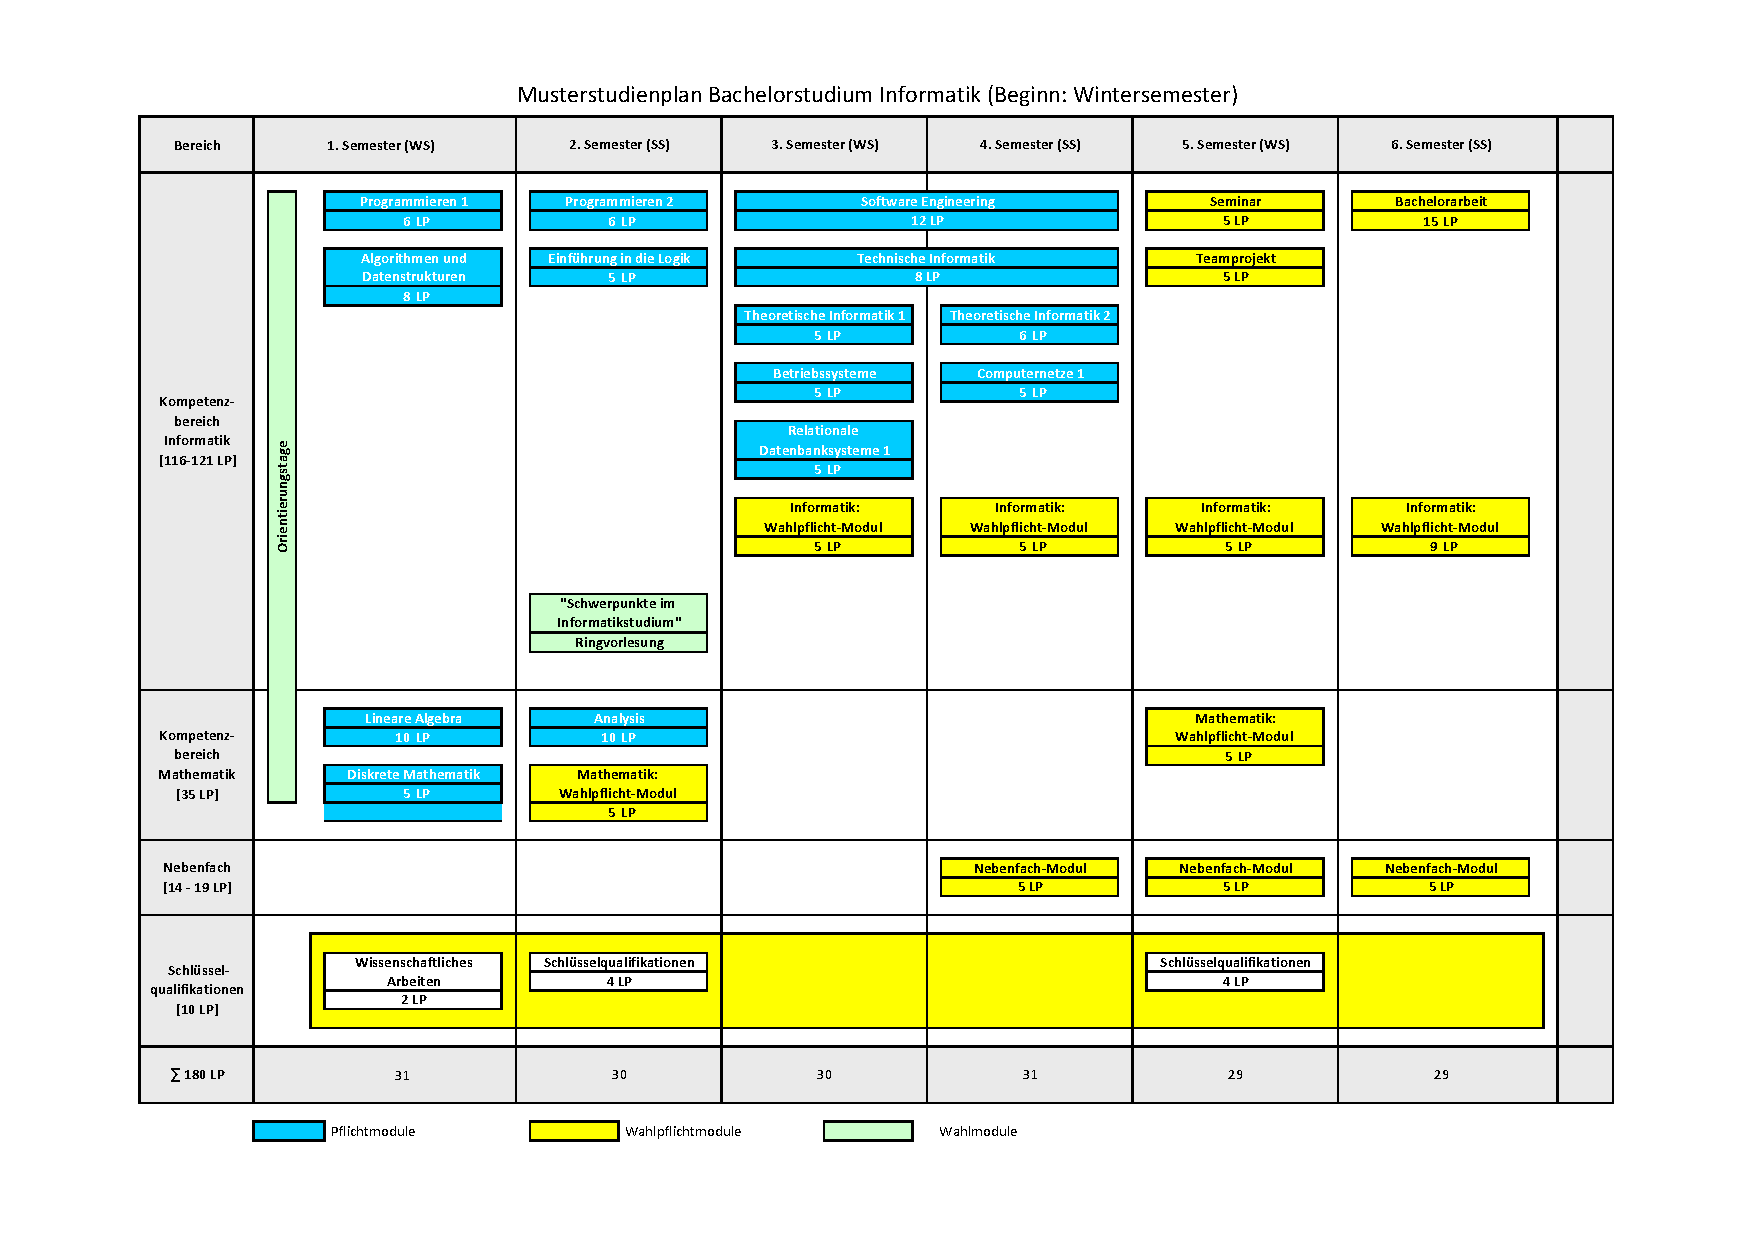
\includegraphics[angle=90,
totalheight=\textheight,
width=\textwidth ]{bilder/Musterstudienplan_BScInformatik_WS_02.pdf}
\end{center}  
\end{minipage}
\newpage
%\begin{minipage}{1.0\linewidth}
%\begin{wrapfigure}{r}{0.5\textwidth}   
%\newpage \
%\begin{center}     
%\newpage
%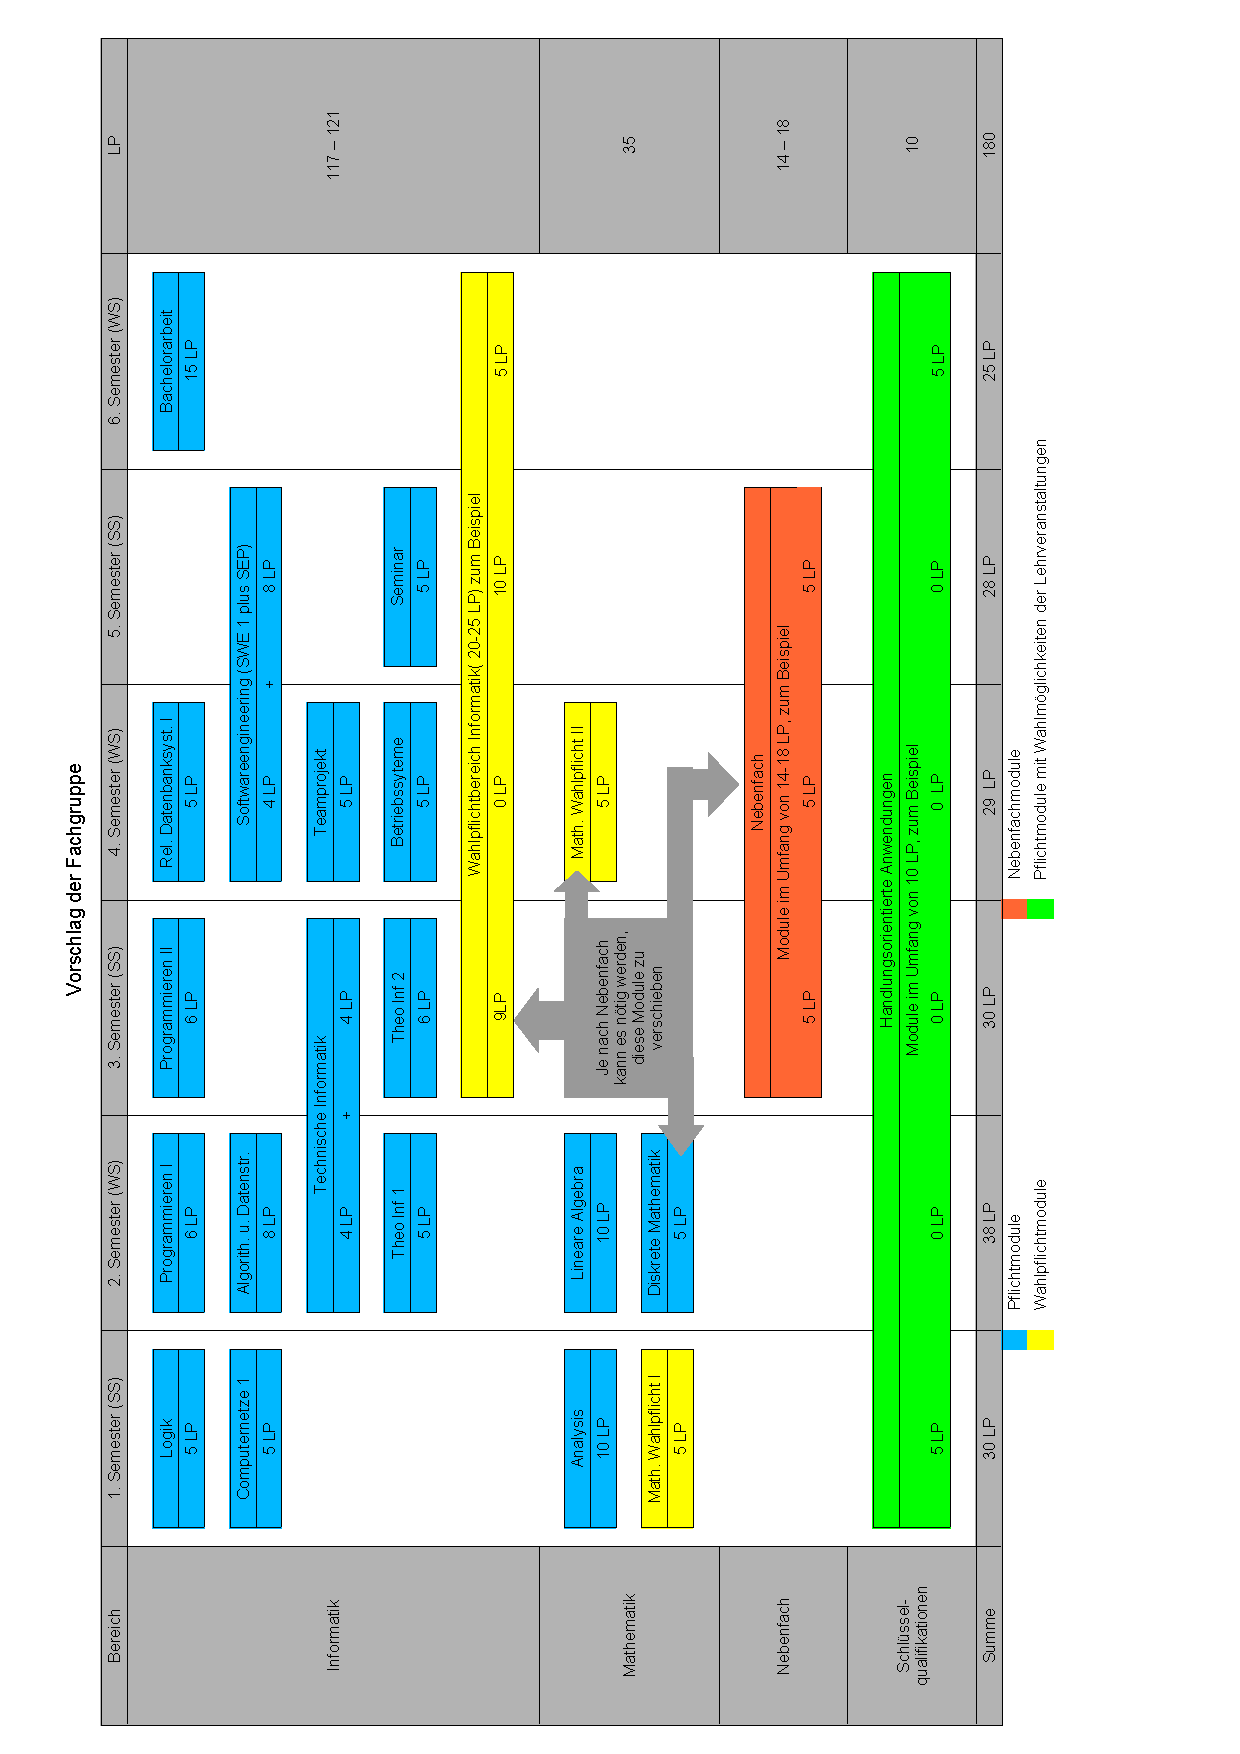
\includegraphics[totalheight=\textheight, width=\textwidth ]{bilder/FG_Vorschlag_BeginSS}
%\end{center}
%\end{wrapfigure}%\newpage  
%\label{studienplan_neu}
%\end{minipage} 
%\newpage
\begin{minipage}{1.0\linewidth}
%\newpage
 %Note that we have specified a size for b
%\begin{figure}[h!]
%\begin{wrapfigure}{r}{0.5\textwidth}  
\begin{center} 
  \centering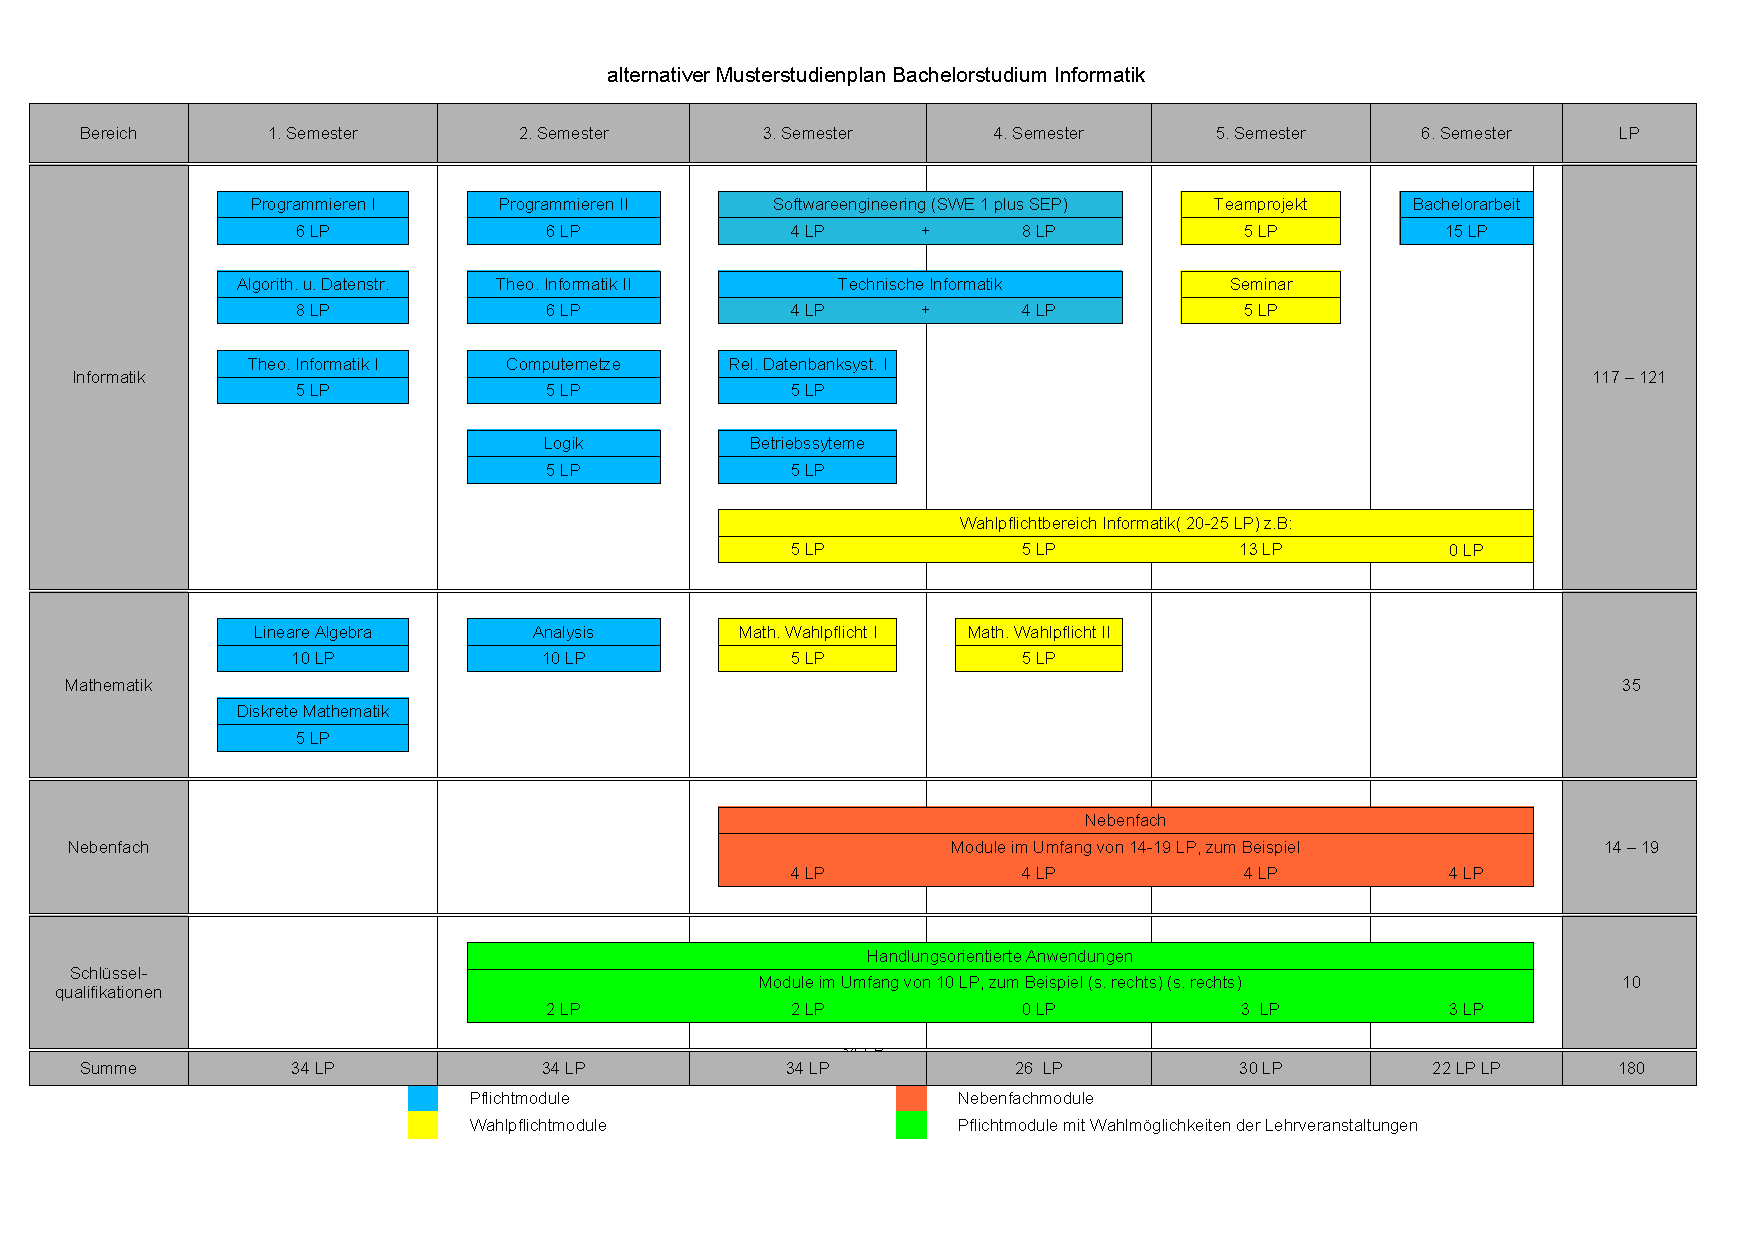
\includegraphics[angle=90,totalheight=\textheight,
  width=\textwidth ]{texte/bachelor/studienplan_neu.pdf}
\label{studienplan_neu}
\end{center}%\newpage
\end{minipage}
%\begin{figure}[h!]
  %\centering
\
\ %\newpage \ %\newpage 
\begin{multicols}{2}%\newpage

 %\newpage
\subsection{Studienplanung: Was alles schief gehen kann-
  Leidensbericht eines Fünftsemesters}
\label{studienplan_bericht}
  \textbf{WARNUNG: Dieser Text bezieht sich auf die alte
  Prüfungsordnung und den Studienbeginn im Wintersemester. Somit ist
  für euch nicht alles Weiteres übertragbar.}\\
Nun haben wir euch ja schon eine ganze Menge über die großen
Freiheiten bei der Studienplanung erzählt, sowie sogar noch einen
alternativen Plan vorgelegt. Nun fragt sich sicherlich der Eine oder
Andere, warum es nun noch mehr Text sein muss. Nun, wir dachten uns,
dass Planung gut und schön ist, aber nicht immer klappen muss. Also
dachten wir uns, dass wir am Beispiel eines mäßig begabten Studenten
das mal exemplarisch vorführen, inklusive angepassten
Studienplans. 
Ihr sollt ihr aus seinen Fehlern lernen, was man nicht machen sollte, aber
auch, wie man eigene Fehler noch korrigieren kann. Dazu schreiben wir
jedes Semester, was der Student vorhatte und was es dann geworden ist.
\subsubsection{Prolog}
Als ich anfing, hat uns die Fachgruppe neben der 1-ten uns
insbesondere ihren alternativen Musterstudienplan
\footnote{Die aktuelle Fassung für euch findet ihr auf Seite \pageref{studienplan_neu} - dieser Bericht bezieht sich natürlich 
auf die damalige Fassung für den Start im Wintersemester.}
ans Herz gelegt und
so nahm ich mir denn vor, brav danach zu gehen, aber alles kam ganz
anders...
\subsubsection*{1. Semester}

\newcommand{\nx}{\checkmark}

{
\footnotesize
\begin{tabular}{|l|r|c|c|}
\hline \textbf{Modul}		& \textbf{Credits} 	& \textbf{Plan} & \textbf{Real} \\ 
\hline
\hline Programmieren 1 		& 6 CP 				& \nx 			& \nx 	\\ 
\hline A. u. D.				& 8 CP 				& \nx 			& \nx 	\\ 
\hline Diskrete Mathematik 	& 5 CP 				& \nx 			& \nx 	\\ 
\hline Lineare Algebra 		& 10 CP 			& \nx 			& \nx 	\\ 
\hline Theo. Informatik 1	& 5 CP 				& \nx 			&  		\\ 
\hline Wissens. Arbeiten 	& 2 CP 				& \nx 			& \nx 	\\ 
\hline
\hline Summe 				&  					& 36 CP 		& 31 CP \\ 
\hline 
\end{tabular}
}

%Geplant:
%\begin{itemize}
%\item Programmieren 1 - 6 Credits
%\item Algorithmen und Datenstrukturen - 8 Credits
%\item Diskrete Mathematik - 5 Credits 
%\item Lineare Algebra - 10 Credits
%\item Theoretische Informatik 1 - 5 Credits
%\item Wissenschaftliches Arbeiten - 2 Credits
%\item Summe: 36 Credits
%\end{itemize}
Die Planung ging schon schnell nicht mehr auf, da ich noch damit
überfordet war, alle Hausaufgaben rechtzeitig und selbstständig zu
ersetzen. Insbesondere für Theoretische Informatik 1 war ich zu
unmotiviert und faul, und habe es dann nach den Weihnachtsferien
gekickt. Ich war dabei der Einzige der 5-6 Leute aus meinen Jahrgang,
die der Fachgruppenempfehlung gefolgt waren, alle anderen haben es
erfolgreich durchgezogen. Ich war also erst einmal gefrustet, vor
allem weil es für das Hören eines anderen Faches auch zu spät
war. Somit blieb alles beim offiziellen Musterstudienplan wie auf
Seite \pageref{musterstudienplan}:\\
%Geschafft:
%\begin{itemize}
%\item Programmieren 1 - 6 Credits
%\item Algorithmen und Datenstrukturen - 8 Credits
%\item Diskrete Mathematik - 5 Credits 
%\item Lineare Algebra - 10 Credits
%%\item Theoretische Informatik 1 - 5 Credits
%\item Wissenschaftliches Arbeiten - 2 Credits
%\item Summe: 31 Credits
%\end{itemize}

\subsubsection*{2. Semester}
{
\footnotesize
\begin{tabular}{|l|r|c|c|}
\hline \textbf{Modul}		& \textbf{Credits} 	& \textbf{Plan} & \textbf{Real} \\ 
\hline
\hline Programmieren 2 		& 6 CP 				& \nx 			& 	 	\\ 
\hline Technische Inf. 2	& 4 CP 				& \nx 			& 	 	\\ 
\hline Logik 				& 5 CP 				& \nx 			& \nx 	\\ 
\hline Computernetze 		& 4 CP 				& \nx 			& \nx 	\\ 
\hline Analysis 			& 10 CP 			& \nx 			& \nx	\\ 
\hline Stochastik 			& 5 CP 				& \nx 			& \nx 	\\ 
\hline \LaTeX\ 				& 3 CP 				& \nx 			& \nx 	\\ 
\hline
\hline Summe 				&  					& 37 CP 		& 31 CP \\ 
\hline 
\end{tabular}
}

Da mein Plan mit Theoretische Informatik 2 nicht aufging, musste ich
mir etwas anderes überlegen. Ich war nicht der Einzige und auf der
übrigens sehr empfehlenswerten Seite \url{http://www.clevershit.de/}
fragte jemand nach möglichen Fächern. Wir erfuhren, dass Technische
Informatik 2 trotz des Namens mit etwas Fleiß auch ohne Technische
Informatik 1 als Vorkenntnisse zu schaffen ist. Außerdem wollte ich
nach offiziellen Studienplan ein Mathewahlpflichtfach belegen. Zur
Auswahl standen Stochastik und Algebra. Ich entschied mich für
Stochastik. Dann habe ich  noch kurzfristig eine
Schlüsselqualifikation belegt, und zwar den Kurs ,,Einführung in die
wissenschaftliche Textverarbeitung mit \LaTeX\ '' \footnote{Der
  Anwendung verdankt ihr diesen Text ;)}.%\newpage 
Somit stand die oben gezeigt Planung für das zweite Semester fest.
%das Ergebnis war dann folgende Planung:
%\begin{itemize}
%\item Programmieren 2 - 6 Credits
%\item Technische Informatik 2 - 4 Credits
%\item Logik  - 5 Credits 
%\item Computernetze - 4 Credits
%\item Analysis - 10 Credits
%%\item Theoretische Informatik 1 - 5 Credits
%\item Stochastik - 5 Credits
%\item \LaTeX\ - 3 Credits
%\item Summe: 37 Credits
%\end{itemize}
Allerdings ging auch das nicht auf: Ich hatte in Technische Informatik
2 in der Tat keine Probleme der Vorlesung zu folgen, wenn ich denn mal
da war. Die Hausaufgaben für Stochastik, Programmieren 2, sowie Logik
forderten ihren Tribut und mein Vorlesungsbesuch wurde immer
sporadischer. Entsprechend bin ich dann durch die Prüfung
durchgefallen. Außerdem wollte ich eine gute Note in Analysis, da die
Gewichtung dort sehr stark ist. Entsprechend habe ich mich dann noch
von Programmieren 2 abgemeldet und übrig blieb folgendes:
%\begin{itemize}
%%\item Programmieren 2 - 6 Credits
%%\item Technische Informatik 2 - 4 Credits
%\item Logik  - 5 Credits 
%\item Computernetze - 4 Credits
%\item Analysis - 10 Credits
%%\item Theoretische Informatik 1 - 5 Credits
%\item Stochastik - 5 Credits
%\item \LaTeX\ - 3 Credits
%\item Summe: 27 Credits
%\end{itemize}

\subsubsection*{3. Semester}
{
\footnotesize
\begin{tabular}{|l|r|c|c|}
\hline \textbf{Modul}		& \textbf{Credits} 	& \textbf{Plan} & \textbf{Real} \\ 
\hline
\hline Technische Inf. 1 	& 4 CP 				& \nx 			& 	 	\\ 
\hline Technische Inf. 2 	& 4 CP 				& \nx 			& \nx	\\ 
\hline Relat. Datenb. 1 	& 4 CP 				& \nx 			& 	 	\\ 
\hline HS-Systeme 			& 4 CP 				& \nx 			& \nx	\\ 
\hline Betriebssysteme 		& 4 CP 				& \nx 			& 	 	\\ 
\hline Softwaretechnik 1 	& 4 CP 				& \nx 			& \nx	\\ 
\hline Theoretische Inf. 1 	& 5 CP 				& \nx 			& \nx 	\\ 
\hline Einf. in die Psych. 	& 5 CP 				& \nx 			& 	 	\\ 
\hline Geschichte der Math. & 5 CP 				& \nx 			& \nx	\\ 
\hline SQL-Praktikum		& 4 CP 				& 	 			& \nx 	\\ 
\hline
\hline Summe 				&  					& 39 CP 		& 26 CP \\ 
\hline 
\end{tabular}
}

Im dritten Semester musste ich nun also Theoretische Informatik 1 noch
einmal hören.  Außerdem musste ich ja noch die Klausur in Technische
Informatik 2 schreiben, weil ich diese ja (siehe oben) durch meine
Faulheit versemmelt hatte. Zudem musste ich mit den Nebenfach
anfangen. Ich entschied mich für Psychologie. Im
Schlüsselqualifikationsbereich fehlten mir nur noch 5 Credits. Da mir
eine Mitbewohnerin 
schon von der Vorlesung ,,Geschichte der Mathematik''  erzählt hatte,
und diese genau 5 Credits brachte ergab sich dann die oben gezeigte Planung.
%\begin{itemize}
%%\item Programmieren 2 - 6 Credits
%\item Technische Informatik 1 - 4 Credits
%\item Technische Informatik 2 - 4 Credits
%\item Relationale Datenbanken 1 - 4 Credits 
%\item Hardware-Software-Systeme - 4 Credits
%\item Betriebssysteme - 4 Credits
%\item Softwaretechnik 1 - 4 Credits
%\item Theoretische Informatik 1 - 5 Credits
%%\item Stochastik - 5 Credits
%\item Einführung in die Psychologie - 5 Credits \footnote{Dies ist
%    allerdings geraten, da zum Modul noch zwei andere Prüfungen
%    gehören. Die drei ergeben zusammen 10.}
%\item Geschichte der Mathematik- 5 Credits
%\item Summe: 39 Credits
%\end{itemize}
Natürlich kam es auch hier ganz anders als gedacht: Theoretische
Informatik 1 lief deutlich besser als erwartet, da doch noch
erstaunlich viel vom 1. Semester in Erinnerung geblieben war. Dafür
lief Technische Informatik 1 gar nicht. Spätestens, als unserer
Professor in Relationale Datenbanken, Herr Balke, uns vom
SQL-Praktikum erzählte, dass einen 4 Credits im Wahlpflichtbereich
Informatik einbringt, war mir klar, dass ich dafür Technische
Informatik 1 sausen lassen würde. Aus ähnlichen Gründen scheiterte
Betriebssysteme: Zwei Tage später musste ich Theoretische Informatik 1
schreiben und wieder zwei Tage später Relationale Datenbanken 1. Also
meldete ich mich von Betriebssysteme ab und hoffte so genug Zeit für
die anderen Prüfungen zu haben. Bei Theoretische Informatik 1 klappte
es, bei Datenbanken und Psychologie nicht. Dafür habe ich Technische Informatik 2 im
2. Versuch bestanden und somit blieb es bei 26 Geschafften Punkten.
%\begin{itemize}
%%\item Programmieren 2 - 6 Credits
%%\item Technische Informatik 1 - 4 Credits
%\item Technische Informatik 2 - 4 Credits
%%\item Relationale Datenbanken 1 - 5 Credits 
%\item SQL-Praktikum - 4 Credits
%\item Hardware-Software-Systeme - 4 Credits
%%\item Betriebssysteme - 5 Credits
%\item Softwaretechnik 1 - 4 Credits
%\item Theoretische Informatik 1 - 5 Credits
%\item Geschichte der Mathematik- 5 Credits
%\item Summe: 26 Credits
%\end{itemize}

\subsubsection*{4. Semester}
{
\footnotesize
\begin{tabular}{|l|r|c|c|}
\hline \textbf{Modul}		& \textbf{Credits} 	& \textbf{Plan} & \textbf{Real} \\ 
\hline
\hline Programmieren 2 		& 6 CP 				& \nx 			& \nx 	\\ 
\hline Betriebssysteme 		& 4 CP 				& \nx 			& \nx	\\ 
\hline Relat. Datenb. 1 	& 4 CP 				& \nx 			& \nx 	\\ 
\hline SEP 					& 8 CP 				& \nx 			& \nx	\\ 
\hline Theoretische Inf. 2 	& 6 CP 				& \nx 			&  		\\ 
\hline Chip- \& Systement. 1& 4\footnotemark[\value{footnote}] CP& \nx 		& 	 	\\ 
\hline Netzwerkalgorithmen	& 5 CP 				& \nx 			& \nx \addtocounter{footnote}{1}	\\ 
\hline Mensch im Kontext\footnotemark[\value{footnote}]& 5 CP	& \nx 			& 	 	\\ 
\hline
\hline Summe 				&  					& 42 CP 		& 27 CP \\ 
\hline 
\end{tabular}
}
\addtocounter{footnote}{-1}
\footnotetext[\value{footnote}]{Für den 1. Teil,
    also die Vorlesung plus Prüfung, der 2. Teil folgt im 5. Semester.} 
\addtocounter{footnote}{1}
\footnotetext[\value{footnote}]{Die Vorlesung heißt \textit{Der Mensch im sozialen Kontext/Das Individuum in seiner Entwicklung}. Die Creditzahl ist wieder geraten, da der 2. Teil
 des im 3. Semester angefangenen Moduls, beide ergeben zusammen 10} 
\addtocounter{footnote}{1}

So brach nun das vierte Semester an und somit das
Softwarentwicklungspraktikum (SEP). Nun freute ich mich darüber, schon
Computernetze und Technische Informatik 2 gemacht zu haben, blieb doch
als Pflichtfach nur Theoretische Informatik 2, und dazu noch zwei
Fächer aus der Psychologie, die den Rest des im WS angefangenen Moduls
bilden würden. Dazu kamen noch die Wahlmodule. Ich entschied
mich für Netzwerkalgorithmen, da ich Algorithmen und Datenstrukturen
vom 1. Semester noch in guter Erinnerung hatte. Aufgrund ähnlicher
Erfahrungen mit Hardware-Software-Systeme belegte ich außerdem die
Fortführung ,,Chip- und Systementwurf 1''.  Auch wollte ich endlich
die Klausuren für ,,Betriebssysteme'' und ,,Programmieren 2'', sowie
,,Relationale Datenbanken 1''
nachholen. 
%\begin{itemize}
% \item Programmieren 2 - 6 Credits
% \item Betriebssysteme - 4 Credits
%\item Relationale Datenbanken - 4 Credits
%\item SEP - 8 Credits
%\item Theoretische Informatik 2 - 6 Credits
%\item Chip- und Systementwurf 1 - 4 Credits \footnote{Für den 1. Teil,
%    also die Vorlesung plus Prüfung, der 2. Teil folgt im 5. Semester.}
%\item Netzwerkalgorithmen       - 5 Credits
%%\item Stochastik - 5 Credits
%\item Der Mensch im sozialen Kontext/Das Individuum in seiner Entwicklung - 5 Credits \footnote{Wieder geraten da der 2. Teil
%    des im 3. Semester angefangenen Moduls, beide ergeben zusammen 10}
%%item Geschichte der Mathematik- 5 Credits
%\item Summe: 42  Credits
%\end{itemize}
Mein Plan war also diesmal deutlich reduzierter, da ja ganze 14 Credits
erst zur Prüfungsphase relevant wurden. So dachte ich und so täuschte
ich mich. Das SEP erwies sich in der Tat als so zeitaufwendig und
stressig, wie höhere Semester immer berichtet hatten. Mit Müh und Not
schaffte ich daneben die Zulassung für Netzwerkalgorithmen und
Theoretische Informatik 2. Da ich insbesondere bei letzten Fach nicht
das Gefühl hatte, groß etwas verstanden zu haben, habe ich die Prüfung
dann lieber geschmissen und aufs 6. Semester vertagt. Dafür lief das
SEP und die ,,Altlasten'' unter den Prüfungen deutlich besser: Der
Betreuer war sehr angetan von unserer Arbeit und ich konnte endlich
ein Häkchen hinter Betriebssysteme, Programmieren und Datenbanken
setzen. Auch die mündliche Prüfung in Chip- und Systementwurf 1 lief
sehr gut, allerdings fehlt mir dazu noch das dazugehörige Praktikum. 
Offen bleibt  auch noch das
große Psychologiemodul, da ich ja den 1. Teil erst im Wintersemester
würde wiederholen können.
%\begin{itemize}
%%\item Programmieren 2 - 6 Credits
%%\item Technische Informatik 1 - 4 Credits
%%item Technische Informatik 2 - 4 Credits
%%item Relationale Datenbanken 1 - 5 Credits 
%%item SQL-Praktikum - 5 Credits
%%
%%\item Betriebssysteme - 5 Credits
% \item Programmieren 2 - 6 Credits
% \item Betriebssysteme - 4 Credits
%\item Relationale Datenbanken - 4 Credits
%\item SEP - 8 Credits
%%\item Theoretische Informatik 2 - 6 Credits
%%TODO: Anpassen nach CuSE Prüfung
%%\item Chip- und Systementwurf 1 - 4 Credits \footnote{Für den 1. Teil,
%%    also die Vorlesung plus Prüfung, der 2. Teil folgt im 5. Semester.}
%\item Netzwerkalgorithmen       - 5 Credits
%%\item Stochastik - 5 Credits
%%TODO
%%\item Psycholgoie - 5 Credits \footnote{Wieder geraten da der 2. Teil
%%   des im 3. Semester angefangenen Moduls}
%%item Geschichte der Mathematik- 5 Credits
%\item Summe: 27  Credits
%\end{itemize}

\subsubsection*{5. Semester}
{
\footnotesize
\begin{tabular}{|l|r|c|c|}
\hline \textbf{Modul}		& \textbf{Credits} 	& \textbf{Plan} & \textbf{Real} \\ 
\hline
\hline Seminar 				& 5 CP 				& \nx 			& 	 	\\ 
\hline Teamprojekt	 		& 5 CP 				& \nx 			& 		\\ 
\hline Numerik			 	& 5 CP 				& \nx 			& \nx 	\\ 
\hline Prakt. Chipentwurf	& 6 CP 				& \nx 			& \nx	\\ 
\hline Verhalten \& Prozesse\footnotemark[\value{footnote}]& 6 CP	& \nx 			& \nx	 	\\ 
\hline Einf. in die Psych. 	& 5 CP 				& \nx 			& \nx	\\ 
\hline
\hline Summe 				&  					& 36 CP 		& 22 CP \\ 
\hline 
\end{tabular}
}
\footnotetext[\value{footnote}]{Gesetzmäßigkeiten von Verhalten und mentalen Prozessen} 

%Dazu kommen noch die 4 Credits des ersten Teils vom Chipentwurf
%sowie die 5 Credits aus den Psycholgievorlesungen im 4. Semester,
%also insgesamt 45 Credits.

Fürs fünfte Semester lag nun einiges vor mir: Zum einen das Seminar
und das Teamprojekt. Zum anderen wollte ich nun 
endlich Technische Informatik 1, sowie meine versemmelte Psycholgieklausur nachholen. Außerdem fehlt mir
noch das 2. Mathe-Wahlpflichtmodul (ich entscheide mich für Numerik), sowie  das Praktikum für Chip-
und Systementwurf 1. Im Psychologie fehlt mir dann noch das Modul ,,Gesetzmäßigkeiten von Verhalten und mentalen Prozessen'':
%Außerdem fehlen mir noch 4 Credits im Informatik Wahlpflichtbereich,
%aber es wird ja genug angeboten :)
%\begin{itemize}
%\item Technische Informatik 1 - 4 Credits
%\item Seminar - 5 Credits
%\item Teamprojekt - 5 Credits
%\item Numerik - 5 Credits
%\item Praktikum zum Chipentwurf - 6 Credits
%%\item Wahlpflichtmodul Informatik - 4 Credits
%\item Gesetzmäßigkeiten von Verhalten und mentalen Prozessen - 6
%  Credits
%\item Einführung in die Gebiete der Psychologie - 5 Credits (bereits
%  im 3. Semester gehört, damals aber durchgefallen)
%%\item SEP - 8 Credits
%\item Summe: 36 Credits
%\item Dazu kommen noch die 4 Credits des ersten Teils vom Chipentwurf
% sowie die 5 Credits aus den Psycholgievorlesungen im 4. Semester,
% also insgesamt 45 Credits.
%\end{itemize}
Damit hatte ich mich wieder mal ziemlich verhoben. Ganz gut liefen
dabei noch das Chipentwurfspraktikum, sowie Numerik. Während das
Praktikum einfach Spass machte, war Numerik endlich mal ein einfaches
Mathefach. Auch die Psychologievorlesungen waren mal wieder sehr
interessant, auch wenn ich längst nicht immer da war.  Das Seminar und
das Teamprojekt forderten ihren Tribut, auch wenn beide letzlich nicht
ganz liefen wie gewünscht. Zum Seminarthema fand ich erst keinen
Zugang und am Ende konnte ich das nicht mehr aufholen, weshalb ich es
dann geschmissen habe. Auch das Teamprojekt zog sich ziemlich hin. Wir
hoffen nun, dass wir es in April abschließen werden, also im neuen
Semester. Bei der technischen Informatik rächte sich schließlich meine
Faulheit und es hatte sich mal wieder eine versemmelte Klausur mehr angesammelt.
Von den vorgenommenen 45 Credits habe ich nur einen Bruchteil geschafft.
%\begin{itemize}
%\item Numerik: 5 Credits
%\item Praktikum zum Chipentwurf - 6 Credits
%%\item Wahlpflichtmodul Informatik - 4 Credits
%\item Gesetzmäßigkeiten von Verhalten und mentalen Prozessen - 6
%  Credits
%\item Einführung in die Gebiete der Psychologie - 5 Credits (bereits
%  im 3. Semester gehört, damals aber durchgefallen)
%\item Summe: 22 Credits 
%\end{itemize}
Immerhin war damit mein Nebenfach und Chip- und Systementwurf 1
abgeschlossen, dass ich immerhin insgesamt noch 31 Credits verbuchen
konnte.

\subsubsection*{6. und 7. Semester}
{
\footnotesize
\begin{tabular}{|l|r|c|}
\hline \textbf{Modul}		& \textbf{Credits} 	& \textbf{Plan} \\ 
\hline
\hline Technische Inf. 1 	& 4 CP 				& \nx 			\\ 
\hline Theoretische Inf. 2 	& 6 CP 				& \nx 			\\ 
\hline Seminar				& 5 CP 				& \nx 			\\ 
\hline Teamprojekt 			& 5 CP 				& \nx 			\\ 
\hline 
\hline Bachelorarbeit 		& 15 CP 			& \nx 			\\ 
\hline 
\hline Summe 				&  					& 20 / 15 CP 		\\ 
\hline 
\end{tabular}
}

Auch wenn es schon den Ende entgegen geht, hat sich doch einiges noch
angesammelt, sodass ich die Bachelorarbeit erst im 7. Semester
schreiben werde. Vorher aber muss
ich noch meine letzten Scheine schaffen.
%\begin{itemize}
%\item Sechstes Semester:
%\item
%  \begin{itemize}
%  \item Technische Informatik 1 - 4 Credits
%  \item Theoretische Informatik 2 - 6 Credits
%  \item Seminar: 5 Credits
%  \item Teamprojekt 5 Credits
%  \item Summe: 20 Credits
%  \end{itemize}
%\item Siebtes Semester
%  \begin{itemize}
%  \item Bachelorarbeit: 15 Credits
%  \end{itemize}
%\end{itemize}

% Wenn alles nach Plan klappt, habe ich im 6 Semester also nur noch 21
% Credits zu absolvieren, nämlich 6 für Theoretische Informatik 2, sowie
% 15 Credits für die Bachelorarbeit. 
Da ich in der theoretischen
 Informatik starke Defizite habe, werde ich die Vorlesung wohl nochmal
 hören. Dazu kommt noch das Seminar und der Abschluss des
 Teamprojektes und die Klausur in technischer Informatik 1. Um dort
 nun keine weiteren Verzögerungen zu kriegen, ist die Bachelorarbeit
 also noch in weiter Ferne. Aufmerksamen Lesern wird auffallen, dass
 mir noch Credits fehlen. Dazu muss man wissen, dass ich nach der
 alten Prüfungsordnung studiert habe und einige der Fächer mit 4
 Credits durch einen Prüfungswechsel noch aufgewertet werden, das habe
 ich im Text noch nicht berücksichtigt.\\
Insgesamt hat sich mein Studienplan also
 ganz anders entwickelt als gewünscht.
 % Ihr findet ihn als mahnendes
% Beispiel auf Seite \pageref{studienplan_irre}.
% Meine Erfahrung sagt mir aber, dass wohl auch diese Planung
% wieder nicht ganz hinhauen wird. Andererseits ist man flexibel und es
% ist ja nicht das erste Mal, dass ich Fächer in Studienplan hin und her
% schiebe und somit aus einer blöden Situation noch das beste raus
% hole. Den sich daraus ergebenden Studienplan sieht ihr auf der
% nächsten Seite. 
%  Auch sind meine Angaben beim Nebenfach und den
% Wahlfächern natürlich die, die ich belegt habe und somit natürlich nur
% ein Vorschlag.
\paragraph{Nachbemerkungen}
Diese Geschichte ist mir wirklich so passiert und auch noch nicht
abgeschlossen. %Den derzeitigen sich daraus ergebdenen Studienplan
%findet ihr nun auf der nächsten Seite.
 Die eigentliche Frage ist: Warum steht sie hier? Egotrip des
Autors? Darstellen, wie sch*e alles ist? Zeigen, dass Studenten
manchmal sehr ,,verplante'' Studenten sein können?\\\\
Nun, von allen ein Bisschen, der Hauptsinn ist aber ein Anderer: Diese
kleine Geschichte soll zeigen, dass wirklich nichts fest ist im
Bachelor und man grundsätzlich alles umlegen kann wie man will. Ich
kann meinen Studienplan in der Form übrigens nicht zur Nachahmung
empfehlen, da die Belastung pro Semester stark ungleichmäßig verteilt
ist.  Außerdem gilt für euch eine neue Prüfungsordnung mit anderer
Modulstruktur. Er soll aber zeigen, dass wenn etwas schief geht, man trotzdem
noch etwas retten kann, indem man ein wenig hin und her schiebt. Als
Vorlage eignet er sich trotzdem nicht, da für euch schon ein anderes
Modulhandbuch gilt, und deshalb einige Dinge so wohl nicht mehr
möglich sind (welche standen zum Redaktionsschluß noch nicht
fest). Auch muss ich zugeben, dass der Text nicht ohne Weiteres
verständlich ist. Für
Rückfragen  kann man sich aber gerne bei mir  melden. Die Geschichte ist
auch noch nicht abgeschlossen und dieser Text wird für die nächste
1-te sicherlich noch einmal umgeschrieben. Verbesserungsvorschläge und
weiteres Feedback nehme ich daher  gerne entgegen.\\
\emph{Johannes Starosta -- \nolinkurl{J.Starosta@tu-bs.de}}
%\end{multicols}%\newpage
%\begin{figure}[p]
%  \centering
%\label{studienplan_irre}
%  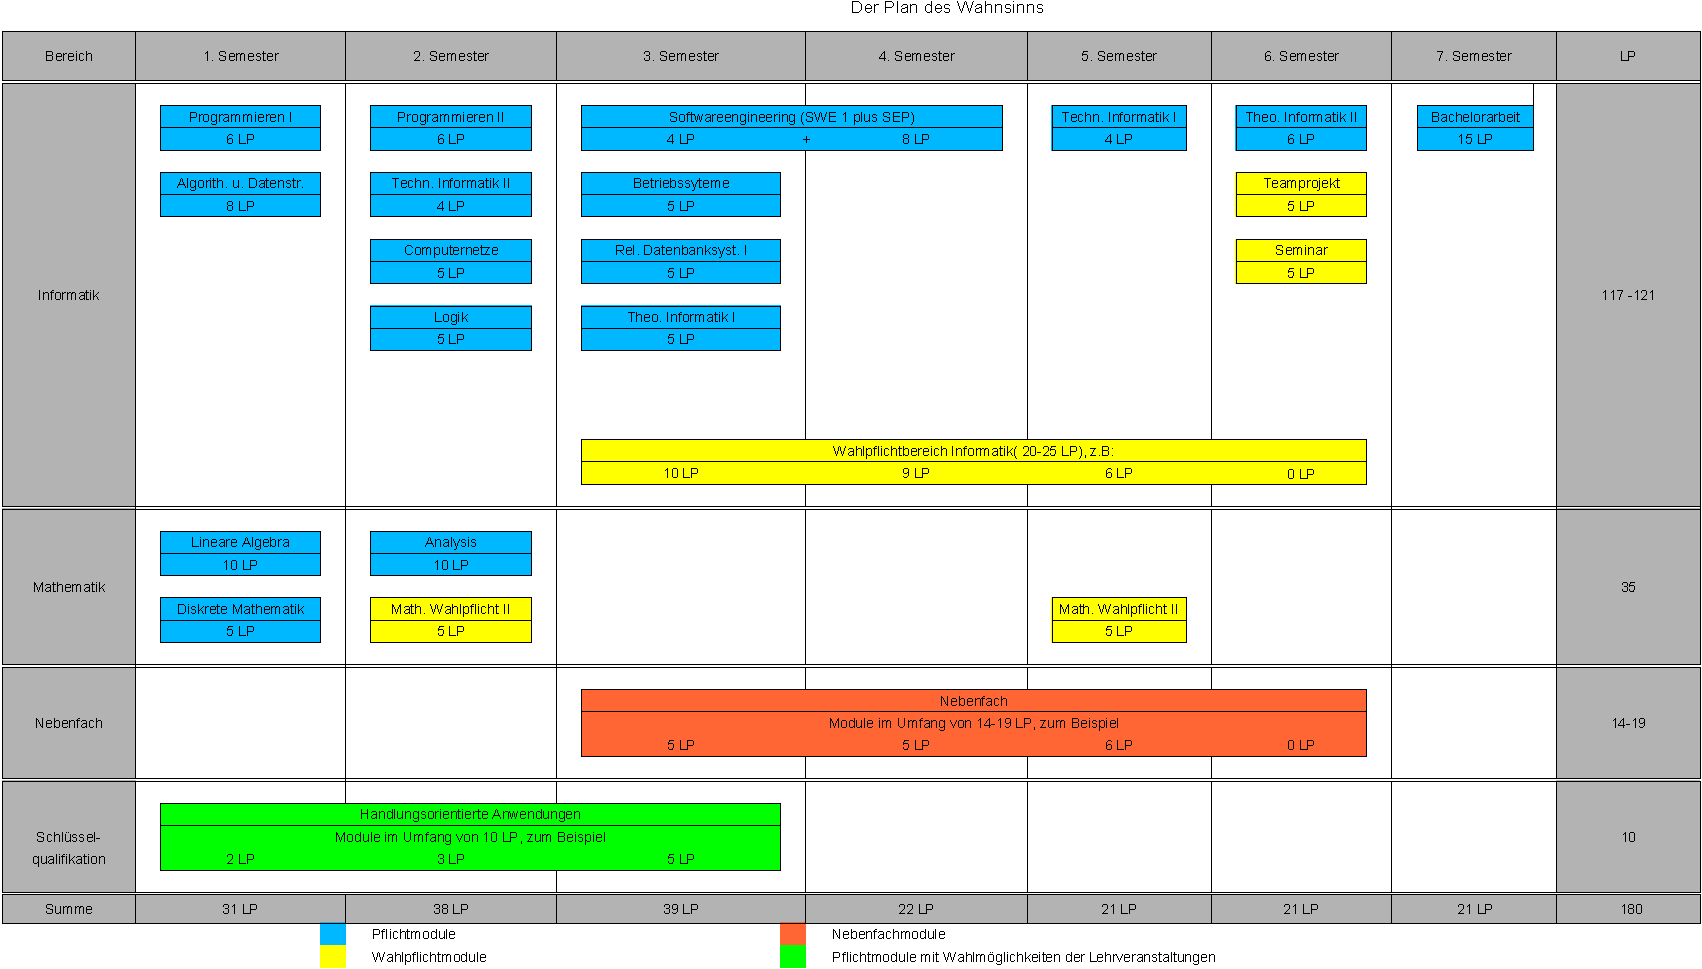
\includegraphics[angle=90,width=0.9\textwidth ]{texte/bachelor/studienplan_joke.pdf}
%\end{figure}
%\begin{multicols}{2}
 % d
%%% Local Variables: 
%%% mode: latex
%%% TeX-master: "../../1-te"
%%% End: 

%%% Local Variables: 
%%% mode: latex
%%% TeX-master: "../../1-te"
%%% End: 
 %Import mit Seitenumbruch
	% !TEX root = ../../1-te.tex

\begin{minipage}{1.0\linewidth}
	\begin{center}     
 		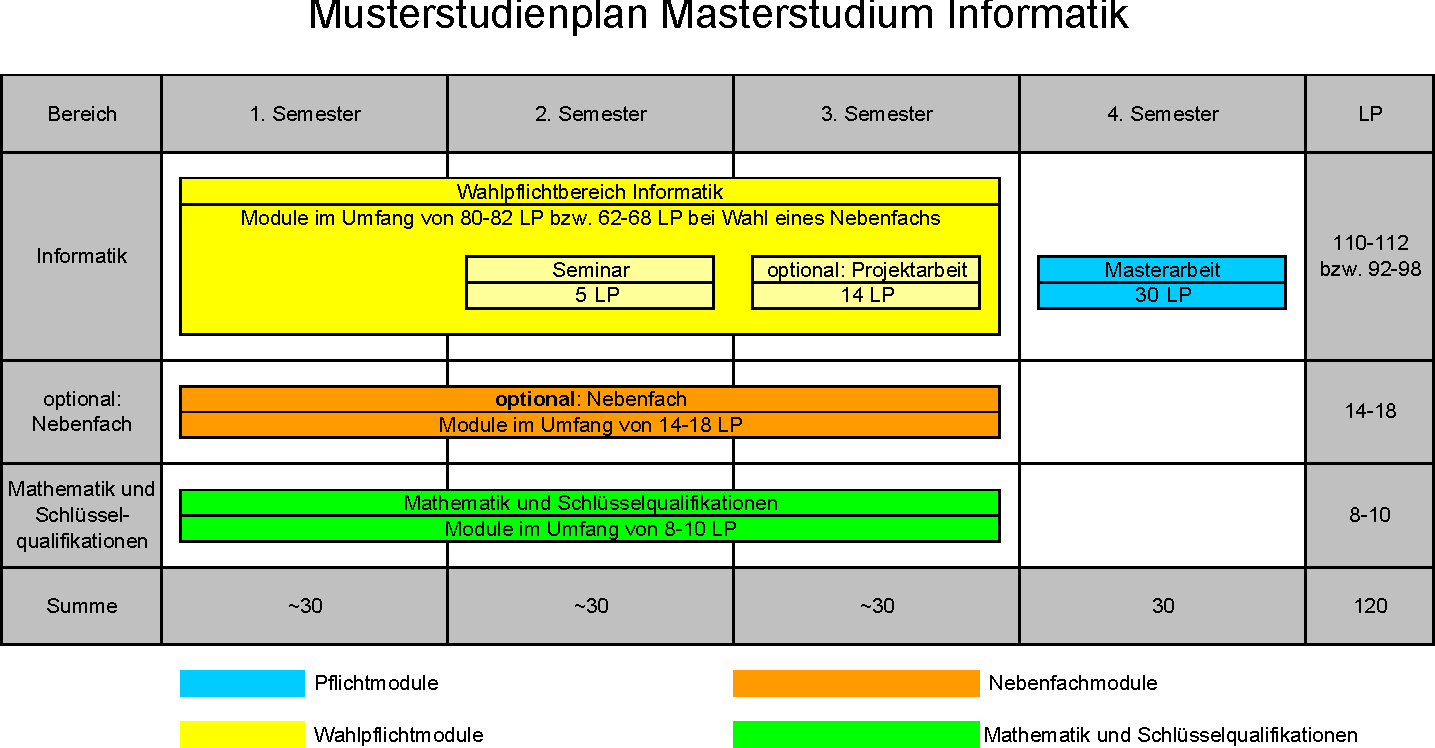
\includegraphics[width=\textwidth]{bilder/studienplan_msc/Musterstudienplan_MSc.pdf}
	\end{center} 
\end{minipage}

\begin{multicols}{2}
	Wer seinen Bachelor nicht in Braunschweig erworben hat, steht im ersten Mastersemester vielen kleinen und mittelgroßen Schwierigkeiten gegenüber.

	\subsection{Unterschiede zwischen den Bachelor-Abschlüssen}
		Eventuell hat dein bisheriger Abschluss dir mehr als 180 Credit Points eingebracht -- genau so viele hättest du nämlich in einem Bachelor an dieser TU erreicht. Es ist theoretisch möglich, solche überschüssigen CPs auf den Master anzurechenen, wenn man von seiner alten Hochschule bestätigt bekommt, dass sie für den Bachelor nicht verwendet wurden. Dann kann man die Anerkennung dieser CPs beim Prüfungsausschuss beantragen, wobei man möglichst schlüssig begründen muss, warum diese Vorlesungen dem TU-BS-Master würdig sein sollen.

		Selbst bei gleicher Anzahl an CP ist der Bachelor an jeder Hochschule ein wenig anders. Zwischen Universitäten in Deutschland herrscht eine formale Übereinkunft über die Inhalte des Bachelor-Studiums Informatik. 

		Falls du von einer Nicht-Universität (z.B. Fachhochschule) oder aus einem Studiengang der nicht exakt \emph{Informatik} heißt kommst oder dein Abschluss kein Bachelor of Science ist, dann kann es durchaus sein, dass du bei gewissen Unterschieden Zulassungsauflagen bekommst, um diese zu beheben.

	\subsection{Zulassungsauflagen}
	\label{auflagen}
	Ob du Zulassungsuflagen bekommst, steht in einem der ersten Briefe, die du von der TU erhältst, heb diesen Brief gut auf! Wenn du keine solchen Zulassungsauflagen hast, kannst du diesen Abschnitt überspringen.

	Es handelt sich dabei um Fächer aus dem Informatik-Bachelor, die du zusätzlich zu den Master-Fächern belegen musst -- sie gehen aber nicht in die Masternote oder CP ein und müssen innerhalb des ersten Jahres bestanden und im I-Amt nachgewiesen werden, sonst droht die Exmatrikulation.

	Der Sinn hinter den Auflagen ist es, Differenzen zum TU-BS-Bachelor auszugleichen, d.h. Inhalte nachzuholen, die in deiner bisherigen Ausbildung zu kurz kamen oder ganz fehlten, und hier wichtige Grundlage des Masterstudiums sind.

	Es ist möglich, zu Semesterbeginn freiwillig an einer mündlichen Prüfung teilzunehmen. Wird diese bestanden, dann ist die Auflage erfüllt, falls nicht, muss wie gehabt die Klausur belegt werden. Auch wird in den meisten Fächern die Hausaufgabe nicht mehr verpflichtend sein, um an der Klausur teilzunehmen.

	Viele Fragen zu den Zulassungsauflagen sind unter \fginfoUrl $\rightarrow$ FAQ dokumentiert und nach bestem Wissen und Gewissen beantwortet. Falls du eine Auflage erhalten hast, die dir fragwürdig erscheint oder du sonst irgendwelche Fragen dazu hast, wende dich am besten an den Fachgruppenrat.

	Ratsam ist es auch, mit den anderen Ersties in deinem Jahrgang zu sprechen und zu vergleichen, wie deren Auflagen aussehen bzw. welche Schritte diese gerade erwägen. 

	\subsection{Selbstständiges Nachlernen von Bachelor-Fächern}
		Vielleicht hat dein Bachelor eine andere Ausrichtung gehabt als die TU und somit in manchen Bereichen klare Wissenslücken hinterlassen. Wenn du das Gefühl hast, dass dir Wissen fehlt, das im Braunschweiger Bachelor vermittelt wurde, kannst du dich natürlich auch freiwillig in jede Bachelor-Vorlesung oder Übung hineinsetzen -- Punkte gibts dafür normalerweise keine. Aber egal was dir aus dem Bachelor fehlt, es finden sich eigentlich genug Master-Fächer, die auch ohne bestimmte Vorkenntnisse, gut schaffbar sind. Einige wenige Master-Vorlesungen beginnen auch mit einer mehrwöchigen Widerholung der Bachelor-Grundlagen. Im Zweifelsfall frage Studierende aus den höheren Semestern oder den oder die Professor/in selbst, welche Vorkenntnisse man wirklich braucht.

	\subsection{Der eigene Stundenplan}
		\label{masterstundenplan}
		Es gibt durchaus Studierende, die mit dem Stundenplanbau kein Problem haben: Sie schauen einige Minuten auf den Gesamstundenplan, es macht Klick, und sie wissen, welche Fächer sie belegen wollen. Andere verbringen bis zu 12 Stunden damit ihren Stundenplan zu bauen.

		Wenn du Zulassungsauflagen hast, haben diese oberste Priorität. Die entsprechenden Vorlesungen und Übungen kannst du ohne großes Nachdenken in deinen Stundenplan eintragen -- außer wenn du die freiwillige mündliche Prüfung bestanden hast.

		Danach kannst du probieren den allgemeinen Stundenplan pro Block durchzugehen und zu entscheiden, welches der dort stattfindenen Fächer für dich interessant klingt. Wenn du so vorgehst, hast du vermutlich am Ende einen Plan mit viel zu vielen Fächern, also deutlich mehr als 30 Credit Points. Und was zu Beginn noch überschneidungsfrei aussieht, kollidiert am Ende vielleicht bei den Übungsterminen. 

		Man muss nicht immer beide Veranstaltungen besuchen: bei manchen Fächern kann man die Übung getrost weglassen, oder den Stoff auch ohne Vorlesung aus Skript und Büchern lernen und nur zur Übung kommen. Manche Institute filmen ihre Vorlesungen auch und machen sie terminunabhängig. Frage am besten höhere Semester nach ihren Erfahrungen mit dem betreffenden Fach.

		\vspace{0.5cm}
		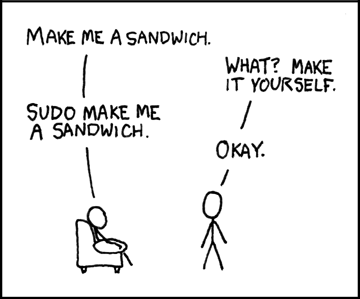
\includegraphics[totalheight=6cm]{bilder/XKCD/sandwich}
	\subsubsection{Hilfe beim Stundenplanbau}
		\tocheck{3}{Wann findet der Workshop diese Jahr statt?}
		Wir bieten seit einigen Semestern zu Beginn Hilfe beim Stundenplanbau an. Dieses Mal findet der Workshop am Mittwoch in der O-Woche um 12:30 Uhr statt. 
\end{multicols}
 
	\section{Computer und so\ldots}
	\label{computer}

\begin{multicols}{2}
	\emph{Informatik hat viel mit Computern zu tun!} - Diesem (Irr-)glauben erliegen zu Anfang des Studiums einige, auch wenn sich inzwischen öfter rumspricht, dass das Studium abstrakter sein kann. Das Informatikstudium ist nicht dafür da,  euch beizubringen, wie man einen Computer bedient. Somit sind diese Seiten eventuell das erste und letzte Mal,  dass euch Infos zu diesem Thema direkt vorgesetzt werden. Natürlich können wir hier nur ein paar Tipps geben und euch darauf hinweisen, wo ihr mehr Infos  findet.

	In Wirklichkeit hängt es seht von deiner Spezialisierung im Studium ab, ob  du den Computer im Studium mehr brauchen wirst als ein Student der Germanistik oder Sozialwissenschaften. Denn die einzigen Inhalte,  die jeder direkt am Rechner lernen und umsetzen muss, sind die Hausaufgaben,  die in Programmieren aufgegeben werden, sowie später noch das SEP und das Teamprojekt. Den Rest der Informatik kannst du evtl. komplett auf dem Papier absolvieren.

	Dennoch sind Computer ein unersetzliches Werkzeug um durchs Studium zu kommen. Und je nach den von dir gewählten Modulen kann sich das oben gesagte auch ins Gegenteil verkehren, so dass du mehr Zeit vorm Rechner als im Bett verbringst.

	Aber heißt dass nun, dass ihr um zu Studieren einen eigenen, top-aktuellen Rechner braucht, und dass ihr absolute PC-Freaks sein solltet? Dem wollen wir auf den nächsten Seiten ein wenig auf den Grund gehen.
\end{multicols}

%\begin{multicols}{2}
	\subsection{Wozu Computer?}
		\subsubsection{Vorlesungen Online}
			Zu den meisten Vorlesungen kann man die Skripte im Internet finden. Für einige Vorlesungen gibt es sogar Ton- oder Videomitschnitte.

			Es gibt auch immer engagierte Studierende, die ihre Vorlesungsmitschriften online stellen. Da diese sehr wahrscheinlich in deinem Semester sind, hilft es, wenn du dich in den Vorlesungen umhörst. Ansonsten ist \url{https://www.clevershit.de} die richtige Anlaufstelle für den Informationsaustausch zwischen Studenten.

		\subsubsection{Organisatorisches ohne Papier}
			Ansonsten gibt es eine Reihe von Informationen, die man nur über das Web bekommt, und mehr und mehr Formalitäten (z.B. die Prüfungsanmeldung) werden auch in die virtuelle Relatität verlagert.

			Desweiteren kannst du dir im Netz einen individuellen Stundenplan zusammenstellen, in Erfahrung bringen, wann die nächsten Klausuren stattfinden, lesen, was es in der Mensa zu essen gibt, endlich herausfinden, wann das Prüfungsamt geöffnet hat,  offene HiWi"~Stellen bei den Instituten finden und vieles mehr.

			Die Webseiten der TU sind ein großer Dschungel, durch den man sich am besten  mit Machete und Googlesuche kämpft. Um an der TU etwas zu finden, solltest du deinem eigentlichen Suchbegriff wahlweise \enquote{tu braunschweig} oder \enquote{site:tu-braunschweig.de} anhängen, und schon hast du gute Chancen zum Ziel zu kommen.

		\subsubsection{Mitschreiben am PC}
			Auf den ersten Blick mag es naheliegen, sich
			während der Vorlesungen Notizen  am Laptop
			anzufertigen. In der Praxis gibt es da aber eine
			Reihe von Problemen, vor denen wir  warnen
			möchten. Es hat schließlich seinen Grund, das
			nur 10\% der Studenten in der Vorlesung am
			Laptop sitzen und davon 90\% diesen nur nutzen,
			um zu zocken: Die meisten Tafelanschriften
			bestehen  aus verschachtelten Formeln,
			fremdartigen Buchstaben und verworrenen
			Zeichnungen. Diese in Echtzeit in den Laptop
			einzuhacken ist eine besondere Kunst, die du mit
			Notepad und Word gar nicht erst probieren
			brauchst. Eine Chance hast du vielleicht mit
			einem Tablet PC, oder wenn du
			\LaTeX\ bereits im Schlaf beherrscht -
			aber wer tut das schon zu Beginn des Studiums?

			In den Vorlesungen, in denen du nicht Tafelweise abschreiben musst, sondern nur hier und da mal etwas notieren, zeigt sich der PC schon als nützlicher. Wenn du ab und zu den Vortrag des Profs damit vergleichen möchtest, was er in sein Skript geschrieben hat, kann dir der mitgebrachte Laptop unter Umständen das Ausdrucken von ein paar hundert Seiten ersparen. Du wirst aber schnell merken, dass es in praktisch keinem der Hörsääle und Seminarräume Steckdosen gibt, und in manchen nichtmals ausreichende WLAN-Signalstärke.

		\subsubsection{Hausaufgaben am PC}
			In vielen Fächern musst du regelmäßig
			Hausaufgaben erledigen und einreichen. Keiner
			erwartet von dir, dass diese mit dem PC gemacht
			werden, es ist also völlig ok sie von Hand zu
			schreiben. Es hat aber auch gewisse Vorteile,
			sie am PC zu schreiben (z.B. mittels \LaTeX) und
			dann auszudrucken. Bei \LaTeX\ handelt es sich
			um ein Satzsystem für wissenschaftliche
			Texte wie Haus- oder Abschlussarbeiten.
			Erwähnenstwert ist die hervorragende
			Unterstützung für den Satz mathematischer
			Formeln und dass dabei mit Befehlen, ähnlich wie
			in HTML gearbeitet wird. Es gibt \LaTeX-Kurse die du im Schlüsselqualifiktationsbereich anrechnen lassen kannst, aber mit den Infos im WWW kann man sich das auch selbst beibringen. Je eher du damit anfängst, desto weniger Probleme hast du später, wenn du damit z.B. deine Abschlussarbeit aufsetzt.

		\subsection{Computer-Pools an der Uni}
			Es ist immer nützlich zu wissen, wo man mal schnell an einen Computer kann. Zumindest ab und zu wirst du die Computer in der Uni benutzen, besonders die Linuxarbeitsplätze in \textbf{PK4.5} oder \textbf{PK4.8}, an denen du die Hausaufgaben für Programmieren abgeben musst.

			\begin{itemize}
				\item[*] Im Erdgeschoss des Altbaus gibt es auf der rechten Seite zwei Computerräume, einen weiter vorne (\textbf{PK4.6}) und einen genau in der Ecke des Gebäudes (\textbf{PK4.5}). Zwei weitere Räume (\textbf{PK4.8} und die \textbf{Datenstation}) findest du im ersten Stock des Altbaus, auch wieder in der rechten Ecke. Die Rechner in \textbf{PK4.5} und \textbf{PK4.8} sind mit Linux ausgestattet. Im ersten Stock gibt es nun auch einen Windowsrechnerraum. Da kann man mal eine Word- oder Powerpoint-Datei ausdrucken, wenn man denn muss.

				\item[*] Reichlich Computer findet man schließlich im Gauß-IT-Zentrum~(GITZ) an der Hans-Sommer-Straße. Das ist der gedrungene, fast würfelförmige, dunkle Klotz hinter dem Elektrotechnik-Hochhaus (\emph{E-Tower}). Hier gibt es mehrere frei zugängliche Räume mit  Linux- und Windowsrechnern. Es gibt hier auch Räume für Medienbearbeitung, wo du etwa Video-Digitalisierer, ein Tonstudio und Rechner mit der Adobe Creative Suite Production Premium nutzen kannst.

				\item[*] Seit 2010 stellt das IBR (Institut für Betriebssysteme und Rechnerverbund) im Raum G40 des Informatikzentrums einen Rechnerraum mit vielen, schnellen Linux-Rechnern  zur Verfügung. Zu diesem CIP-Pool (Computer-Investitions-Programm) bekommt man mit seiner y-Nummer Zutritt. Wenn man Glück hat, funktioniert sogar einer der beiden Drucker in diesem Raum, so dass man zum Drucken nicht das IZ verlassen muss.
			\end{itemize}

		\subsection{Der eigene Rechner}
			Wenn du trotz aller Widrigkeiten planst, dir
			extra für's Studium einen (tragbaren) Rechner
			anzuschaffen, dann hast du hier gleich ein wenig
			Kaufberatung: Viel (Rechen- bzw.
			Grafik-)Leistung brauchst du im Studium  nur für
			sehr wenige spezielle Fachgebiete - das
			einfachste Netbook wird also vermutlich schon
			reichen. Wichtiger ist vielmehr die Akkulaufzeit
			und die WLAN-Empfangsstärke. %a die Här	

		\subsubsection{Welches System?}
			Dir wird auffallen, dass zwar alle Systeme geduldet sind, aber die Linux hier deutlich öfter über den Weg laufen wird als in der freien Wildbahn. Auch wir sind große Linux-Fans und haben deshalb ab Seite \pageref{linux} ein paar Infos dazu zusammengetragen.

			Aber trotz dieser nicht ganz unauffälligen Beeinflussung gilt: Beim Betriebssystem hast du freie Wahl. Sämtliche Software, die du für's Studium brauchen  könntest, gibt es für alle großen Systeme, meist sogar gratis. Für Linux ist eh  praktisch alles frei erhältlich, für Windows spendiert Microsoft den Studenten auch alles außer Office (siehe Seite \pageref{msdnaa}), und auch Apple bringt dich dank satter Studentenrabatte durch Bachelor und Master. 

		\subsubsection{Wege ins Uni-Netz}
			Um den eigenen Rechner ins Netz zu bekommen, stehen die in der Uni WLAN und LAN offen. Zur Konfiguration siehe Seite \pageref{wlan}.

			Für manche Aktivitäten (z.B. den Zugriff auf Prüfungsprotokolle) musst du dich direkt im Uni-Netz befinden. Wenn du und dein Rechner aber gerade zuhause oder sonstwo sind, heißt dass nicht, dass du dich nun physisch auf den Weg machen musst. Mittels VPN kannst du dich virtuell ins Uni-Netz einklinken. Schau einfach mal auf den Seiten des GITZ nach, um mehr zu erfahren.
%\end{multicols}

%\subsection*{\Large{Du bist computers"uchtig, wenn\ldots}}

\begin{enumerate}
\item \ldots du eine Viertelstunde brauchst, um durch deine Bookmarks zu scrollen.
\item \ldots du deinen Lautsprecher aufdrehst, bevor du das Zimmer verl"a"st, damit du das akustische Signal h"orst, wenn eine neue E-Mail eintrifft.
\item \ldots dein Hund eine eigene Homepage hat.
\item \ldots du deine Mutter nicht anrufen kannst, weil sie kein VoIP-Telefon hat.
\item \ldots du deine Mail abrufst, die Meldung kommt: "`No new messages"' - und du sie gleich nochmal abrufst.
\item \ldots du das Geschlecht von dreien deiner besten Freunde nicht kennst, weil sie neutrale Nicknames haben und du sie nie danach gefragt hast.
\item \ldots du morgens um 3 Uhr aufwachst, zum Klo gehst und auf dem R"uckweg am Computer halt machst, um deine Mailbox abzurufen.
\item \ldots du dich t"atowieren l"asst: "`Diesen K"orper betrachtet man am besten mit Mozilla 5.0 oder h"oher"'.
\item \ldots dein Partner sagt, dass das Gespr"ach f"ur eine Beziehung wichtig ist, also kaufst du einen zweiten Rechner und richtest ihm/ihr einen IRC-Client ein.
\item \ldots dir jemand einen Witz erz"ahlt und du mit *lol* antwortest.
\item \ldots du deinen Freunden von einer hei"sen Verabredung erz"ahlst und ihnen verschweigst, dass sie in einem Chatroom stattfindet.
\item \ldots du dir einen Laptop kaufst, um auch auf dem Klo surfen zu k"onnen.
\item \ldots du auf eine Webseite schaust, die voll mit Links von jemand anderem ist, und alle Links bereits in Lila erscheinen.
\item \ldots dich dein Provider bei technischen Schwierigkeiten um deine Hilfe bittet.
\item \ldots du bei \nurl{http://www.wetter.de/} nachschaust, anstatt aus dem Fenster.
\item \ldots Google bei dir anfragt, was noch in ihrer Suchmaschine fehlt.
\item \ldots du deinen Kopf zur Seite beugst, um zu l"acheln.
\item \ldots deine Kaffeemaschine eine eigene IP hat.
\item \ldots du versuchst Texte aus deinem handgeschriebenen Script per copy and paste in ein \LaTeX-Dokument einzuf"ugen.
\item \ldots du keine Kiste mit alten Computerteilen hast, weil z.B. der alte 386er noch als Anrufbeantorter genutzt wird.
\item \ldots du deine HiFi-Anlage "uber einen eigens daf"ur aufgesetzten Webserver steuerst.
\item \ldots du bei vier Webbrowserspielen unangefochten auf Platz 1 stehst.
\item \ldots du wei"st, was man unter\\ \nurl{http://www.google.de/search?&amp;q=5\%5E2\%2B23\%2D3\%21&amp;btnG=Suche&amp;meta=} findet.
\end{enumerate}
 %Veraltet?
\begin{multicols}{2}
\subsection{Gauß-IT-Zentrum}

	Das Rechenzentrum der TU-Braunschweig heißt Gauß-IT-Zentrum oder kurz GITZ. Es bietet euch eine Vielzahl an Diensten an. Manche davon könnt ihr nur vor Ort nutzen, also in der Hans-Sommer-Str. 65, direkt hinter dem ,E-Tower'. Den wunderschönen ,braunen Würfel' findet Ihr z.B. im Standplan \url{http://stadtplan.braunschweig.de}.

	Andere Dienste sind auch in den Außenstellen, wie z.B. im Altgebäude zu finden, und das allermeiste könnt ihr über das Netz an der gesamten Uni oder sogar weltweit in Anspruch nehmen.

\subsection{GITZ-Account}
\label{todogitz}
	Unser Rechenzentrum, das Gauß-IT-Zentrum, stellt euch diverse Dienste zur Vefügung, wovon manche quasi lebenswichtig sind, andere eher nebensächlich. Aber für all diese Dienste braucht ihr eine GITZ-Account-Nummer und ein Passwort. Diese so genannte y-Nummer ist nicht das gleiche wie eure Immatrikulationsnummer. In der Regel bekommt ihr schon vor Semesterbeginn eine Nummer und ein vorläufiges Passwort per Post zugesendet. Dieses Passwort müsst ihr euch nicht mehrken, denn ihr braucht es nur einmal, nämlich um sich ein richtiges Passwort für die spätere Verwendung auszusuchen. Das solltet ihr auf jeden Fall möglichst früh von einem eigenen PC von zuhause aus machen (denn ohne das gemacht zu haben, stehen euch die Uni-PCs nicht zur Verfügung, und ihr kommt in der Uni auch noch nicht ins WLAN). Dann solltet ihr euch alle drei wichtigen Daten - Matrikelnummer, Y-Nummer und das neue Passwort gut einprägen (ihr braucht sie dann ständig zu den unmöglichsten Zeiten).

	Es kann auch passieren, dass ihr den besagten Brief vom GITZ  gar nicht bekommt, dann müsst ihr euch selbst um all das kümmern. Keine Sorge, das passiert halt ab und zu, ist aber nicht weiter schlimm.

	\subsubsection{Emailadresse}
		\label{todomailing}
		Zusammen mit eurem GITZ-Account bekommt ihr auch ein neues Email-Postfach mit bis zu drei Adressen (y00000000@tu-bs.de, vorname.nachname@tu-bs.de, v.nachname@tu-bs.de). Für die oben genannte Mailingliste, und diverse andere Zwecke, könnt ihr euch meist aussuchen, ob ihr eure vorherige private Emailadresse nutzt, oder die neue von der TU-Braunschweig. Aber egal wie ihr euch entscheidet, ab und zu erreichen euch auch Emails auf eurem TU-Braunschweig-Postfach, also schaut dort regelmäßig rein! Wer mit der TU-Mailadresse nichts zu tun haben möchte\footnote{Es gibt immer wieder mal technische Probleme damit, weshalb viele es bevorzugen, selbst für studienspezifische Dinge nicht die TU-Adresse zu verwenden.}, sollte sich zumindest eine Weiterleitung auf seine Hauptadresse einrichten.

	\subsubsection{IRC-Channel und Forum/Wiki}
		Viele Studierenden der Informatik, Nebenfachhörer und Fachgruppenmitglieder sind im IRC-Channel \texttt{\#\#cs-studs} (ja, der zweite ,,\#'' ist korrekt) auf \texttt{irc.freenode.net} unterwegs. Auch hier ist ein guter Ort, Fragen zu stellen.

		Unter \url{http://clevershit.de} findet ihr außerdem ein Forum und ein Wiki extra für Informatiker an der TU-Braunschweig, auf dem ihr Fragen stellen könnt und extrem viele nützliche Infos für's Studium findet. Um euch dort anzumelden, braucht ihr übrigens die TU-Braunschweig-Emailadresse, die ihr vom GITZ bekommt.

	\subsubsection{Drucken und Kopieren}
		\label{kopieren}
		Es gibt viele Gründe, etwas zu Drucken, von 1000-Seitigen Skripten über am Rechner angefertigte Hausaufgaben bis hin zu Formularen die ihr online erhaltet aber nur offline einreichen dürft. Zur Wahl stehen euch der heimische Drucker (falls vorhanden), diverse Copyshops im Uni-Viertel und die Drucker des GITZ.

		Dabei ist das GITZ mit Abstand konstengünstigste Alternative, da es euch sämtliche Aufträge zum Selbstkostenpreis erfüllt. Praktisch gesehen kannst du dort sogar kostenlos drucken, denn alle Druckaufträge werden von einem persönlichen Druckkostenkonto abgebucht, dass sich zu Beginn jedes Semesters auf magische Weise auf 15,00 Euro regeneriert. (Naja, da diese 15 Euro aus deinen 500 Euro Studienbeiträgen kommen, ist es da mit der Magie und der Kostenlosigkeit so eine Sache\ldots)

		Bislang war das Drucken im GITZ sehr nervenaufreibend, es sei denn man wartet gerne mehr als eine Stunde auf ein einzelnes Blatt Papier. Pünktlich zum Semesterwechsel wird nun das System umgestellt, und in Zukunft soll alles besser werden. Also gebt dem GITZ eine Chance, und probiert es mal aus. Es kostet euch ja schließlich nichts - außer Zeit. Die Drucker des GITZ findet ihr im GITZ-Gebäude, im Altgebäude und im Raum G40 im IZ.

		Kopieren\footnote{Das Kopieren hat weder mit Computern noch mit dem GITZ etwas zu tun, aber passt trotzdem so schön hierher} könnt ihr auch sehr kostengünstig an der Uni. In der Bibliothek stehen euch verschiedene Kopierer zur Verfügung, von denen manche Kleingeld schlucken und andere eine Kopierkarte erfordern, die ihr für 5 Euro am Schalter erwerben könnt. Ansonsten bleibt euch auch hier der Copyshop als Alternative.

	\subsubsection{WLAN}
		\label{wlan}
		WLAN wird vom Rechenzentrum in vielen Hörsälen (wie dem \textbf{Audimax} und \textbf{SN19.1}), im IZ, in der Universitätsbibliothek (UB) und im GITZ angeboten - also fast überall außer der Mensa. Notebookbesitzer finden auf folgender Webseite alle notwendigen Informationen, um das \emph{eduroam} nutzen zu können. \url{http://www.tu-braunschweig.de/it/dienste/11/1106}

		Das \emph{eduroam} ist ein international standardisierter Zugang, der an vielen europäischen Hochschulen funktioniert. Einmal eingerichtet kannst du also mit deinen TU-BS-Zugangsdaten problemlos an anderen Unis surfen.

		Die Anleitungen der TU-Braunschweig werden dir nahelegen, eine spezielle Software nachzuinstallieren. Es geht aber für alle aktuellen Betriebssysteme auch ohne, also nur mit Boardmitteln - um herauszufinden wie, schau einfach im Netz nach, was andere Unis zu \emph{eduroam} zu sagen haben. Für Windows XP (und eng verwandte Versionen) bietet z.B. die Uni Graz eine schöne Anleitung.

		Aber Vorsicht beim kabellosen Vergnügen. Unverschlüsselt übertragene Passwörter (z.B. bei ftp, http, pop3 und imap) können alle WLAN Benutzer in deinem Umkreis mithören. Also verwende immer über SSL gesicherte Protokolle, wenn du sensible Daten überträgst.

		Wer etwas schneller unterwegs sein will (oder wessen Empfang überhaupt nicht ausreicht), dem sei das normale Ethernet ans Herz gelegt. Ein Kabel dazu musst du dir selbst mitbringen. Dosen zum Anschließen gibt es in der Uni"~Bibliothek (z.T. versteckt unter runden Klappen im Boden, z.T. an der Fensterseite frei liegend) und im Rechenzentrum (im Laptopraum \textbf{R003} und in \textbf{R001} zwischen den Mappits).

	% Viel zu viele Fehler nonsens und geflame...
	% \subsubsection{Noch ein bisschen Text}
	% 	Wem der klassische Kommunikationsweg per Email \url{it-zentrum@tu-braunschweig.de} oder Internet \url{http://www.tu-braunschweig.de/it} zu schwierig erscheint, kann auch per Telefon (0531-391 5555) oder persönlich das \textbf{G}auß-\textbf{IT}-\textbf{Z}entrum aka Rechenzentrum besuchen. Wer den weiten Weg nicht scheut, der findet außer den Linux-Distributionen noch viele weitere nützliche Features und Gadgets, die hin und wieder das Leben und Studium vereinfachen. Angefangen mit \textbf{A} wie Antworten zu Problemen rund um Euren Account (y-Nummer, etc.) ¨Uber \textbf{B} wie Bücher über gängige IT-Themen wie Betriebssysteme, Netze oder Programmiersprachen. Eine übersicht dieser sehr günstigen und oft guten Zusammenstellungen findet Ihr auf \url{http://www.tu-braunschweig.de/it/service-desk/rrzn-handbuecher}. Weiter geht es mit \textbf{K} wie Kurse \url{https://www.tu-braunschweig.de/it/service-interaktiv/kurse} zu gängigen Programmen wie zum Beispiel Maya, Photoshop oder auch AutoCAD sowie PHP oder auch C-Programmierung und natürlich Java. Diese werden für Studierende zumeist kostenlos vom GITZ angeboten. Am besten Ihr schaut einfach selber unter \textbf{S} wie Dienstleistungen\footnote{bis vor kurzem hieß dieser Punkt noch \textit{Services}} \url{http://www.tu-braunschweig.de/it/dienste} und bekommt eine Übersicht der angebotenen Geräten, Scannern, Software und Kursen.

		% Der aufmerksame Leser der GITZ-Seiten ist bestimmt über den Abschnitt mit seinem Workspace gestolpert. Jeder Studi hat ungefähr 250~MB zur freien Ferfügung, er kann sich auch einen Ordner anlegen, der im Netz erreichbar ist, also für statische HTML-Seiten, oder per FTP Dateien von Zuhause auf den Uni-Account schieben, damit diese dann in der Uni abrufbar sind. 

		% Eine mehr oder wenig übersichtliche Linksammlung findet Ihr unter \url{http://www.tu-braunschweig.de/it/hotlinks}, so auch zum Beispiel \textbf{Z} wie Zusammenstellung der wichtigsten Befehle für Linux, das ,Don't Panic' \url{http://www.tu-braunschweig.de/Medien-DB/it/dontpanic.pdf} und wem all diese Informationen doch nicht weiter geholfen haben, der sollte mal \textit{man man} ausprobieren...
\end{multicols}

% !TEX root = ../../1-te.tex

\subsection{Linux}
	\label{linux}
	Als Informatiker befasst man sich oft mit abstrakten und allgemeinen Konzepten, die unabhängig von konkreten Betriebssystemen gültig sind. Aber sobald man sich an einen Rechner setzt, hat man es dann doch mit einem konkreten System zu tun, und innerhalb der Rechnerpools an der Uni ist dies meist die eine oder andere Linux-Version. Du wirst also im Studium nicht drumherum kommen, etwas Erfahrung damit zu sammeln.

	Auf deinem eigenen Rechner kannst du natürlich machen, was immer du möchtest, aber viele von uns bevorzugen auch dort Linux oder ein anderes Unix-artiges System. Der Umstieg ist gar nicht so schwer wie man denkt bzw. wie er vor 10 Jahren mal war, und dank Live CDs, Dual Boot und Virtualisierung kannst du sogar Linux und dein bisheriges System parallel laufen lassen und somit ganz unverbindlich reinschnuppern.

	\subsubsection{SSH -- Zugriff aus der Ferne}
		Um vom heimischen PC aus Zugriff auf deinen Uniaccount zu haben, kannst du von Linux aus ssh benutzen. Für Windowsbenutzer gibt es drei nette kleine Tools, Putty, Xming und WinSCP. %Deinen Uniaccount erreichst du über den Server \verUrl{0}{rzstudio.rz.tu-bs.de}.

\todo[inline]{winSCP geht nicht mehr, Zugriff nur noch per Samba}
		\begin{description}
			\item[Putty] stellt dir eine Shell auf dem UNIX-Rechner bereit. Damit kannst du so auf deinem Rechner arbeiten, als würdest du direkt
			  auf dem Server arbeiten (tust du ja auch).  Download: \verUrl{4}{http://www.putty.org/}
			\item[Xming] Um auch grafische Programme starten zu können, musst du noch einen X-Server für Windows
			  installieren, z.B. Xming. Download: \verUrl{4}{http://sourceforge.net/projects/xming/}
			\item[WinSCP] ist ein Tool, das einem FTP-Client ähnelt. Mit diesem kannst du Dateien von und zu deinem Uniaccount kopieren. Der Vorteil ist, dass die Übertragung verschlüsselt ist und Passwörter somit nicht abgehört werden können. Download: \verUrl{4}{http://winscp.net/}
		\end{description}

		Zu allen in diesem Text angesprochenen und noch zu vielen anderen Computerproblemen gibt es mehr Informationen im Heft \emph{Don't Panic}, das kostenlos im Rechenzentrum erhältlich ist und dir sehr wahrscheinlich auch per Post zugeschickt wurde.

	\subsubsection{Linux-Bezug an der TU}
		Fast alle Linux-Distributionen und Softwarepakete für Linux sind freie Software und somit kostenlos erhältlich.

		Für Studierende mit Breitband-Internetzugang sind vermutlich die diversen Mirror-Server an der Uni interessant. Hier stehen die größeren Distributionen bereit:

		\begin{description}
			\item[\verUrl{4}{http://www.knopper.net/knoppix-mirrors/}]~\\Enthält Openoffice-, Mozilla-, Gentoo-, Slackware- und Ubuntumirror, CCC-Vorträge
			\item[\verUrl{4}{http://debian.tu-bs.de/}]~\\Debian-, Kanotix- und Knoppixmirror
			\item[\verUrl{4}{https://www.ibr.cs.tu-bs.de/kb/services.html}] Mehr CCC-Vorträge, diverse freie Software (größtenteils für Unix/Linux)
		\end{description}

%		Für Studierende ohne breitbandigen Netzzugang sind sicherlich die CDs nützlich, die sich jede/r im IT Service-Desk\footnote{\verUrl{4}{http://www.tu-braunschweig.de/it/service-desk}} im Gauß-IT-Zentrum, \textbf{Raum 017}, ausleihen kann. Dort stehen eigentlich immer die neusten Versionen von SuSE, Mandrake, Fedora, Gentoo, Debian und Knoppix sowie diverse ältere Distributionen zur Verfügung. Dank eines DVD-Brenners können inzwischen auch --~soweit vorhanden (SuSE, Knoppix)~-- die DVD-Versionen verliehen werden. Auf der sicheren Seite ist, wer vorher einen Abholtermin vereinbart, damit die gewünschte Distribution garantiert greifbar ist: 0531/391-5555.

\begin{multicols}{2}
\subsection{Microsoft Academic Alliance}
	\label{msdnaa}
	Die TU hat seit 2003 eine Campuslizenz\footnote{http://msdn.microsoft.com/en-us/default.aspx} von Microsoft erworben, in deren Rahmen du Microsoftprodukte kostenlos beziehen kannst.\\ 
	Zur Auswahl stehen die meisten Betriebssysteme, Entwicklungswerkzeuge und diverse Serversoftware\footnote{\sloppy Eine komplette Liste der Software findet sich unter \url{http://msdn.microsoft.com/en-us/subscriptions/downloads/default.aspx}}. Die Office-Suite ist explizit \textbf{nicht} enthalten.

	Die Software darf zu nicht-kommerziellen Zwecken in Forschung und Lehre eingesetzt werden, jedoch keine Infrastrukturaufgaben erf"ullen\footnote{Die Nutzungsbedingungen sind nachzulesen unter \url{http://msdn.microsoft.com/en-us/academic/bb250609.aspx}}. Infos gibt es unter \url{https://www.tu-braunschweig.de/it/service-interaktiv/software/doku/msdn-aa}.

	Etwas paradox ist dabei, dass du ein laufendes Windows brauchst, um Software (also auch Windows selbst) herunterzuladen. Du kannst Microsoft Windows XP aber auch bei den Operateuren im Rechenzentrum in \textbf{Raum 015} f"ur eine Schutzgeb"uhr von 5 Euro erwerben, die "ubrige Software kannst du dort ausleihen oder unter \url{https://www.tu-braunschweig.de/it/service-interaktiv/software/doku/msdn-aa} downloaden.
\end{multicols}
% !TEX root = ../../1-te.tex

\subsection{Elektronisch informiert}
	\label{elekinf}
	Die wichtigsten Aufgaben der Studierenden sind der Besuch von Lehrveranstaltungen, Zeitmanagement für Studium und Freizeit und Informationsbeschaffung. In diesem Artikel geht es um den letzten Punkt. Da wir nun mal Informatik studieren, soll die Informationsbeschaffung über das Internet erfolgen.

	\subsubsection*{Mailinglisten}
	\label{mailinglisten}
		Die wichtigste Mailingliste für Informatikstudierende ist die Liste \textbf{cs-studs}. Sie ist \emph{die} Informationsquelle. Hier werden Ankündigungen zu Lehrveranstaltungen gemacht, die Fachgruppe kündigt hier Spiele- und Grillabende an und es gibt oft Angebote zu Hiwistellen oder offenen Teamprojekten, Bachelorarbeiten etc. und selbstverständlich ist dies auch ein guter Ort, um Fragen zum Studium loszuwerden.

		Wer längere Diskussionen sucht, kann diese auf der Liste \textbf{cs-studs-discuss} finden bzw. führen. Diese Liste ist noch relativ neu und damit liegt es auch an euch, ihr Leben einzuhauchen.

		Da bei den Wirtschaftsinformatikern oftmals auch informatikrelevante Themen diskutiert werden, lohnt sich möglicherweise auch ein Blick in \textbf{winfo-studs}. 
		Wer an Stellenangeboten und Werbung aus der freien
		Wirtschaft interessiert ist, sollte Mailingliste
		\textbf{firmenkontakt} abonieren. Die
		Informatik-Kolloquien, das sind Vorträge von
		üblicherweise externen Referent/innen zu Informatik-Themen,
		werden auf der Mailingliste \textbf{kolloq} angekündigt.
		Alle bisher genannten Mailinglisten sind über
		\verUrl{2}{http://www.cs.tu-bs.de/mailinglisten.html}
		erreichbar. Unter
		\verUrl{3}{https://mail.ibr.cs.tu-bs.de/mailman/listinfo/}
		findest du eine umfassendere Liste der angebotenen Mailinglisten in der Informatik.

	\subsubsection*{IRC Channel}
		Im Freenode IRC Chat (\verUrl{3}{http://freenode.net}) gibt es den Channel \url{###cs-studs}. Hier sind immer ein paar BraunschweigerInnen und große Teile der Fachgruppe online. Die Gesprächsthemen haben (im weitesten Sinne ;) mit dem Studium zu tun.

	\subsubsection*{Clevershit}

		Auf jeden Fall einen Besuch wert und eine gute Hilfe bei allem, was das Studium betrifft, ist das von Studierenden ins Leben gerufene Portal \mbox{\verUrl{2}{https://clevershit.de/}}.

		Dieses von Studierenden für Studierende erstellte und geführte Plattform bietet eine gute Anlaufstelle für Fragen jeglicher Art. Es gibt eine Materialsammlung zu allen Veranstaltungen der ersten Semester.

\subsubsection*{Sonstige Informationen}
	\begin{description}
		\item[Allgemeines Vorlesungsverzeichnis:] ~\\
			{\footnotesize\verUrl{3}{http://vorlesungen.tu-bs.de}}
		\item[Uni-Bibliothek:] ~\\
			{\footnotesize\verUrl{3}{http://www.biblio.tu-bs.de}}
		\item[Druckkosten:] ~\\
			{\footnotesize\verUrl{3}{https://www.tu-braunschweig.de/it/service-interaktiv/druckkosten}}
		\item[Don't Panic online] ~\\
			{\footnotesize\verUrl{3}{http://www.tu-braunschweig.de/Medien-DB/it/dontpanic.pdf}}
	\end{description}

	\newpage
	\section{Freizeit}
		\label{freizeit}
		\subsection{Discos}

\begin{description}
\item[Ballhaus] \hfill K"uchenstra"se 1\\
Do -- Sa \hfill 22 -- 4 Uhr\\
Charts, Tanz

\item[Bogey's] \hfill Stecherstra"se\\
Do -- Sa \hfill ab 21 Uhr\\
Deutschrock, Pop, Schlager

\item[Brain Klub] \hfill Bruchtorwall\\
Do -- Sa \hfill ab 23 Uhr\\
Alternative, Funk, HipHop, Independent, Reggae, Soul, Live-Konzerte und DJ-Shows\\
\nurl{http://www.brain-bs.de}

\item[Jolly Joker] \hfill Broitzemer Stra"se 220\\
Di, Fr \& Sa \hfill 22 -- 4.30 Uhr\\
Alternative, Black Music, Charts, RnB, House, Rock. Vier R"aume, Cocktailbar\\
\nurl{http://www.jolly-joker.de}

\item[Meier Music Hall] \hfill Schmalbachstra"se 2\\
Fr \& Sa \hfill 22 -- 5 Uhr\\
Charts, Independent, Pop, Rock\\
\nurl{http://www.meier-music-hall.de}

\item[Merz] \hfill Gieselerstra"se 35\\
Do -- Sa \hfill ab 21 Uhr\\
Alternative, Pop\\
\nurl{http://www.merz-bs.de}

\item[Schwanensee] \hfill Gieselerstra"se 35\\
Fr \& Sa \hfill 23 -- 4 Uhr\\
Classics, House, Soul

\item[Vibe] \hfill Gieselerstra"se 35\\
Fr \& Sa \hfill 21 -- 3 Uhr\\
Black Music, Funk, Soul\\
\nurl{http://www.vibe-bs.de}

\end{description}


\subsection{Kneipen}

\begin{description}

\item[1/4 Nach] \hfill B"ultenweg 89\\
Bietet die M"oglichkeit zum Bier auch noch eine Runde Billiard zu genie"sen.
Campusviertel\\
\nurl{http://www.viertelnach.de}\footnote{Bei Drucklegung hatte die Seite keine Inhalte, aber vielleicht kommt sie ja wieder\ldots}

% Out of Buisness afik ):
%\item[Anno 1826] \hfill Schleinitzstra"se 1

\item[Charly's Tiger] \hfill Wilhelm-Bode-Stra"se 26\\
Jeden Montag alle Men"us zum halben Preis. Sehr empfehlenswert.


\item[Eusebia] \hfill Spielmannstra"se 11\\
Mischung aus Restaurant, Cafe und Kneipe. Zu jeder Tageszeit empfehlenswert.
Campusviertel

\item[Expertise] \hfill Steinbrecherstra"se 31\\
Gem"utliche Spielekneipe mit einer riesigen Auswahl an Brettspielen.

\item[Funzel] \hfill Rebenring 9\\
  %Neue adresse nachgucken!
Hat meistens ziemlich lange auf. Wer es urig mag, wird hier gl"ucklich.
Campusviertel

\item[Herman's Cafe Bar] \hfill Schleinitzstra"se 18\\
Hier gibt es sehr gute Baguettes, die man in angenehmer Atmosph"are genie"sen kann.
Campusviertel\\
\nurl{www.hermans-cafe.de}

\item[Mephisto] \hfill Fallersleber Stra"se 35\\
Gro"se, aber gem"utliche Kneipe.

%\item[Merz, Vibe, Schwanensee] \hfill Gieselerstr. 35\\
%Alle drei mit unterschiedlicher Musik. Gut zum Rocken geeignet.\\
%\nurl{http://www.merz-bs.de}

\item[Michaelishof]~ \hfill Güldenstr. 8a\\
  Kneipe im Wohnheim Michaelishof\\
  Geöffnet: Donnerstags ab 21:00 Uhr\\
  \nurl{http://www.michaelishof.de/kneipe/}
\item[MonkeyIsland]~ \hfill Rebenring 64\\
  Kneipe im Wohnheim Affenfelsen\\
  Regelmäßig wechselndes ,,Bier der Woche'' und eine riesige
  Spielesammlung\\
  Geöffnet: Donnerstags ab 20:00 Uhr\\
  \\\nurl{http://gruppen.tu-bs.de/monkeyisland/}
\item[R.P. McMurphy's Irish Pub] \hfill B"ultenweg 10\\
Gem"utlicher Irish Pub in Sichtweite der Uni.
Campusviertel
 \item[Schunterkino] \small{Bienroder Weg 54}\\
   \normalsize
   Kinoim Wohnheim an der Schunter\\
   Das Kino verfügt über einen echten Projektor und gemützliche
   Bestuhlung.\\
 %Die Kneipe hat neben    günstigen Preisen zwei Kicker, Tischtennis, Dart und einen
  % Billiardtisch zu bieten.\\
   %Viermal im Jahr werden größere Partys veranstaltet.\\
%   Gemützlicher Kinosaal mit  professionelle Technik bei sehr günstigen
%   Eintritt, regelmäßige Themenabende/Konzerte in der Kneipe, viermal im Jahr
%   größere Partys\\
   Kinovorstellungen: Im Semester Dienstags und Donnerstags ab 20:00 Uhr\\
  % Geöffnet: Dienstags, Donnerstags und Freitags ab 20:00 Uhr
   \\\nurl{http://www.schunterkino.de/}\\
 %  \nurl{http://www.schuntille.de/}
 \item[Schuntille] \small{Bienroder Weg 54}\\
   \normalsize
 Die    Kneipe im Wohnheim an der Schunter 
  % Das Kino verfügt über einen echten Projektor und gemützliche
  % Bestuhlung.\\
  hat neben    günstigen Preisen zwei Kicker, Tischtennis, Dart und einen
   Billiardtisch zu bieten.\\
   Viermal im Jahr werden größere Partys veranstaltet.\\
%   Gemützlicher Kinosaal mit  professionelle Technik bei sehr günstigen
%   Eintritt, regelmäßige Themenabende/Konzerte in der Kneipe, viermal im Jahr
%   größere Partys\\
 %  Kinovorstellungen: Im Semester Dienstags und Donnerstags ab 20:00 Uhr\\
   Geöffnet: Dienstags, Donnerstags und Freitags ab 20:00 Uhr
 %  \\\nurl{http://www.schunterkino.de/}\\
   \nurl{http://www.schuntille.de/}
  % \ \\ \\ \\
   \item[Wild Geese] \hfill G"ordelingerstra"se 49\\
Montags gibt es den Pint f"ur Studenten g"unstiger.
Quizabend und Karaoke.\\
\nurl{http://www.wildgeese.de}

\end{description}
\end{multicols}
%	\end{wrapfigure}
%\newpage
\vfill
\begin{center}
  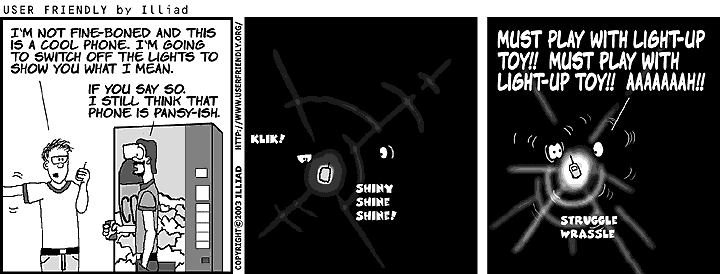
\includegraphics[width=\linewidth]{bilder/comics/uf005633.png}
\end{center}
\newpage
	\begin{multicols}{2}

%%% Local Variables: 
%%% mode: latex
%%% TeX-master: "../../1-te"
%%% End: 

		%\newpage
		%\subsection{Tagebücher}
\subsubsection{Tagebuch eines 1. Semesters\ldots}

\begin{description}
\item[05:30] Der Quarz-Uhr-Timer mit Digitalanzeige gibt ein zaghaftes "`Piep-Piep"'
von sich. Bevor sich dieses zu energischem Gezwitscher entwickelt, sofort
ausgemacht, aus dem Bett gehüpft. Fünf Kilometer Jogging an der Oker,
mit einem Besoffenen zusammengestoßen, anschließend eiskalt geduscht.
\item[06:00] Beim Frühstück Heise-Online studiert und dabei neueste Patches geladen.
Danach kritischer Blick in den Spiegel, Outfit genehmigt.
\item[07:00] Zur Uni gehetzt. PK 2.2 erreicht. Pech gehabt: erste Reihe schon besetzt.
Niederschmetternd. Beschlossen, morgen doch noch eher aufzustehen.
\item[07:30] Vorlesung, Algorithmen und Datenstrukturen bei Fekete. Keine Disziplin!
Einige Kommilitonen lesen
Sportteil der BZ oder gehen ins "`Viertel Nach"' frühstücken. Alles
mitgeschrieben. Füller leer, aber über die Witzchen des Dozenten mitgelacht.
\item[08:00] Vorlesung, Lineare Algebra, Marten. Verdammt! Extra neongrünen Pulli
angezogen und trotz eifrigem Fingerschnippens nicht drangekommen.
\item[10:45] Nächste Vorlesung. Nachbar verläßt mit Bemerkung "`Sinnlose
Veranstaltung"' den Raum. Habe mich für ihn beim Prof. entschuldigt.
\item[12:00] Mensa Essen II. Nur unter größten Schwierigkeiten
weitergearbeitet, da in der Mensa zu laut.
\item[12:45] In Fachschaft gewesen. Mathe Skript immer noch nicht fertig. Wollte
mich beim Vorgesetzten beschweren. Keinen Termin bekommen. Daran geht die
Welt zugrunde.
\item[13:00] Fünf Leute aus meiner Stuko-Gruppe getroffen. Gleich für drei AG's zur
Klausurvorbereitung verabredet.
\item[13:30] Dreiviertelstunde im Copyshop gewesen und die Klausuren der letzten 10
Jahre mit Lösungen kopiert. Dann Kleine übung: Ältere Semester haben keine
Ahnung.
\item[15:30] In der Bibliothek mit den anderen gewesen. Durfte aber statt der
dringend benötigen 18 Bücher nur vier mitnehmen.
\item[16:00] Große übung. War gut vorbereitet. Hinterher den Assi über seine
Irrtümer aufgeklärt.
\item[18:30] Anhand einschlägiger Quellen die Promotionsbedingungen eingesehen und
erste Kontakte geknüpft.
\item[19:45] Abendessen. Verabredung im "`Dialog"' abgesagt. Dafür Vorlesungen
der letzten paar Tage nachgearbeitet.
\item[23:00] Videoaufzeichnung von "`Relationale Datenbanken 1"' angesehen und im Bett noch den "`Cormen"'
gelesen. Festgestellt, 18-Stunden-Tag zu kurz. Werde demnächst die Nacht
hinzunehmen.
\end{description}
\begin{center}
  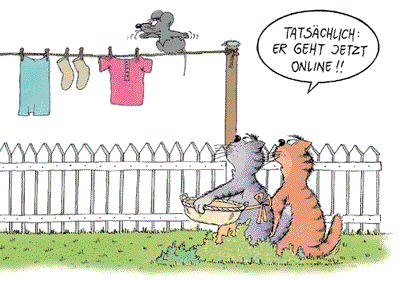
\includegraphics[width=\linewidth]{bilder/comics/stein1.png}
\end{center}
\newpage
\subsubsection{Tagebuch eines 11. Semesters\ldots}

\begin{description}
\item[10.30] Aufgewacht! Ach, Kopfschmerzen, übelkeit, zu deutsch: KATER!
\item[10.45] Der linke große Zeh wird Freiwilliger bei der Zimmertemperaturprüfung.
(Arrgh!) Zeh zurück. Rechts Wand, links kalt; Mist, bin gefangen.
\item[11.00] Kampf mit dem inneren Schweinehund: Aufstehen oder nicht - das ist
hier die Frage.
\item[11.30] Schweinehund schwer angeschlagen, wende Verzögerungstaktik an und
schalte Fernseher ein (inzwischen auch schon verkabelt).
\item[12.05] Mittagsmagazin beginnt. Originalton Moderator: "`Guten Tag liebe
Zuschauer Guten MORGEN liebe Studenten."' Auf die Provokation hereingefallen
und aufgestanden.
\item[13.30] In der Cafeteria der Mensa Katharienstraße beim Skat mein Mittagessen
verspielt.
\item[14.30] Im Hermanns hereingeschaut. Geld gepumpt und 'ne Kleinigkeit
gegessen: Bier schmeckt wieder! Kurze Diskussion mit ein paar Leuten über
die letzte Entwicklung auf dem Computerspielemarkt.
\item[15.45] Kurz in der Bibliothek gewesen. Nix wie raus, total von Erstsemestern
überfüllt.
\item[16.00] Fünf Minuten im IZ gewesen. Nichts los! Keine Zeitung, keine
Flugblätter\ldots
\item[17.00] Stammkneipe hat immer noch nicht geöffnet.
\item[18.15] Resigniert im fgraum ne Flasche Mate geholt und die neuste bbt folge gesehen.
\item[19.10] Komme zu spät zum Date mit dem blonden Erstsemester im Eusebia.
Immer dieser Streß!
\item[01.00] Die Kneipen schließen auch schon immer früher\ldots Umzug ins Jolly Joker.
\item[04.20] Tagespensum erfüllt. Das Bett lockt.
\item[05.35] Am Okerufer von Erstsemester über'n Haufen gerannt worden. Hat mich
gemein beschimpft.
\item[06.45] Bude mühevoll erreicht. Insgesamt \EUR{27,50} ausgegeben. Mehr hatte der
Kleine nicht dabei.
\item[07.05] Schlucke schnell noch ein paar Alkas und schalte kurz das Radio ein.
Stimme des Sprechers: "`Guten Morgen liebe Zuhörer, gute NACHT liebe
Studenten."'
\end{description}
 % inhaltlich fehlerhaft überarbeiten oder ganz raus...
	\newpage
	\section{Gruppen und Unipolitik}
		\label{politik}
		\subsection{Fachgruppe}
\label{fachgruppe}
\url{http://fginfo.cs.tu-bs.de}

Die Fachgruppe seid ihr! Im Grunde besteht die Fachgruppe aus sämtlichen Studierenden der Fachrichtung Informatik. Diese wählen einen Fachgruppenrat der sich dann für die Interessen aller einsetzt. 
Im Fachgruppenraum IZ150 stehen dir jederzeit zuverlässige Mitstudierende zur Verfügung denen du Fragen bezüglich deines Studiums und allem drumherum stellen kannst. Einige davon sind auch Mitglieder des Fachgruppenrats und sind dafür verantwortlich, die Meinungen aller Informatikstudierenden gegenüber der Fakultät und in verschiedenen Kommissionen zu vertreten. Eine richtige Trennung zwischen Fachgruppenrat und Fachgruppe besteht also nicht. Also komm vorbei, bringt dich ein und engagier dich für unsere Studienrichtung. Oder hol dir einfach ein paar koffeinreiche Erfrischungen. 

		%\begin{multicols}{2}
	\subsection*{Studentische Selbstverwaltung für Dummies}
		Seit die '68er durch die deutschen Universitäten gefegt sind, ist Demokratie eingekehrt. Doch was bedeutet das konkret für euch?

	\subsubsection*{Studierendenparlament}
		Eines der wichtigsten Elemente der studentischen Mitbestimmung ist das Studierendenparlament (Uni-Slang: StuPa). Es wird jedes Semester gewählt und entscheidet unter anderem über den studentischen Haushalt, den ihr als Teil des Semesterbeitrags zahlt. Außerdem werden hier Ausschüsse gewählt (Als wichtigster der \emph{Allgemeine Studierenden Ausschuss}, kurz AStA).

	\subsubsection*{AStA}
		Der Allgemeine Studierenden Ausschuss ist die \emph{Exekutive} der Studenten: Er vertritt euch nach Außen, also zum Beispiel bei Verhandlungen um das Semesterticket, versorgt euch mit Informationen zu politischen Themen (öfter im Semester erscheint der so genannte \emph{AStA-Issue}) und ist einer der ersten Ansprechpartner für eure Anliegen.
%REDUNDANT JST
%	\subsubsection*{Fachgruppenrat}
%		Der Fachgruppenrat i
%		Auch der Fachgruppenrat wird von euch gewählt. Allerdings wählt hier jede Fachrichtung ihre eigene, ihr also Fachgruppe Informatik. Da die Fachgruppe euch auch diese Zeitung präsentiert, hat sie sich erlaubt, sich in einem eigenen Abschnitt ab Seite \pageref{fachgruppe} etwas ausführlicher darzustellen.

	\subsubsection*{Gremien}
		In der Uni gibt es unzählige Gremien, hier seien die wichtigsten genannt. Jedes Gremium hat eine bestimmte Besetzung, also eine definierte Anzahl von jeweils Studenten, Mitarbeitern und Professoren.

		Am relevantesten für euch ist die Studienkommission (\emph{StuKo}): Hier werden Details des Studiengangs besprochen, Probleme der Studenten geklärt und die Vergabe der Studiengebühren entschieden. In diesem Gremium herrscht ein Stimmengleichgewicht zwischen Studenten und Professoren. Das bedeutet, dass wir hier wirklich die Möglichkeit haben, aktiv in die Unipolitik einzugreifen.

		In der \emph{Informatik-Kommission} und im
		\emph{Fakultätsrat} (der außerdem noch Mitglieder aus
		den Sozial- und Wirtschaftswissenschaften, sowie der Mathematik hat) sieht es da schon schlechter aus, die Studenten stellen in beiden nur eine Minderheit der Stimmen.

		Die \emph{Berufungskommission} hat nur selten zu tun: Wann immer eine Professur besetzt werden muss, tagt sie um Kandidaten für das Amt zu finden.

		Wann immer ihr Anträge im Prüfungsamt stellt, landen diese im \emph{Prüfungsausschuss}, der entscheidet, ob diese rechtmäßig sind. In diesem sind drei Professoren, ein Student und ein Mitarbeiter vertreten.

	\subsection*{Uniweite Vollversammlung (VV)}
		Mindestens einmal im Semester findet eine
		Vollversammlung aller Studenten statt, d.h. theoretisch
		stürmen 13500 Studenten ins Audimax. Obwohl jeder kommen
		soll, reicht schon ein winziger Bruchteil dessen, damit
		die VV beschlussfähig ist. So können hier wichtige
		Themen abgestimmt werden, die alle Studenten betreffen,
		zum Beispiel wurde die Einführung des Semestertickets
		hier beschlossen. Leider kommt meist nichtmal dieser
		Bruchteil zustande, so dass die VV dann nur Empfehlungen
		an das StuPA aussprechen kann. Wenn ihr informiert darüber 
		bleiben wollt, was neben eurem Studiengang so an der Uni vor sich geht, solltet ihr diese Versammlungen nicht verpassen.

		\subsubsection*{Vollversammlung der Informatik}
			Was vor vielen Jahren noch regelmäßig war, ist
			zwischenzeitlich etwas eingeschlafen. Seit dem
			Sommersemester 2010 gibt es aber wieder VV's der
			Informatikstudenten, auf denen die Fachgruppe
			wichtige Informationen verkündet und einen
			breiteren Dialog sucht, als es über die
			Fachgruppentreffen oder die Mailkommunikation
			möglich ist. Hier ist die möglichkeit für jeden,
			sich mit minimalem Aufwand in die Gestaltung des
			Studienganges einzubringen. Auch hier gilt: Wenn
			20\% der Studenten anwesend sind  ist die VV offiziell beschlussfähig.
	
%\end{multicols}
%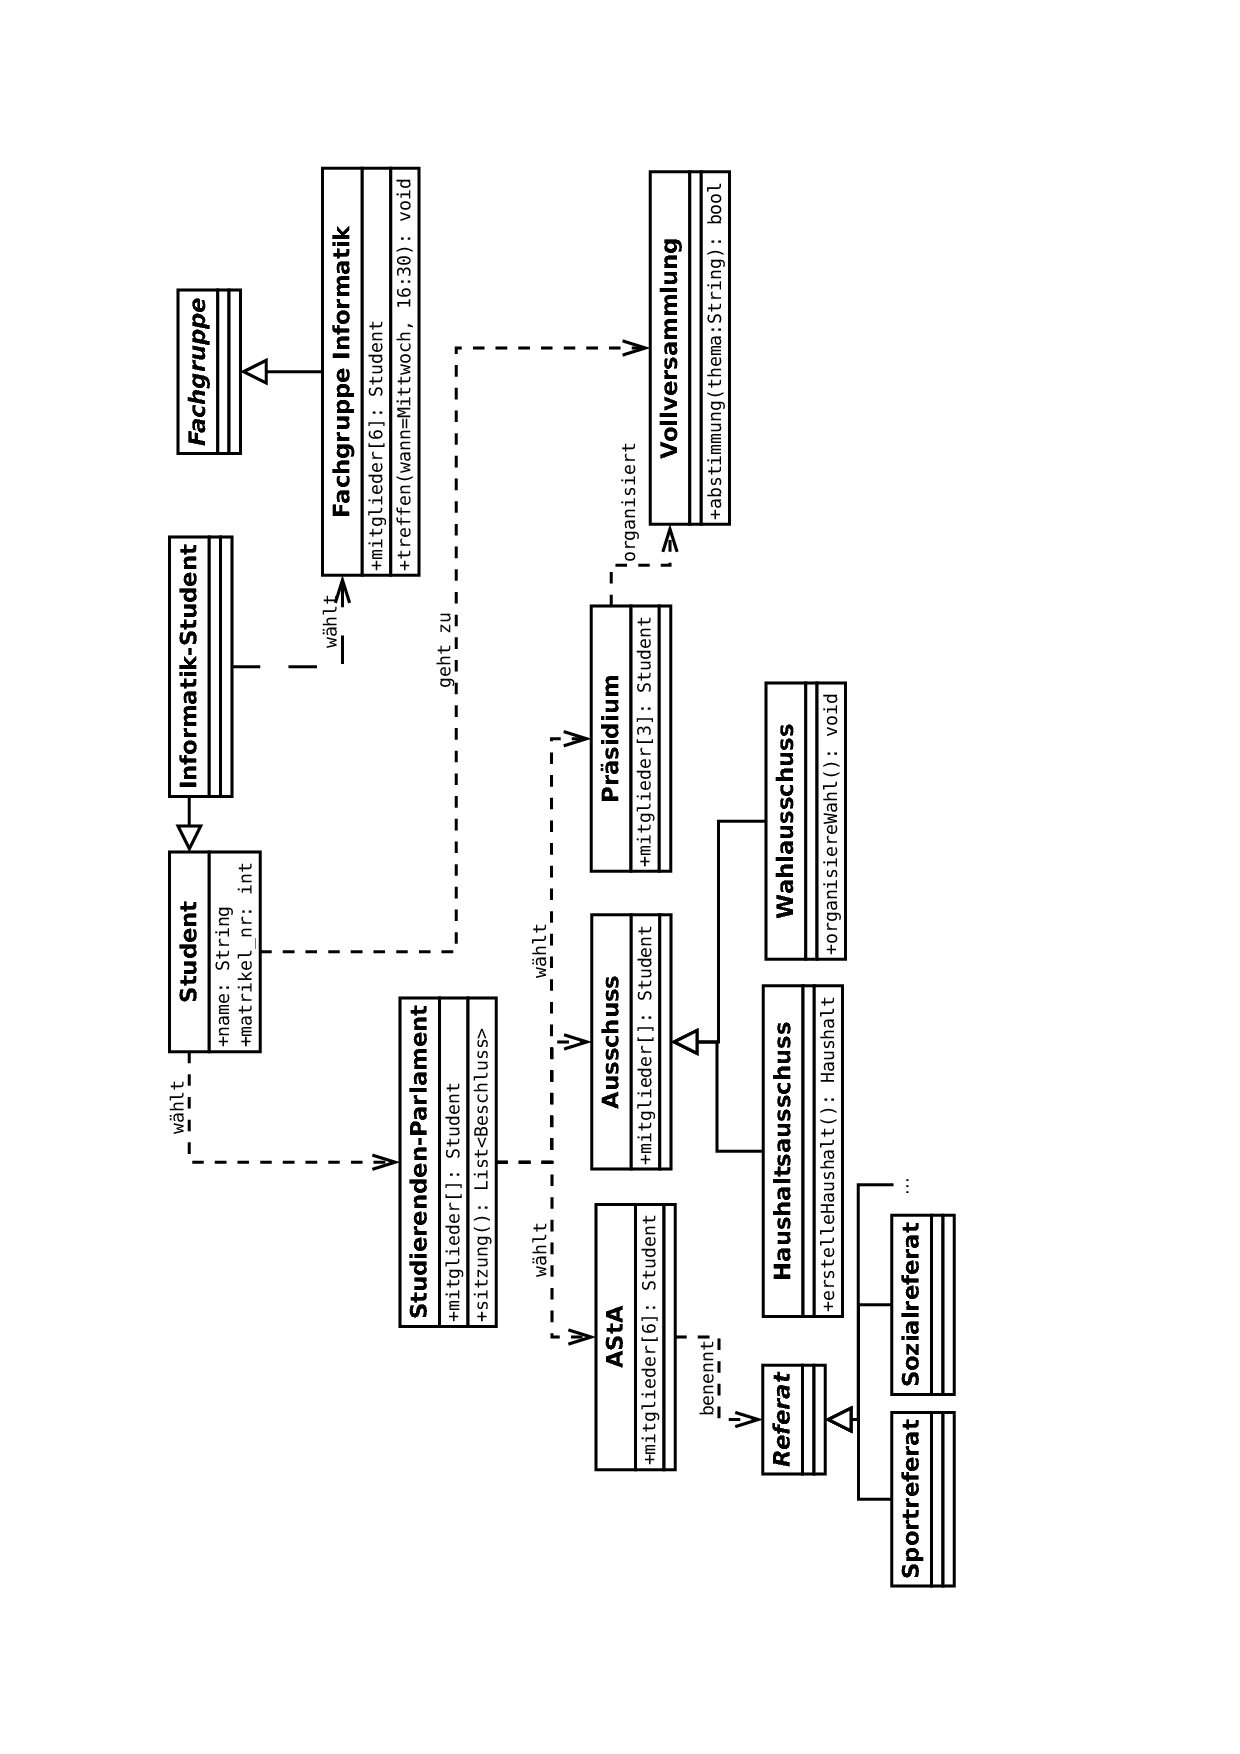
\includegraphics[width=\textwidth]{bilder/gremienkunde2}

		%\begin{multicols}{2}
\subsection{Ich bin unpolitisch!}
	Immer wieder hört man diese Aussage in Vorlesungen, in der Mensa und im Gespräch mit Studierenden beim Fachgruppenrat. Für die meisten Studierenden bedeutet diese Aussage, dass man \emph{kein Interesse an Politik} hat oder zumindest keine Meinung zu aktuellen Vorgängen.

\subsubsection*{Gemäßigtes Braunschweig}

Das Braunschweiger Umfeld macht es einem relativ leicht, sich politisch passiv 
zu verhalten. Hier herrscht nur ein recht kleines Spannungsfeld zwischen den 
traditionell eher rechten studentischen Verbindungen und den traditionell eher 
linken Fachschafts- und Fachgruppenräten sowie dem AStA. Diese 
gegenüberstehenden Parteien werdet ihr in den allermeisten deutschen 
Universitätsstädten wiederfinden. Während es aber anderenorts so richtig 
kracht (Burschenschaftshäuser werden mit Farbbeuteln beworfen und mit Parolen 
beschmiert, jeder öffentliche Auftritt von Burschenschaften führt zu 
Demonstrationen), ist Braunschweig ein gemütliches Pflaster. AStA und die 
Fachschaften finden nur wenige Unterstützer und auch die Burschenschaften 
dominieren in Braunschweig nicht unbedingt das Stadtbild.

\subsubsection*{\emph{Schnell durchziehen!}}

Einen erheblichen Beitrag zur \emph{Ist-mir-doch-egal}-Haltung leistet meiner 
Ansicht nach die heute übliche, ständig über Medien, Politiker oder auch die 
eigenen Eltern verbreitete Doktrin, dass man sein Studium \emph{schnell 
durchziehen}, zielstrebig, leistungs- und ich-orientiert seinen Abschluss 
ansteuern soll. Solche Leute will die Wirtschaft, dafür gibt es Preise und 
Stipendien. Langzeitstudenten werden belächelt und als Sozialfall angesehen. 
Unbequeme Themen wie ethische und religiöse Fragen oder Umweltproblematik 
bleiben bei dieser Sichtweise als erstes auf der Strecke (z.B. gibt es in der 
Informatik in Braunschweig --~anders als zum Beispiel an der Uni Hamburg~-- 
keine Pflichtveranstaltung, die sich mit den gesellschaftlichen Einflüssen der 
Informatik auseinander setzt). Man hat das Gefühl, dass unmündige, 
manipulierbare Arbeitnehmer heranzuzüchtet werden sollen - den früher 
propagierten \emph{breiten Horizont} einer Hochschulausbildung konnte ich an 
unserer TU bisher nicht entdecken.

\subsubsection*{Verbindungen zur Politik}

Nun zurück zum \textbf{weit verbreiteten Gerücht, das eigene Studium habe 
doch nichts mit Politik zu tun}: Die Uni als Institution lässt sich nicht von 
der Politik lösen! Wir sind alle direkt betroffen von der Landespolitik (vor 
allem natürlich Bildungspolitik) und Lokalpolitik (z.B. Radwege, 
Attraktivität der Stadt). Außerdem gibt es auch eine Uni-interne Politik, wie 
euch die \emph{Kleine Gremienkunde} in diesem Heft schon ausführlich dargelegt 
hat. Wer sich z.B. in einem Institut umhört, wird dort nirgends 
Gleichgültigkeit gegenüber der Bildungspolitik zu spüren bekommen. Ob 
Professorenstellen neu besetzt werden, ob genügend HiWis für kleine übungen 
bezahlt werden, ob neue Geräte angeschafft werden, ob gar ganze Studiengänge 
geschlossen werden, ob Studierende bei der Gestaltung ihrer Studiengänge 
mitwirken dürfen, ob öffnungszeiten für bestimmte Dienste verlängert werden 
- all dies hängt von der so viel geschimpften \emph{Politik} der einen oder 
anderen Form ab. \textbf{Politik betrifft euch} und euer Studium. Direkt und 
ohne Wenn und Aber.

Nun will ich natürlich von niemandem verlangen, dass er einer Partei beitritt, 
Straßenaktionen startet oder Bücher schreibt. Aber zumindest ein kleines 
Interesse an eurem direkten Umfeld sollte doch selbstverständlich sein, oder? 
Es hat ja einen Grund, dass euer momentanes Studium so ist, wie es ist. Es gibt 
Studierende, die sich engagieren, die selbst etwas beitragen wollen, z.B. eine 
neue BPO (Bachelorprüfungsordnung) mit erarbeiten, für mehr Computer oder 
längere öffnungszeiten streiten etc., um unseren Studiengang und unser 
Hochschulleben attraktiver zu gestalten.

Übrigens war die Hochschulpolitik bis zum Sommersemester 2011 überwiegend 
unabhängig von parteipolitischen Interessen. Nun sind aber erstmals auch 
Wahllisten angetreten, die etablierten Parteien aus der Landes- und Bundespolitik
nahestehen und dies durch ihren Namen eindeutig aufzeigen. Ob und wie sich dies auf die 
Hochschulpolitik auswirkt, wird sich in den kommenden Semestern zeigen.

\subsubsection*{Informieren und Engagieren}

Wie kann man nun einen Einblick in das, was die Studierenden bewegen und was 
die Studierenden bewegt, gewinnen? Als erstes wären dort die hauptamtlichen 
Mitarbeiter des \textbf{AStA} zu nennen. Hinter der umständlichen Abkürzung 
verbergen sich eine Handvoll Studierende, die entgegen weitläufiger Meinung 
weder Steineschmeißer noch Nazis sondern Studierende wie ihr sind. Dann gibt 
es jeden Monat die \textbf{hochschulöffentliche Sitzung des 
Studierendenparlaments}. Dort tauscht man fächerübergreifend Neuigkeiten aus 
und stimmt über entscheidende Dinge ab, z.B. über die Verwendung der 
studentischen Gelder, den studentischen Haushalt. Mindestens einmal im Semester 
gibt es die sogenannte VV, das ist die \textbf{studentische Vollversammlung} - 
wenn sie beschlussfähig ist, dann ist die Vollversammlung das höchste Gremium 
der Studierenden.
Schließlich finden einmal im Semester die \textbf{studentischen Wahlen} statt 
- da könnt ihr direkt oder indirekt (siehe Gremienkunde) bestimmen, welche 
Studierenden euch in den jeweiligen ämtern vertreten sollen. Aus 
unerfindlichen Gründen ist die Wahlbeteiligung bei den studentischen Wahlen 
stets niedrig. Nehmt das als Aufmunterung -- bei geringer Beteiligung zählt 
eure Stimme um so mehr!
 % redaktionall fragwürdig
		%\subsection[Studiengebühren]{Studiengebühren --\\ eine abschließende
Betrachtung}
\emph{von Henning Günther}

Wir schreiben das Wintersemester 2009/10.
Der Widerstand gegen Studiengebühren liegt in Trümmern.
Nach den vernichtenden Niederlagen im voll\-stän\-di\-gen Boykott der
Studiengebühren im Sommersemster 2007, an dem nur 504 der über 14.000 Studenten teilnahmen und dem darauf folgenden, kaum noch spürbaren ,,5 Euro''-Boykott im Wintersemester 2007/08 sind die Studenten kaum noch zu Widerstand bereit. Im Sommersemster 2008 war das Werk vollbracht, jeder anfängliche Widerstand in alle Winde zerstreut, die anfänglich so breit erscheinende Front der Studiengebührengegner zerschlagen.

Was war geschehen?
Wie konnte sich die vormals so rebellische Studentenschaft, die früher keine Möglichkeit ausließ, gegen das Unrecht zu protestieren, innerhalb von nur einem Jahr in einen in gedemütigter Haltung die Gebühren entrichtenden Haufen Elend verwandeln?

Es hat den Anschein, dass die diabolisch geniale Saat der
Studiengebühren-Fürsprecher, die Daumenschrauben der ,,Campus-Maut'' nicht
sofort und im vollen Umfang anzuziehen, auf ganzer Linie aufgegangen sei. Denn es traf zunächst die, die sich am wenigsten wehren konnten: An Erstsemestern die, da noch nicht eingeschrieben, keinen Boykott wagen
konnten wurde zuerst erprobt, ob 500 Euro ein Preis waren, für den die Studenten zu kämpfen bereit wären. Sie waren es nicht.
Zwar waren viele ,,im Prinzip'' dagegen, taten diese Meinung aber nur mäßig
auf den wenigen Demonstrationen kund.

Die meisten der Studenten scheinen sich inzwischen mit dem Fakt, mit jährlich
1000 Euro weniger auskommen zu müssen, abgefunden zu haben. Kaum jemand gibt sich noch dem Wunschtraum hin, größere Teile der Studenten für irgendeine Form des organisierten Protest zu begeistern.
Es scheint fast als könnten die Studiengebührenschergen bald wieder Morgenluft wittern und in der Lage sein, dank mangelnden Widerstand, ihre kühnsten Träume zu verwirklichen: 1000 Euro Studiengebühren pro Semester und mehr.

Was wird die Zukunft bringen?
Werden die Besiegten weiterhin wie die Gespenster einer längst vergangenen Zeit durch die Unigänge huschen, von einer Vorlesung zur nächsten hetzen, um sich durch ein schnelleres Studium vielleicht ein paar Euro Studiengebühren zu sparen und gelernt haben, stets mit der Angst vor einer Erhöhung der Gebühren zu leben?
Es bleibt zu hoffen dass den Advokaten des Bezahlstudiums dieser Triumph nicht gewährt wird.
%
\end{multicols}
\begin{center}
  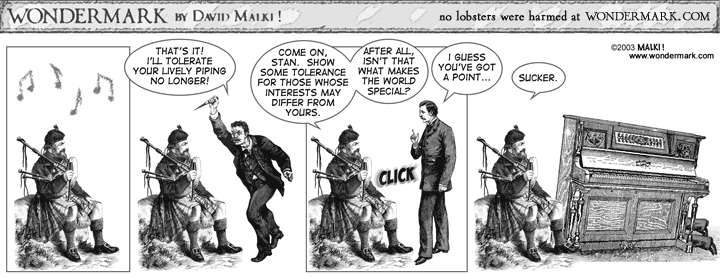
\includegraphics[width=\linewidth]{bilder/comics/wondermark003.png}
\end{center}
%
%
\begin{multicols}{2}
	%da momentan keine einhellige meinung vorherrsct erstmal rauslassen
	\newpage
	\section{Sonstiges}
		\label{sonstiges}
		% !TEX root = ../../1-te.tex

\subsection{Ansprechpartner}

	\paragraph{Fachgruppenrat}
		Im Normalfall treffen wir uns jede Woche zum Fachgruppentreffen im Raum 149/150 des Informatikzentrums. Den  Termin findest du auf unserem Blog \fginfoUrl. Falls du eine Frage hast, kannst du gerne zum regulären Fachgruppentreffen kommen, oder einfach so mal vorbei schauen, ob jemand da ist. Gerade im Semester sind die Chancen gut, einen von uns anzutreffen ;)
		\\
		\\
		Tipp: In der Stunde vor dem Treffen füllt sich der Raum schon langsam, also hast du da gute Chancen, Probleme in kleinerer Runde zu besprechen. Ansonsten erreichst du uns natürlich via Email unter \verHref{6}{mailto:fginfo@tu-bs.de}{fginfo@tu-bs.de}. 

	\paragraph{Fachspezifisches}
		Bei Fragen zu einem speziellen Fach wendest du dich am
		besten an den oder die Professor/in bzw. Dozent/in -
		keine/r von denen beißt! Am besten findest du sie über die Seiten der jeweiligen Institute 
		oder über die Personensuche unter \verUrl{6}{http://www.tu-braunschweig.de/suchoptionen/personen}.

	\paragraph{Studiengangskoordinatorin}
		Yvonne Sehnert \\
		Sie steht bereit, um deine Fragen zu beantworten, und für alles, was sie nicht selbst weiß, weiß sie, an wen sie die Frage weiterleiten muss.\\
		Carl-Friedrich-Gauß-Fakultät\\
		Rebenring 58 A | Raum 124\\
		Sprechzeiten: Nach  Vereinbarung\\
		Telefon: (0531) 391-2843\\
		E-Mail: \verHref{6}{mailto:informatik-studium@tu-bs.de}{informatik-studium@tu-bs.de}

	\paragraph{Prüfungsamt}
		Rebecca Weidner\\
		Carl-Friedrich-Gauß-Fakultät\\
		Rebenring 58 A | Raum 127\\
		Tel.: (0531) 391-2844\\
		Fax: (0531) 391-8220\\
		E-Mail: \verHref{6}{mailto:pa-informatik@tu-braunschweig.de}{pa-informatik@tu-braunschweig.de}\\
		Sprechzeit im Semester:\\
		Di. und Do.: 10:00–12:00 Uhr und 14:00-16:00 Uhr\\
		Sprechzeit in der vorlesungsfreien Zeit:\\
		Di. und Do. 10:00-12:00 Uhr

		\subsection{Lernräume}
	Hier wollen wir euch eine aktuelle Übersicht über Lernräume an der TU Braunschweig geben. Die Liste ist im Moment nicht vollständig. Auf unserem Blog pflegen wir eine Liste, die wir immer dann erweitern, wenn wir einen neuen Lernraum finden.
Wenn du im Laufe deines Studiums einen guten Ort findest, kannst du uns den Raum mitteilen, wir überprüfen das und nehmen ihn dann in die Liste auf.. Alle Gebäude stehen, wenn nicht anders in Anlage 1 der Hausordnung der TU Braunschweig erwähnt, von 7:30 bis 19:30 Uhr offen.
	\subsubsection*{Informatikzentrum}
		\begin{tabular}{|p{4cm}|p{5cm}|p{8cm}|}
			\hline Raum & Öffnungszeiten & Ausstattung \\ 
			\hline Plaza des Informatikzentrums & normal &  Tische und Stühle, Steckdosen unter Bodenabdeckungen zu finden \\
			\hline Fachgruppenraum der Informatik IZ 150 &
			nach Absprache mit Mitgliedern des
			Fachgruppenrates (wir ;) ) & Kaffemaschine,
			Sofas, Tische, WLAN, Steckdosen in Massen sowie Ethernetkabel\\ 
			\hline Fachgruppenraum der Wirtschaftsinformatik
			IZ 159 & nach Absprache mit Mitgliedern des
			Fachgruppenrates Wirtschaftsinformatik & Sofas, Tische, WLAN und Steckdosen \\ 
			\hline CIP Pool IZ G40 & normal & Rechner-Pool mit Linux-PCs, Tafel\\ 
			\hline Gruppenarbeitsraum IZ 033 & 
			
			Solange nicht anders belegt. Den Schlüssel
			erhält man gegen Pfand im Seketariat der Robotik bei Frau Engel,
			Raum G13.
			 &
			Tische, Stühle, WLAN
			\\
			\hline
		\end{tabular}
	\subsubsection*{Andere Lernräume}
		\begin{tabular}{|p{4cm}|p{5cm}|p{3.6cm}|p{4cm}|}
 			\hline Raum & Öffnungszeiten & Ausstattung & Anmerkung  \\  
			\hline Grotrian  Zimmerstraße 24 & Normal  &
			Alte Tische und Stühle, WLAN, vereinzelt Tafeln & Wenn Mitglieder der verschiedenen Fachgruppen anwesend sind hat das Grotrian meist länger offen. Da dies oft der Fall ist kann man hier meist lange lernen. \\ 
			\hline Bibliothek & Mo - Fr: 07:00 - 24:00 Sa:
			10:00 - 20:00& Niedrige Tische und Stühle,
			Ruhezone, WLAN, Rechnerarbeits\-plätze, Kopierer &  nicht zum  Lernen in der Gruppe  geeignet \\ 
			\hline Mensa / Cafeteria & Mo -Do: 08 - 20:00 Uhr Fr: 08:00 - 15:00 & Tische, Stühle, kein (!) WLAN, einzelner Rechner mit Netzzugang, Verpflegung incl. Selbstbedienungs-Kaffeeautomat& Probleme: Nicht durchgehend geöffnet, die Plätze sind primär zu Essen gedacht, von Lernsessions zu den Stoßzeiten sollte man also im eigenen und fremden Interesse absehen. \\ 
			\hline Bei dir zuhause & immer & Deine Sache & Achtung: Ablenkung ;) \\ 
			\hline Das eine oder andere Cafe / Kneipe & kommt drauf an & wechselhaft &Siehe die beiden vorherigen \\
			\hline
		\end{tabular}

		\begin{multicols}{2}
\subsection{Semesterticket}
	Euer Studentenausweis berechtigt euch zur Fahrt auf vielen Zugstrecken in Niedersachsen. Unten seht ihr den Gültigkeitsbereich des Semestertickets im Großraum Hannover. Nach Norden und und Westen deckt das Semesterticket weitere Strecken ab. Einen grober Überblick gibt die nebenstehende Karte. 

	Es dürfen nur Regionalexpress (RE) und Regionalbahn (RB) der Deutschen Bahn AG, sowie teilweise der Metronom in der zweiten Klasse benutzt werden. Also NICHT Strecken der Nordwestbahn (NWB). Einen genauen Überblick findet ihr in Form einer Streckenliste auf der Seite \pageref{streckenliste1}.

	Mehr Details könnt ihr den Seiten des AStA unter \url{http://www.asta.tu-bs.de/semesterticket.php} bzw. \url{http://tinyurl.com/3gn8fhg} entnehmen.
\end{multicols}
\newpage
%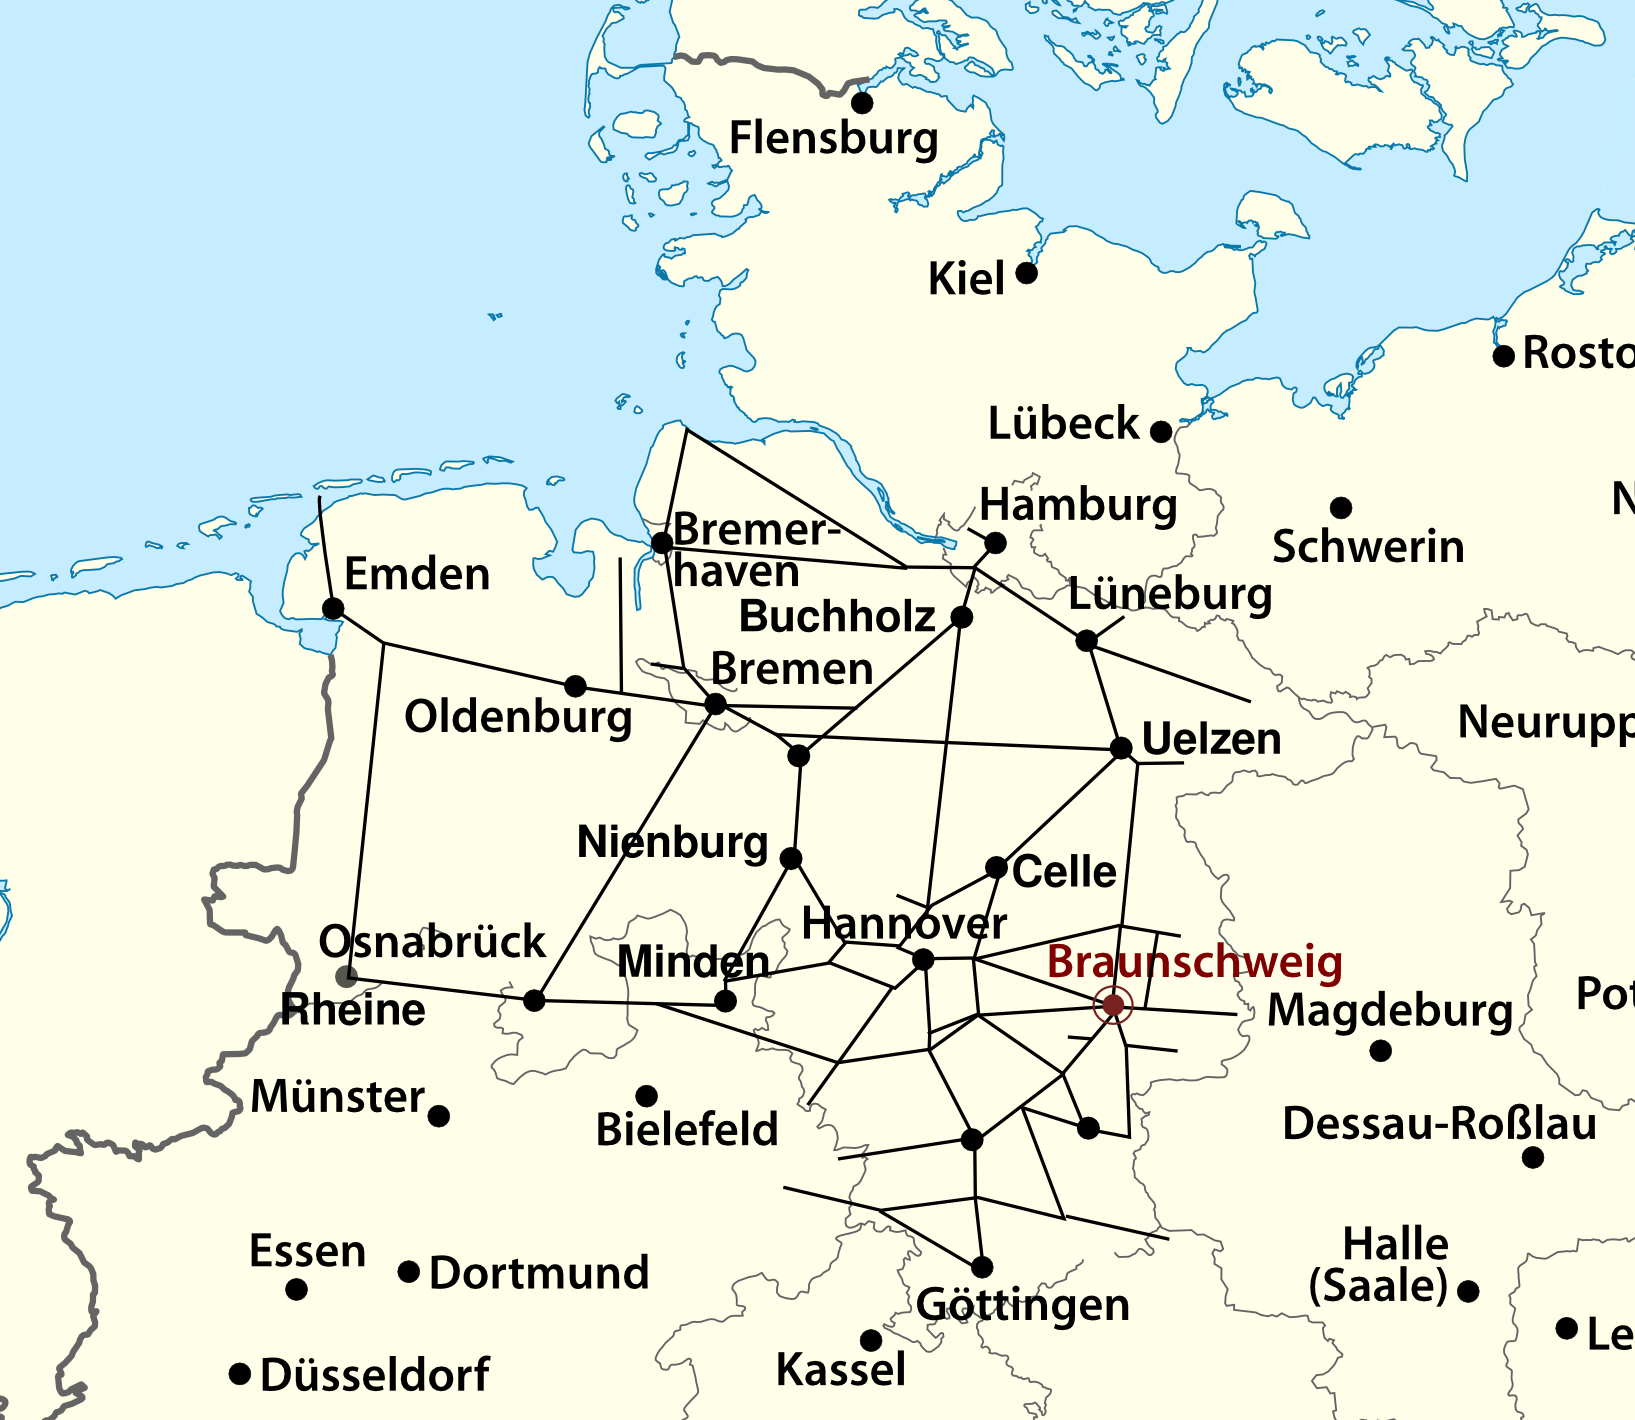
\includegraphics[width=\columnwidth]{bilder/ticket_deutschland.png}
\newpage
%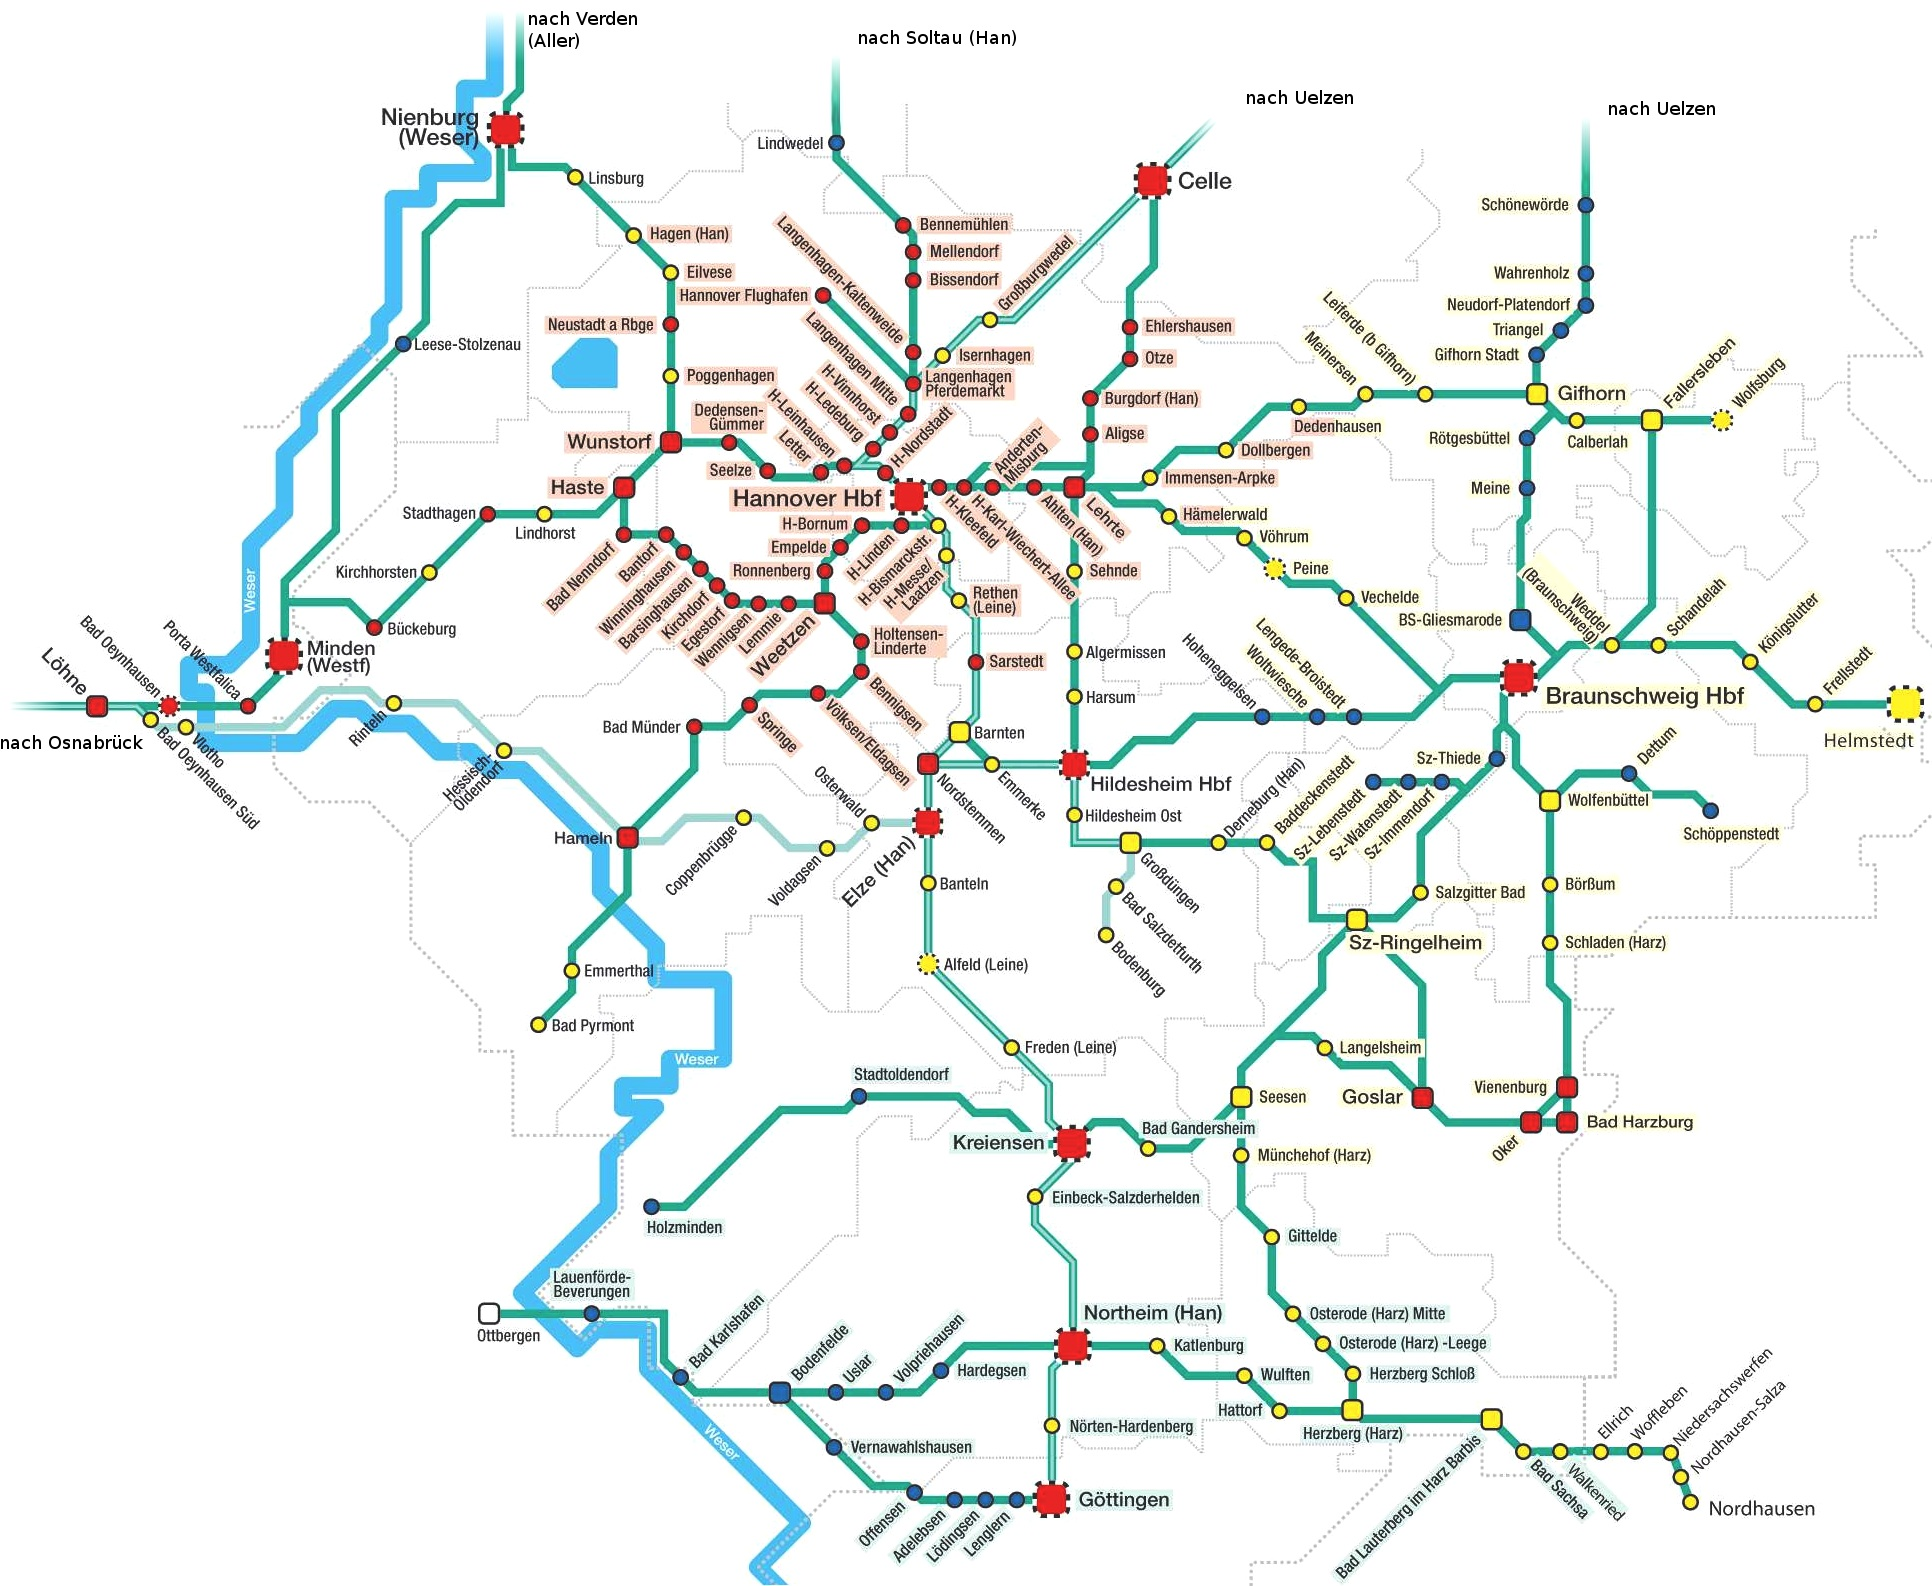
\includegraphics[width=\textwidth]{bilder/ticket_bis_11_Dezember.jpg}
\newpage
\newpage
\begin{multicols}{2}
\subsubsection*{Streckenübersicht Wintersemester 2010/2011 und Sommersemester 2011 gültig ab 1.10.2010}
\label{streckenliste1}
\begin{tabular}{|l|l|l|p{2cm}|}
\hline
\multicolumn{3}{|l|}{\textbf{Strecke/ Streckenabschnitt}}& \textbf{KbN}\\
\textbf{\textit{von}} & \textit{über} & \textbf{\textit{bis}} & \\ \cline{ 1- 4}
Lüneburg &  & Dannenberg Ost & 112 \\ \hline
Braunschweig Hbf & Gifhorn & Uelzen & 115 \\ \hline
Bremen Hbf & Soltau & Uelzen & 116 \\ \hline
Hamburg-Harburg &  & Stade & 121 \\ \hline
Buchholz (Nordheide) & Soltau & Bennemühlen & 123 \\ \hline
Minden Westf. & Nienburg & Rotenburg/Bremen Hbf & 124 \\ \hline
Bremen Hbf &  & Cuxhaven & 125 \footnotemark[1] \\ \hline
Bremen Hbf &  & Bremen-Vegesack & 126 \footnotemark[1] \\ \hline
Echem &  & Lüneburg & 145 \\ \hline
Hannover Hbf & Gifhorn & Wolfsburg Hbf & 300 \\ \hline
Braunschweig Hbf &  & Wolfsburg Hbf & 301 \\ \hline
Uelzen &  & Schnega & 305 \\ \hline
Hannover Hbf & Braunschweig Hbf & Helmstedt & 310 \\ \hline
Braunschweig Hbf & Wolfenbüttel & Schöppenstedt & 312 \footnotemark[2] \\ \hline
Braunschweig Hbf &  & Hildesheim Hbf & 313 \\ \hline
Hannover Hbf & Hildesheim Hbf/Goslar & Bad Harzburg & 320 \\ \hline
Braunschweig Hbf &  & Sz-Lebenstedt & 352 \\ \hline
Braunschweig Hbf & Wolfenbüttel/Vienenburg & Goslar & 353 \\ \hline
Holzminden & Kreiensen & Bad Harzburg & 354 \\ \hline
Ottbergen & Bodenfelde & Göttingen & 356.1 \\ \hline
Ottbergen & Bodenfelde & Northeim & 356.2 \\ \hline
Göttingen & Northeim & Walkenried & 357 \footnotemark[1] \\ \hline
Braunschweig Hbf & Seesen & Herzberg (Harz) & 358 \\ \hline
Haste & Hannover Hbf/Haste & Minden (Westf) & 360.1 \\ \hline
Nienburg (Weser) & Hannover Hbf & Haste & 360.2 \\ \hline
Hannover Hbf & Lehrte & Hildesheim Hbf & 360.3 \\ \hline
Bennemühlen & Hann./Sarstedt & Hildesheim Hbf & 360.4 \\ \hline
Bad Pyrmont & Hameln/Weetzen & Hannover-Flughafen & 360.5 \\ \hline
Celle & Lehrte & Hannover Hbf & 360.6.7 \\ \hline
Hannover Hbf &  & Hannover Bismarckstr. & 361 \footnotemark[1] \\ \hline
Hannover Hbf &  & Löhne (Westf.) & 370 \\ \hline
Löhne (Westf.) & Hameln & Hildesheim Hbf & 372 \\ \hline
Hildesheim Hbf &  & Bodenburg & 373 \\ \hline
Salzbergen & Osnabrück Hbf & Minden (Westf.) & 375 \footnotemark[1] \\ \hline
Bremen Hbf &  & Hannover Hbf & 380 \\ \hline
Osnabrück Hbf &  & Bremen Hbf & 385 \footnotemark[1] \\ \hline
Norddeich Mole & Oldenburg (Oldb) & Bremen Hbf & 390 \footnotemark[1] \\ \hline
Norddeich Mole & Meppen & Rheine & 395 \footnotemark[1] \\ \hline
Emden Hbf &  & Emden Außenhafen & 396 \\ \hline
Leer (Ostfr.) &  & Weener & 397 \\ \hline
\end{tabular}

\footnotetext[1]{nur in den Zügen der DB Regio AG, also nicht in Zügen der Nordwestbahn}
\footnotetext[2]{gültig auch in Bus von  Schöppenstedt-Schöningen-Helmstedt}
\end{multicols}

		% !TEX root = ../1-te.tex

\begin{description}
\item[Herausgeber:]
	Fachgruppe Informatik\\
	c/o AStA der TU Braunschweig\\
	Katharinenstraße 1\\
	38106 Braunschweig\\
	Tel.: 0531/391-4569\\
	E-Mail: \verHref{5}{mailto:fginfo@tu-bs.de}{fginfo@tu-bs.de}\\
	Webseite: \fginfoUrl
\tocheck{4}{Mitglieder das FG-Rats nennen}
\item[Cover:] Sophia Scholtka und Rebecca Finster
\item[Comics:] Randall Munroe -- XKCD (\verUrl{5}{http://xkcd.com/})
\end{description}

\end{document}
